%--------------------------------------------------------------------------
% Dokumentenklasse
%--------------------------------------------------------------------------

% disable Warning for remreset Package
% \RequirePackage{silence}
% \WarningFilter{remreset}{The remreset package}

\documentclass[
	pagesize,
	fontsize=12pt,
	paper=a4,
	oneside,
   reqno
]{scrartcl}

%--------------------------------------------------------------------------
% Standardpakete 
%--------------------------------------------------------------------------
\usepackage[ngerman]{babel}               % Deutsch Silbentrennung
\usepackage[T1]{fontenc}                  % Font Type
\usepackage[utf8]{inputenc}               % Font Encoding
\usepackage{lmodern}                      % Latin Modern Font
\usepackage{csquotes}                     % Setzen von Zitaten
\usepackage{xspace}                       % setzten von Leerzeichen nach Abkürzungen
\usepackage{microtype}                    % für glattere Seitenränder
\renewcommand*\familydefault{\sfdefault}  % Serifen lose Schrift
%\renewcommand*\familydefault{\ttdefault} % Schreibmaschinenschrift

%--------------------------------------------------------------------------
% Extra Packages
%--------------------------------------------------------------------------

% Abkürzungspaket
\usepackage{acronym}

% Symbolverzeichnis
\usepackage[symbols,nogroupskip,nonumberlist,sort=use]{glossaries-extra}

% \makenoidxglossaries

\glsxtrnewsymbol[description={Gewichtskraft}]{FG}{\ensuremath{F_{\mathrm{G}}}}
\glsxtrnewsymbol[description={Gewichtskraft in Bewegungsrichtung}]{FG1}{\ensuremath{F^{'}_{\mathrm{G}}}}
\glsxtrnewsymbol[description={Bewegungskraft des Schlittens}]{Fa}{\ensuremath{F_{\mathrm{a}}}}
\glsxtrnewsymbol[description={Pendelkraft}]{FP}{\ensuremath{F_{\mathrm{P}}}}
\glsxtrnewsymbol[description={Pendelkraft in Bewegungsrichtung}]{FP1}{\ensuremath{F^{'}_{\mathrm{P}}}}
\glsxtrnewsymbol[description={Reibkraft}]{Ff}{\ensuremath{F_{\mathrm{f}}}}
\glsxtrnewsymbol[description={Coulombsche Reibung}]{FC}{\ensuremath{F_{\mathrm{C}}}}
\glsxtrnewsymbol[description={Gesamtkraft}]{Fges}{\ensuremath{F_{\mathrm{ges}}}}
\glsxtrnewsymbol[description={Pendelmoment}]{MP}{\ensuremath{M_{\mathrm{P}}}}
\glsxtrnewsymbol[description={Gewichtsmoment}]{MG}{\ensuremath{M_{\mathrm{G}}}}
\glsxtrnewsymbol[description={Reibmoment}]{Mf}{\ensuremath{M_{\mathrm{f}}}}
\glsxtrnewsymbol[description={Gesamtmoment}]{Mges}{\ensuremath{M_{\mathrm{ges}}}}

% Mathe Pakete
\usepackage{amsmath}
\numberwithin{equation}{section}
\DeclareMathOperator{\sgn}{sgn}
\usepackage{thmtools}
\usepackage{amsfonts}
\usepackage{amssymb}
\usepackage{mathtools}
\usepackage{breqn}
\usepackage{empheq}
\usepackage{xfrac}

% Listenumgebungen
\usepackage{listings}
\usepackage{paralist}
\usepackage{enumitem}
\usepackage{adjustbox}

% Demo Text
\usepackage{blindtext}

% Farb-Pakete
\usepackage{xcolor}
\usepackage{fancyvrb}
\usepackage{colortbl}

% Farbedefinitionen
\definecolor{htw}{RGB}{120, 184, 2}
\definecolor{ccW}{RGB}{255,255,255}
\definecolor{ccR}{RGB}{197,14,31}
\definecolor{ccG}{RGB}{113,113,113}
\definecolor{ccL}{RGB}{220,220,220}
\definecolor{ccS}{RGB}{0,0,0}
\definecolor{ccB}{RGB}{68,73,159}
\definecolor{ccD}{RGB}{0,0,80}
\definecolor{grey}{RGB}{200,200,200}
\definecolor{lightGrey}{RGB}{230,230,230}

% Für erweiterte Tabellen
\usepackage{longtable}
\usepackage{tabularx}
\usepackage{float}
\usepackage{multirow}
\usepackage{makecell}
\numberwithin{table}{section}
% \setlength{\tabcolsep}{0.5em}       % for the horizontal padding
% {\renewcommand{\arraystretch}{1.8}  % for the vertical padding
% \usepackage{ragged2e}
% \newcolumntype{R}[1]{>{\RaggedRight}p{#1}}

% Einheitenpaket
\usepackage[exponent-product = \cdot]{siunitx}
\sisetup{locale=DE}
\sisetup{parse-numbers = false}

\makeatletter
\renewcommand\@dotsep{5}
\makeatother

% Pakete für Grafiken
\usepackage{graphicx}
\usepackage{wrapfig}
\usepackage{overpic}
\usepackage{epstopdf}
\usepackage{caption}
\usepackage{subcaption}
\usepackage{rotating}
\usepackage{lscape}
\numberwithin{figure}{section}
\captionsetup[subfigure]{list=true, font=tiny, labelformat=brace, position=top} %setup für subfigure captions

% Diagramm-/Grafikerstellung
\usepackage{pstricks}
\usepackage{tikz}
\usetikzlibrary{patterns,patterns.meta}
\usetikzlibrary{decorations.markings}
\makeatletter
\pgfkeys{/pgf/.cd,
  parallelepiped offset x/.initial=2mm,
  parallelepiped offset y/.initial=2mm
}
\pgfdeclareshape{parallelepiped}
{
  \inheritsavedanchors[from=rectangle] % this is nearly a rectangle
  \inheritanchorborder[from=rectangle]
  \inheritanchor[from=rectangle]{north}
  \inheritanchor[from=rectangle]{north west}
  \inheritanchor[from=rectangle]{north east}
  \inheritanchor[from=rectangle]{center}
  \inheritanchor[from=rectangle]{west}
  \inheritanchor[from=rectangle]{east}
  \inheritanchor[from=rectangle]{mid}
  \inheritanchor[from=rectangle]{mid west}
  \inheritanchor[from=rectangle]{mid east}
  \inheritanchor[from=rectangle]{base}
  \inheritanchor[from=rectangle]{base west}
  \inheritanchor[from=rectangle]{base east}
  \inheritanchor[from=rectangle]{south}
  \inheritanchor[from=rectangle]{south west}
  \inheritanchor[from=rectangle]{south east}
  %\backgroundpath{
  %  % store lower right in xa/ya and upper right in xb/yb
  % \southwest\pgf@xa=\pgf@x\pgf@ya=\pgf@y
  % \northeast\pgf@xb=\pgf@x\pgf@yb=\pgf@y
  % \pgfmathsetlength\pgfutil@tempdima{\pgfkeysvalueof{/pgf/parallelepiped offset x}}
  % \pgfmathsetlength\pgfutil@tempdimb{\pgfkeysvalueof{/pgf/parallelepiped offset y}}
  % \def\ppd@offset{\pgfpoint{\pgfutil@tempdima}{\pgfutil@tempdimb}}
  % \pgfpathmoveto{\pgfqpoint{\pgf@xa}{\pgf@ya}}
  % \pgfpathlineto{\pgfqpoint{\pgf@xb}{\pgf@ya}}
  % \pgfpathlineto{\pgfqpoint{\pgf@xb}{\pgf@yb}}
  % \pgfpathlineto{\pgfqpoint{\pgf@xa}{\pgf@yb}}
  %  \pgfpathclose
  %  \pgfpathmoveto{\pgfqpoint{\pgf@xb}{\pgf@ya}}
  %  \pgfpathlineto{\pgfpointadd{\pgfpoint{\pgf@xb}{\pgf@ya}}{\ppd@offset}}
  %  \pgfpathlineto{\pgfpointadd{\pgfpoint{\pgf@xb}{\pgf@yb}}{\ppd@offset}}
  %  \pgfpathlineto{\pgfpointadd{\pgfpoint{\pgf@xa}{\pgf@yb}}{\ppd@offset}}
  %  \pgfpathlineto{\pgfqpoint{\pgf@xa}{\pgf@yb}}
  %  \pgfpathmoveto{\pgfqpoint{\pgf@xb}{\pgf@yb}}
  %  \pgfpathlineto{\pgfpointadd{\pgfpoint{\pgf@xb}{\pgf@yb}}{\ppd@offset}}
  %}
}
\makeatother
\usetikzlibrary{math}
\usepackage{pgfplots}
%\pgfplotsset{compat=1.5}
\usetikzlibrary{intersections,positioning,arrows,automata,calc,patterns,shapes.multipart,fit,backgrounds,decorations.pathreplacing}
\usetikzlibrary{decorations,shapes.geometric}
\usetikzlibrary{matrix,calc,angles,positioning,quotes}
% \usepackage{tikz-uml}

\usepackage{pgfkeys}
\usepackage{pgfopts}
\usepackage{ifthen}
\usepackage{xstring}
\usepackage{calc}
\usepackage{pst-plot,pst-bar,pst-node} % Balkendiagramme
\usepackage{capt-of}
\usepackage{incgraph} % Fullscreen Images
\usepackage{pdfpages} % Include external pdf pages

\usepackage{latexsym}
\usepackage{censor}
\usepackage{here}
% \StopCensoring        % Auskommentiert wird der Text entschwaerzt 
% \censor{Oszilloskop}  % Befehl zum einschwärzen
\usepackage{trfsigns}   % Transformation Symbol o---o \laplace and \Laplace
\usepackage{circuitikz}

\usepackage{multido}
\usepackage{amsmath}

% Verlinkungen im Text
\usepackage{url}
\usepackage{hyperref}
\PassOptionsToPackage{hyphens}{url}
\hypersetup{hidelinks}
\urlstyle{same}
%\usetikzlibrary{external}
%\tikzexternalize[prefix=figures/]
%--------------------------------------------------------------------------
% Eigene Befehle
%--------------------------------------------------------------------------
\newcommand*\widefbox[1]{\fbox{\hspace{1em}#1\hspace{1em}}} % Box für align-Umgebung

\newcommand{\mycomment}[1]{} % zum Auskommentieren von Tex-Blöcken

%------------sectioning command-------------------
% The sectioning command one level down the hierarchy from \subsubsection is called \paragraph followed by \subparagraph
% to include this in your table of contents

% Tiefe des Inhaltsverzeichnis
\setcounter{tocdepth}{3}
\setcounter{secnumdepth}{4}

% Abkürzungen durch Kommandos setzen
\newcommand{\bspw}{bspw.\xspace}
\newcommand{\bzw}{bzw.\xspace}
\newcommand{\etc}{etc.\xspace}
\newcommand{\zB}{z.\,B.\xspace}
\newcommand{\EV}{e.\,V.\xspace}
\newcommand{\zT}{z.\,T.\xspace}
\newcommand{\iVm}{i.\,V.\,m.\xspace}
\newcommand{\idR}{i.\,d.\,R.\xspace}
\newcommand{\ihv}{i.\,H.\,v.\xspace}
\newcommand{\ua}{u.\,a.\xspace}
\newcommand{\dH}{d.\,h.\xspace}
\newcommand{\vgl}{vgl.\xspace}
\newcommand{\ca}{ca.\xspace}
\newcommand{\dV}{d.\,Verf.}
\newcommand{\RNr}{Rn.\xspace}
\newcommand{\oa}{o.\,{ä}.\xspace}
\newcommand{\vC}{v.\,Chr.\xspace}
\newcommand{\nC}{n.\,Chr.\xspace}
\newcommand{\vA}{v.\,a.\xspace}
\newcommand{\eng}{engl.\xspace}
\newcommand{\tabitem}{~~\llap{\textbullet}~~}

%------------Zitate-------------------------------
\newcommand*{\zitat}[2]{%
   \normalfont\small
   \begin{quote}
   \glqq#1\grqq\par
   #2
   \end{quote}
   \normalsize
}
\newcommand*{\zitatmitueberschrift}[3]{%
   \normalfont\small
   \begin{quote} #3
   \glqq#1\grqq\par
   #2
   \end{quote}
   \normalsize
}
\newcommand*{\zitext}[2]{%
   \glqq#1\grqq\ %
   [#2]%
}

%-----------Seitendesign--------------------------
\usepackage[width=15.5cm, height=23cm, includeheadfoot]{geometry}
\geometry{paper=a4paper}
% \usepackage[left=6cm,right=1cm,top=1.5cm, bottom=1cm, includeheadfoot]{geometry}
% \newgeometry{oneside}
% \setlength{\voffset}{0cm}
\setlength{\headheight}{1.1\baselineskip} % increase headheight
\setlength{\footheight}{28.99998pt}       % increase foodheight
\setlength{\parindent}{0cm}               % Einrücken nach \newline
\setlength{\footskip}{86pt}               % Move Footer down
% \setlength{\topmargin}{0cm}
% \setlength{\marginparsep}{0.5cm}
% \setlength{\marginparwidth}{1.5cm}
% \setlength{\textwidth}{16cm}
% \setlength{\textheight}{23cm}
% \setlength{\oddsidemargin}{1cm}
% \setlength{\evensidemargin}{2cm}

%----------Kopf & Fußzeile------------------------
% \usepackage[headsepline,footsepline]{scrlayer-scrpage}
\usepackage[headsepline]{scrlayer-scrpage}
\pagestyle{scrheadings}
\clearpairofpagestyles%
\ihead{\headmark}
\automark{section}
\chead{}
\ohead{
\includegraphics[scale=0.09]{Bilder/HTWLogoKopfzeile.png} \nocite{HTWklein}}
\cfoot{\pagemark}
\ofoot{M2 Modellbildung/\\ Simulation}

% Aaron Page Style
\newpairofpagestyles[scrheadings]{aaron}{%
    \ifoot{Aaron\\ Zielstorff}
}

% Sebastian Page Style
\newpairofpagestyles[scrheadings]{sebastian}{%
    \ifoot{Sebastian\\ Richter}
}

% Milan Page Style
\newpairofpagestyles[scrheadings]{milan}{%
    \ifoot{Milan\\ Larsen}
}

% Cyrill Page Style
\newpairofpagestyles[scrheadings]{cyrill}{%
    \ifoot{Cyrill\\ Schmiedehausen}
}

%--------------------------------------------------------------------------
% Beginn des Dokuments
%--------------------------------------------------------------------------
\begin{document}

%----------Deckblatt----------------------------- 
\begin{titlepage}
   \pagestyle{empty} % setzt Pagestyle-Befehl

   % HTW Logo
   \begin{flushright}
   
\includegraphics[scale=.07]{Bilder/LogoHTWBerlin.png}  \nocite{HTWgross}
   \end{flushright}

   \vspace{1cm}

   % Titel
   \begin{center}
      \Huge{\textbf{Schwungrad Pendel: Modellbildung/Simulation (M2)}} \\
   \end{center}

   \vspace{3cm}

   % Name
   \begin{flushleft}
      \begin{tabular}{l c l}
         \textbf{Name: }&\hspace{1 cm} &\textbf{Matrikelnummer:} \\
         Milan Larsen           & & 581929 \\
         Sebastian Richter      & & 572906 \\
         Cyrill Schmiedehausen  & & XXXXXX \\
         Aaron Zielstorff       & & 567183 \\
      \end{tabular}
   \end{flushleft}

   \vspace{1cm}

   % Daten
   \begin{tabular}{l l}
      \textbf{Fachbereich:}   & FB1                                                     \\
      \textbf{Studiengang:}   & M.\xspace Elektrotechnik                                \\
      \textbf{Fachsemester:}  & 2.\xspace FS                                            \\
      \textbf{Fach:}          & M2 Modellbildung/Simulation                             \\
      \textbf{Dozent:}        & Prof.\xspace Dr.\xspace -Ing.\xspace Steffen Borchers   \\
      \textbf{Abgabe am:}     & 23.\xspace September 2022                               \\ 
   \end{tabular}
\end{titlepage}
\clearpage

%--------Inhaltsverzeichnis-----------------------
\renewcommand{\contentsname}{Inhaltsverzeichnis}
\tableofcontents
\clearpage

%--------Abbildungsverzeichnis--------------------
\renewcommand{\listfigurename}{Abbildungsverzeichnis}
\renewcommand*{\figurename}{Abb.}
\listoffigures
% \clearpage

%--------Tabellenverzeichnis----------------------
\renewcommand*{\listtablename}{Tabellenverzeichnis}
\renewcommand*{\tablename}{Tab.}
\listoftables
\clearpage

%----------Symbolverzeichnis----------------------
% \printnoidxglossary[type=symbols,style=long,title={Symbolverzeichnis}]
% \clearpage

%---------Kapitel/Text----------------------------

\pagestyle{aaron}
\section{Einführung und Versuchsaufbau} \label{sec:Einfuehrung}

Inhalt dieser Belegarbeit ist die Modellierung eines inversen Pendels, welches über ein Schwungrad regelungstechnisch in der aufrechten Position stabil gehalten werden soll.\\
Diese Arbeit geht dabei im ersten Abschnitt auf den \textbf{Versuchsaufbau} und die \textbf{Modellierung} des Pendels ein. Es schließt sich eine \textbf{Sensitivitäts- und Parameteranalyse} an, über welche der Einfluss bestimmter Modellgrößen auf das Verhalten des Systems untersucht wird. \\
Nachdem das Modell aufgestellt und auf seine Eigenschaften analysiert wurde, folgt die Implementierung als Simulation in Matlab/Simulink. Dafür soll zunächst das \textbf{Aufschwingen des Pendels}. umgesetzt werden. Kann das Pendel bis in einen bestimmten Bereich um die obere Ruhelage bewegt werden, übernimmt ein \textbf{einfacher Zustandsregler}, welcher ebenfalls in dieser Arbeit entworfen wird. \\
Abschließend wird ein \textbf{Beobachter} umgesetzt, über welchen die nicht messbaren Zustände des Systems rekonstruiert werden können, um den Regler am realen Versuch in Betrieb zu nehmen.

Nachfolgend findet sich die Darstellung der Modellparameter/Konstanten zur Modellierung des Schwungrad-Pendels (siehe \autoref{tab:Tabelle1.1}).

\begin{table}[H]
    \centering
    \begin{tabular}{|lll|}
        \hline
        \rowcolor{grey}
        \textbf{Symbol}     & \textbf{Parameter}                                & \textbf{Wert/Einheit}                         \\ \hline
        $\theta$            & Winkel des Pendels                                & $\SI{}{rad}$                                  \\
        $\varphi$           & Winkel des Schwungrades                           & $\SI{}{rad}$                                  \\
        $J_{\mathrm{1}}$    & Trägheitsmoment des Pendels (+ Motorstator)       & $\SI{0.01186}{kg \cdot m^2}$                  \\
        $J_{\mathrm{2}}$    & Trägheitsmoment des Rads (+ Motorrotor)           & $\SI{0.0005711}{kg \cdot m^2}$                \\
        $c_{\mathrm{1}}$    & Reibungsfaktor des Pendels                        & $\SI{0.04}{\frac{N \cdot m \cdot s}{rad}}$    \\
        $c_{\mathrm{2}}$    & Reibungsfaktor des Rads                           & $\SI{0.0001}{\frac{N \cdot m \cdot s}{rad}}$  \\
        $m_{\mathrm{1}}$    & Masse des Pendels und Stators                     & $\SI{0.826}{kg}$                              \\
        $m_{\mathrm{2}}$    & Masse des Rads und Rotors                         & $\SI{0.583}{kg}$                              \\
        $l_{\mathrm{1}}$    & Länge vom Ursprung bis Schwerpunkt des Pendels    & $\SI{0.1053}{m}$                              \\
        $l_{\mathrm{2}}$    & Länge vom Ursprung bis Schwerpunkt des Rads       & $\SI{0.14}{m}$                                \\
        $K_{\mathrm{b}}$    & Back-End-Konstante                                & $\SI{0.0987}{\frac{V}{\frac{rad}{s}}}$        \\
        $K_{\mathrm{t}}$    & Motor-Drehmoment-Konstante                        & $\SI{0.0987}{\frac{N \cdot m}{A}}$            \\
        $R_{\mathrm{a}}$    & Widerstand der Ankerwicklung                      & $\SI{1.5562}{\Omega}$                         \\ \hline
    \end{tabular}
    \caption{Modellparameter des Schwungrad-Pendels}
    \label{tab:Tabelle1.1}
\end{table}

Ziel der Arbeit soll es sein, anhand von Beispielparametern eine effektive Regelung umzusetzen, welche später bei der Übernahme auf einen realen Versuchsaufbau einfach adaptiert werden kann. Dazu ist es wichtig ein gutes Modell umzusetzen und den Einfluss der verschiedenen Modell- und Regelparameter auf das Verhalten des Systems zu kennen.\\

\autoref{fig:Bild1.1} zeigt den modellhaften Versuchsaufbau. Das System besteht aus einem Pendel und einem Schwungrad. Das Pendel kann frei rotieren um die 0z-Achse, die senkrecht zur 0xy-Ebene steht. Das Schwungrad wird durch einen Gleichstrommotor angetrieben und dreht sich um eine Achse parallel zur 0z-Achse. Das Pendel kann durch die Reaktionskraft ausbalanciert werden, die durch das Schwungrad erzeugt wird.

\begin{figure}[H]
   \centering
   \fbox{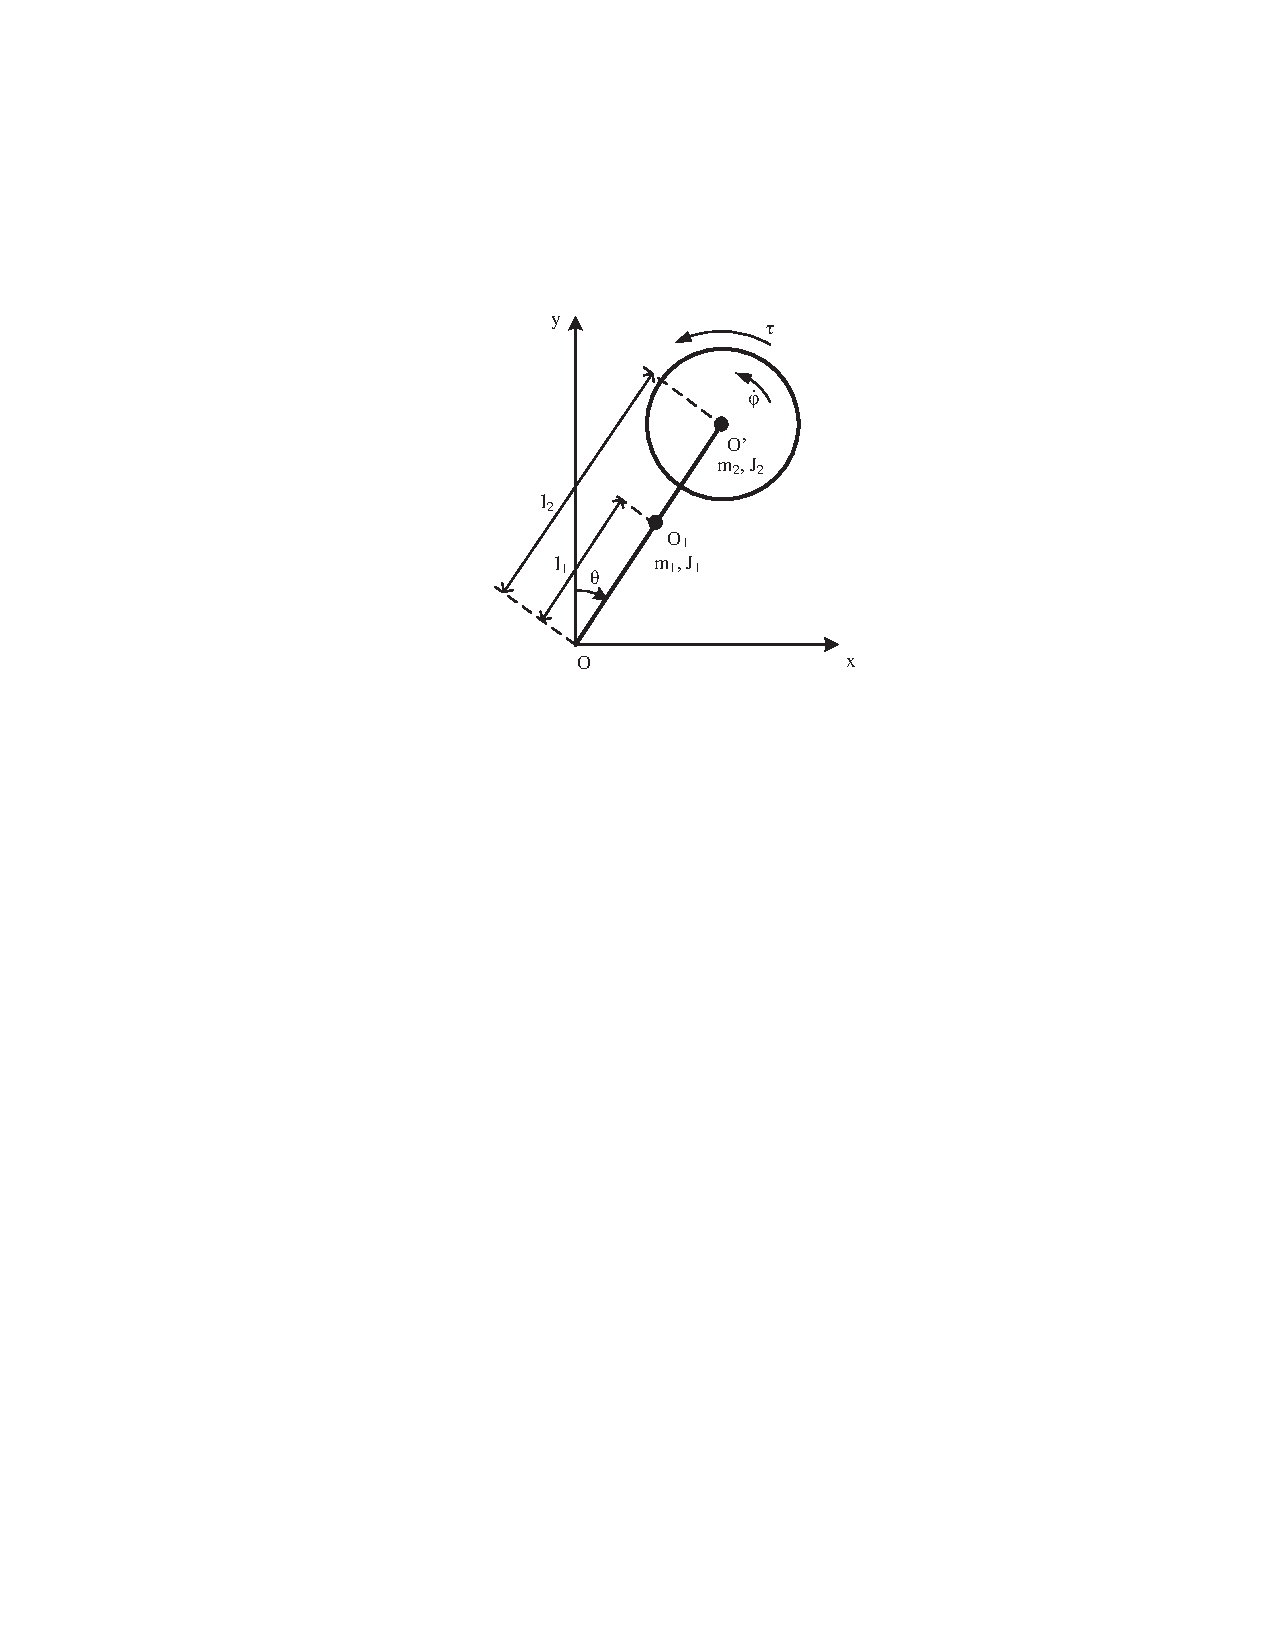
\includegraphics[width=0.4\textwidth]{Bilder/1. einfuehrung/Versuchsaufbau.pdf}}
   \caption[Modellskizze des Versuchs]{Modellskizze des Schwungrad-Pendel-Versuchs inklusive relevanter Modellparameter}
   \label{fig:Bild1.1}
\end{figure}

Weiterhin gelten folgende Voraussetzungen für das System:

\begin{itemize}
    \item Das Pendel ist frei gelagert.
    \item Der Motor (Gleichstrommaschine) ist spannungsgeregelt (bei $V_{\mathrm{m,Max}} = \SI{20}{V}$).
    \item Der Winkel ($\theta$) des Pendels und der Winkel ($\varphi$) des Schwungrades werden gemessen.
\end{itemize}

Es sind folgende Einschränkungen ermittelt/festgelegt worden:

\begin{itemize}
    \item Das Aufschwingen soll über eine schnelle Steuerung umgesetzt werden.
    \item Es soll ein Zustandsregler mit vier Zuständen ($x_{\mathrm{1}}$ bis $x_{\mathrm{4}}$) verwendet werden für die Regelung um die Ruhelage.
    \item Für die Ermittlung der Winkelgeschwindigkeiten ($\dot\theta$ und $\dot\varphi$) ist die Rekonstruktion über einen Beobachter notwendig.
\end{itemize}
\pagestyle{aaron}
\section{Modellierung des Schwungrad-Pendels} \label{sec:Modellierung}

Der folgende Abschnitt beschäftigt sich mit der Modellierung des Schwungrad-Pendels inklusive des treibenden Gleichstrommotors.

\subsection{Modellierung des Gleichstrommotors}

\begin{figure}[H]
    \centering
    \fbox{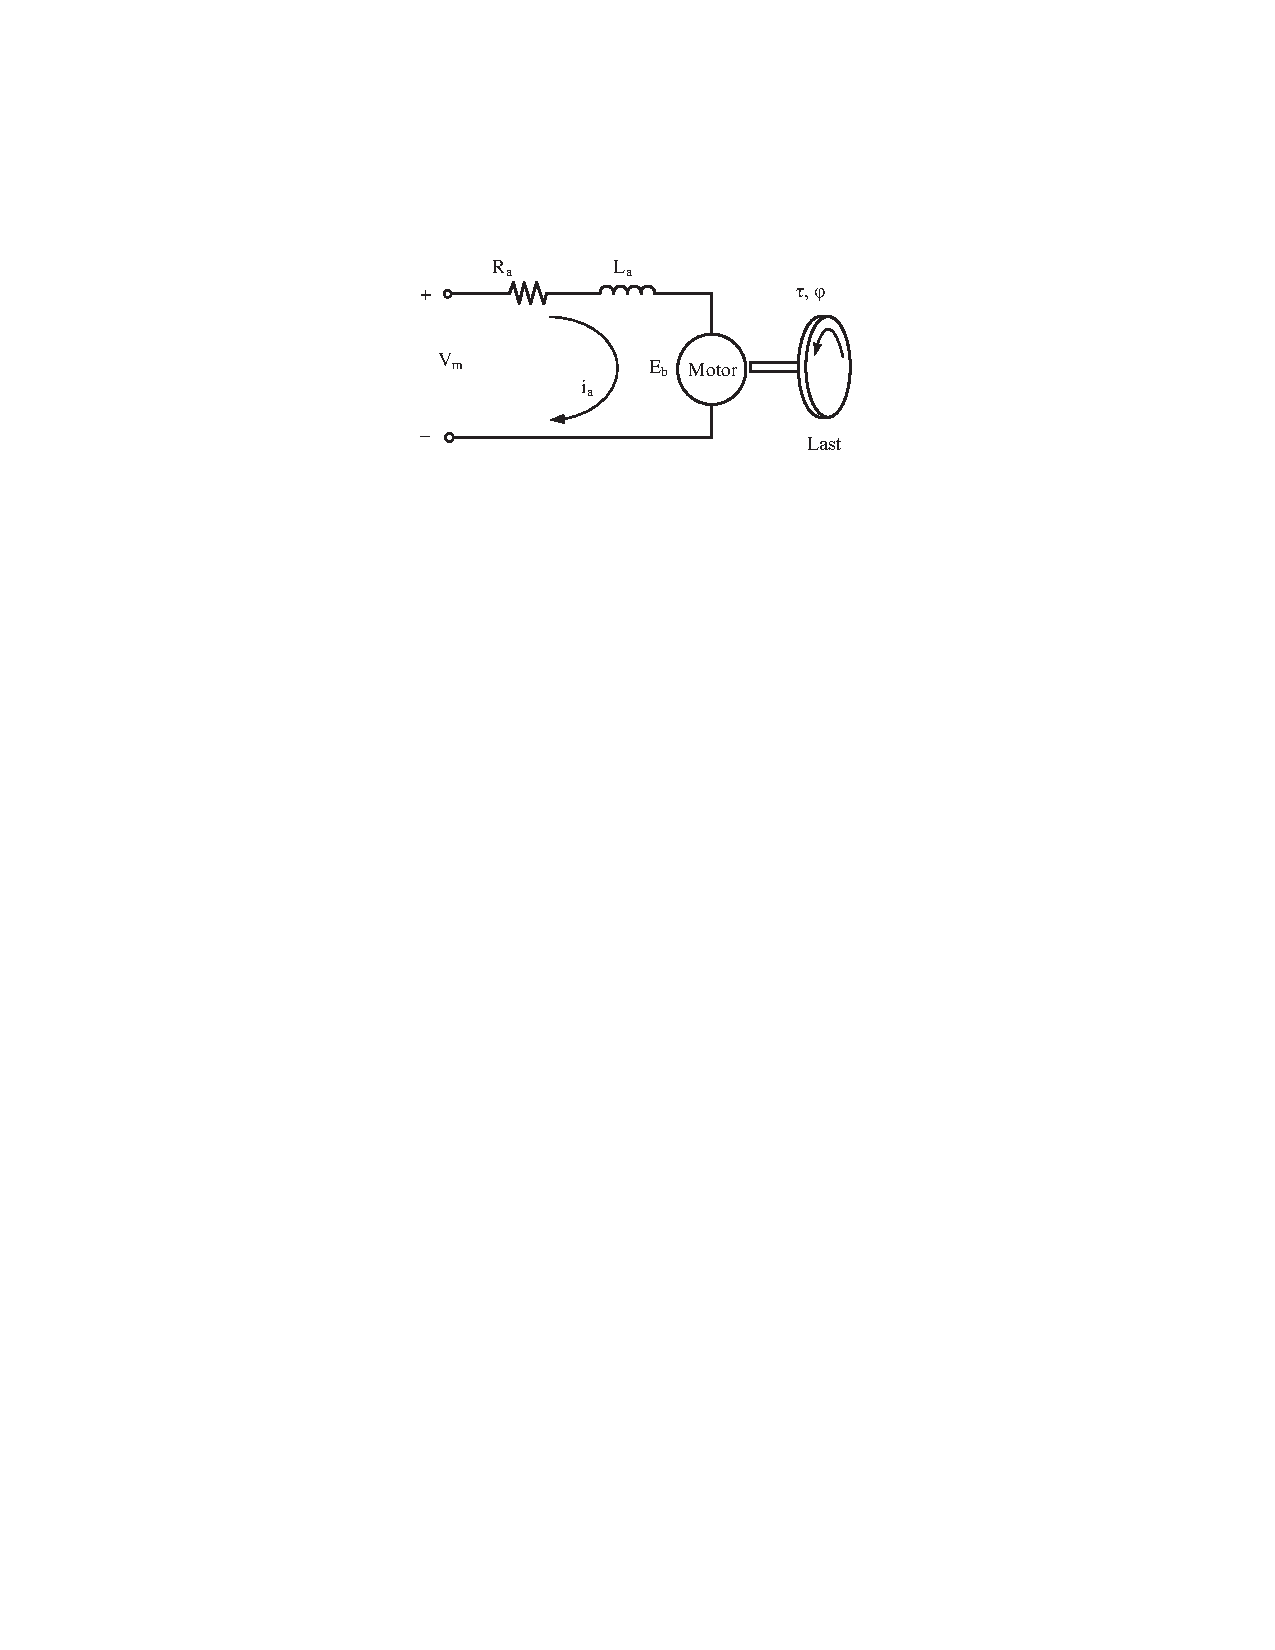
\includegraphics[width=0.6\textwidth]{Bilder/2_modellierung/Ersatzschaltbild.pdf}}
    \caption[Ersatzschaltbild Gleichstrommotor]{Ersatzschaltbild des Gleichstrommotors am Schwungrad-Pendel}
    \label{fig:Bild2.1}
\end{figure}

\autoref{fig:Bild2.1} zeigt das Ersatzschaltbild des Gleichstrommotors am Schwungrad-Pendel. Das zweite Kirchhoff'sche Gesetzt ergibt folgende Gleichung:

\begin{equation} \label{eq:Gleichung2.1}
    V_{\mathrm{m}} = i_{\mathrm{a}} R_{\mathrm{a}} + L_{\mathrm{a}} \frac{di_{\mathrm{a}}}{dt} + E_{\mathrm{b}}
\end{equation}
\newline
Die gegenelektromotorische Kraft (EMK) hängt von der Winkelgeschwindigkeit $\dot\varphi$ und der Gegen-EMK-Konstante $K_{\mathrm{b}}$ wie folgt ab:

\begin{equation} \label{eq:Gleichung2.2}
    E_{\mathrm{b}} = K_{\mathrm{b}} \dot\varphi
\end{equation}
\newline
Angenommen die Wirkung der Induktivität ist sehr klein ($L_{\mathrm{a}} \ll R_{\mathrm{a}}$), \autoref{eq:Gleichung2.1} ergibt sich zu

\begin{equation} \label{eq:Gleichung2.3}
    i_{\mathrm{a}} = \frac{V_{\mathrm{m}} - K_{\mathrm{b}} \dot\varphi}{R_{\mathrm{a}}}.
\end{equation}
\newline
Das Motordremoment $\tau$ ist mit dem Ankerstrom $i_{\mathrm{a}}$ durch eine Motordrehmomentkonstante $K_{\mathrm{t}}$ verbunden. Die Modellgleichung des Gleichstrommotors ergibt sich somit zu:

\begin{equation} \label{eq:Gleichung2.4}
    \boxed{\tau = K_{\mathrm{t}} i_{\mathrm{a}} = K_{\mathrm{t}} \frac{V_{\mathrm{m}} - K_{\mathrm{b}} \dot\varphi}{R_{\mathrm{a}}}}
\end{equation}

\subsection{Modellierung des Schwungrad-Pendels}

Zur Modellierung des Pendels wurde der Langrange-Ansatz gewählt, um die Bewegungsgleichungen des Pendels herzuleiten.
 
\subsubsection{Lagrange Ansatz}

Die nachfolgende Gleichung zeigt den \textbf{Lagrange Ansatz} unter Berücksichtigung der \textbf{dissipativen Funktion}. Diese besagt in Erweiterung zu der Lagrange-Formulierung, dass Energie in einem Vorgang in Wärme umgewandelt wird. Mit Hilfe der dissipativen Funktion können \textbf{Reibungsverluste} bei der Energiemethode nach Lagrange berücksichtigt werden.
\begin{equation} \label{eq:Gleichung2.5}
    \boxed{\frac{d}{dt} \left(\frac{\partial L}{\partial \dot{q_{\mathrm{i}}}}\right) - \frac{\partial L}{\partial q_{\mathrm{i}}} + \frac{\partial D}{\partial \dot{q_{\mathrm{i}}}} = 0}
\end{equation}

\subsubsection{Freiheitsgrade und Zwangsbedingungen}

In \autoref{fig:Bild1.1} sind zwei Teilchen \bzw Massepunkte im $\mathbb{R}^2$ zu erkennen. Zum Einen die des Pendels und zum Anderen die des Schwungrades. Somit gilt grundsätzlich:

\begin{itemize}
    \item 2 Punkte: 4 Freiheitsgrade (FHG)
\end{itemize}

Das Schwungrad-Pendel besitzt jedoch auch zwei Zwangsbedingungen, die wie folgt formuliert werden können:

\begin{itemize}
    \item Das Pendel kann nur um die 0z-Achse rotieren: \\ $z = 0$
    \item Die Masse $m_2$ ist über des Pendel mit dem Aufhängepunkt 0 gekoppelt: \\ $(y_{\mathrm{m_1}} - y_{\mathrm{m_2}})^2 + (x_{\mathrm{m_1}} - x_{\mathrm{m_2}})^2 = l_2^2$
\end{itemize}

Beide Zwangsbedingungen sind holonom-skleronom, da sie als Gleichungen zwischen zwei Koordinaten angegeben werden können und nicht von der Zeit abhängig sind.

Somit bleiben am Ende noch zwei Freiheitsgrade (FHG) übrig.

\subsubsection{Generalisierte Koordinaten}

Aus den verbliebenen Freiheitsgraden werden die generalisierten Koordinaten abgeleitet. Dabei gilt grundsätzlich folgender Zusammenhang im $\mathbb{R}^2$:

\begin{equation} \label{eq:Gleichung2.6}
    \boxed{S = 2n - k}
\end{equation}
\newline
mit $S$ als Anzahl der Freiheitsgrade und somit auch der Anzahl der generalisierten Koordinaten, $n$ der Anzahl der Teilchen und $k$ der Anzahl der holonomen Zwangsbedingungen.\\
Die beiden Generalisierten Koordinaten sind somit:

\begin{itemize}
    \item $q_{\mathrm{1}} = \theta$
    \item $q_{\mathrm{2}} = \varphi$
\end{itemize}

\subsubsection{Berechnung der kinetischen und potentiellen Energie}

Für die Lagrange-Formulierung werden die kinetische und die potentielle Energie des Systems benötigt. Die kinetische Energie setzt sich zusammen aus der translatorischen kinetischen Energie $E_{\mathrm{kin,trans}}$ und der rotatorischen kinetischen Energie $E_{\mathrm{kin,rot}}$. Die Gleichungen sind nachfolgend aufgestellt.

\begin{align} \label{eq:Gleichung2.7}
    \begin{split}
        E_{\mathrm{kin,trans}} &= \frac{1}{2} m_1 (l_1\dot\theta)^2 + \frac{1}{2}m_2 (l_2\dot\theta)^2 \\
        E_{\mathrm{kin,rot}} &= \frac{1}{2} J_1 (\dot\theta)^2 + \frac{1}{2} J_2 (\dot\theta + \dot\varphi)^2
    \end{split}
\end{align}
\newline
Die gesamte \textbf{kinetische Energie des Systems} ist somit:

\begin{empheq}[box=\widefbox]{align} \label{eq:Gleichung2.8}
    \begin{split}
        E_{\mathrm{kin}} &= E_{\mathrm{kin,trans}} + E_{\mathrm{kin,rot}} \\
        E_{\mathrm{kin}} &= \frac{1}{2} \left( m_1 l_1^2 + m_2 l_2^2 + J_1 + J_2 \right) \dot\theta^2 + J_2\dot\theta\dot\varphi + \frac{1}{2} J_2 \dot\varphi^2
    \end{split}
\end{empheq}
\newline
Der Ursprung der potentiellen Energie liegt bei Null. Somit ergibt sich die \textbf{potentielle Energie des Systems} zu:

\begin{equation} \label{eq:Gleichung2.9}
    \boxed{E_{\mathrm{pot}} = \left( m_1 l_1 + m_2 l_2 \right) g\cos (\theta)}
\end{equation}

\subsubsection{Herleitung der Bewegungsgleichungen}

Die \textbf{Lagrange-Funktion} $L$ wird aus der Differenz der kinetischen Energie aus \autoref{eq:Gleichung2.8} und der potentiellen Energie aus \autoref{eq:Gleichung2.9} berechnet.

\begin{empheq}[box=\widefbox]{align} \label{eq:Gleichung2.10}
    \begin{split}
        L &= E_{\mathrm{kin}} - E_{\mathrm{pot}} \\
        L &= \frac{1}{2} \left( m_1 l_1^2 + m_2 l_2^2 + J_1 + J_2 \right) \dot\theta^2 + J_2\dot\theta\dot\varphi + \frac{1}{2} J_2 \dot\varphi^2 - \left( m_1 l_1 + m_2 l_2 \right) g\cos (\theta)
    \end{split}
\end{empheq}
\newline
Die \textbf{dissipative Energie} $D$ ist:

\begin{equation} \label{eq:Gleichung2.11}
    \boxed{D = \frac{1}{2} c_1 \dot\theta^2 + \frac{1}{2} c_2 \dot\varphi^2}
\end{equation}
\newline
Zieht man nun den Ansatz aus \autoref{eq:Gleichung2.5} heran und wendet diesen für die generalisierte Koordinate $\theta$ an, so erhält man die \textbf{Bewegungsgleichung des Schwungrades}:

\begin{equation} \label{eq:Gleichung2.12}
    \boxed{\left( m_1 l_1^2 + m_2 l_2^2 + J_1 + J_2\right) \ddot\theta + J_2\ddot\varphi + c_1\dot\theta - \left( m_1 l_1 + m_2 l_2 \right) g\sin (\theta) = 0}
\end{equation}
\newline
Ebenfalls der Gleiche Ansatz wird nun für die generalisierte Koordinate $\varphi$ angewendet:

\begin{equation} \label{eq:Gleichung2.13}
    J_2 \left( \ddot\theta + \ddot\varphi \right) + c_2 \dot\varphi = \tau
\end{equation}
\newline
Setzt man nun \autoref{eq:Gleichung2.4} in \autoref{eq:Gleichung2.13} ein erhält man die \textbf{Bewegungsgleichung des Pendels}:

\begin{equation} \label{eq:Gleichung2.14}
    \boxed{J_2 \left( \ddot\theta + \ddot\varphi \right) + c_2 \dot\varphi = K_{\mathrm{t}} i_{\mathrm{a}} = K_{\mathrm{t}} \frac{V_{\mathrm{m}} - K_{\mathrm{b}} \dot\varphi}{R_{\mathrm{a}}}}
\end{equation}
\pagestyle{aaron}
\section{Zustandsraumdarstellung} \label{sec:Zustandsraumdarstellung}

Um das Verhalten mittels mathematischer Beziehungen zu veranschaulichen, wird die \textbf{Zustandsraumdarstellung} verwendet. Der \textbf{Systemeingang} wird festgelegt mit

\begin{equation} \label{eq:Gleichung3.1}
    \underline{u} = V_{\mathrm{m}},
\end{equation}
\newline
wobei $V_{\mathrm{m}}$ die Eingangsspannung des Gleichstrommotors aus \autoref{eq:Gleichung2.1} ist.Die \textbf{Systemzustände} des Schwungrad-Pendels sind:

\begin{align}
    \underline{x} &=
    \begin{bmatrix} \label{eq:Gleichung3.2}
        x_{\mathrm{1}} \\
        x_{\mathrm{2}} \\
        x_{\mathrm{3}} \\
        x_{\mathrm{4}}
    \end{bmatrix} =
    \begin{bmatrix}
        \varphi     \\
        \dot\varphi \\
        \theta      \\
        \dot\theta
    \end{bmatrix}
\end{align}
\newline
Nach zeitlicher Ableitung des Zustandsvektors ergibt sich der \textbf{Vektor der Zustandsänderung} zu:

\begin{align}
    \underline{x} &=
    \begin{bmatrix} \label{eq:Gleichung3.3}
        \dot x_{\mathrm{1}} \\
        \dot x_{\mathrm{2}} \\
        \dot x_{\mathrm{3}} \\
        \dot x_{\mathrm{4}}
    \end{bmatrix} =
    \begin{bmatrix}
        \dot\varphi     \\
        \ddot\varphi    \\
        \dot\theta      \\
        \ddot\theta
    \end{bmatrix}
\end{align}
\newline
Die \textbf{Ausgänge des Systems} gleichen den den vier Zuständen und ergeben sich somit zu

\begin{align}
    \underline{y} &=
    \begin{bmatrix} \label{eq:Gleichung3.4}
        \varphi     \\
        \dot\varphi \\
        \theta      \\
        \dot\theta
    \end{bmatrix}.
\end{align}

\subsection{Nichtlineares Zustandsraummodell}\label{cap:nichtlinearesZustandsraummodell}

Zum Aufstellen des nichtlinearen Zustandsraummodells werden die \autoref{eq:Gleichung2.12} und \autoref{eq:Gleichung2.14} nach den höchsten Ableitungen von $\ddot\varphi$ und $\ddot\theta$ umgestellt.

\begin{align} \label{eq:Gleichung3.5}
    \begin{split}
        \ddot\varphi &= \frac{K_{\mathrm{t}} \frac{V_{\mathrm{m}} - K_{\mathrm{b}} \dot\varphi}{R_{\mathrm{a}}} - c_2 \dot\varphi - J_2 \cdot \ddot\theta}{J_2} \\
        \ddot\theta &= \frac{-J_2 \ddot\varphi - c_1 \dot\theta + \left( m_1 l_1 + m_2 l_2\right) g \sin(\theta)}{m_1 l_1^2 + m_2 l_2^2 + J_1 + J_2}
    \end{split}
\end{align}
\newline
Beide Gleichungen sind über die die Winkelbeschleunigung des Schwungrades $\ddot\varphi$ und die des Pendels $\ddot\theta$ miteinander verkoppelt. Durch das gegenseitige ineinander Einsetzen werden die Abhängigkeiten eliminiert.

\begin{align} \label{eq:Gleichung3.6}
    \begin{split}
        \ddot\varphi &= \frac{K_{\mathrm{t}} \frac{V_{\mathrm{m}} - K_{\mathrm{b}} \dot\varphi}{R_{\mathrm{a}}} - c_2 \dot\varphi - J_2 \cdot \left( \frac{-J_2 \ddot\varphi - c_1 \dot\theta + \left( m_1 l_1 + m_2 l_2\right) g \sin(\theta)}{m_1 l_1^2 + m_2 l_2^2 + J_1 + J_2}\right)}{J_2} \\
        \ddot\theta &= \frac{-J_2 \left( \frac{K_{\mathrm{t}} \frac{V_{\mathrm{m}} - K_{\mathrm{b}} \dot\varphi}{R_{\mathrm{a}}} - c_2 \dot\varphi - J_2 \cdot \ddot\theta}{J_2}\right) - c_1 \dot\theta + \left( m_1 l_1 + m_2 l_2\right) g \sin(\theta)}{m_1 l_1^2 + m_2 l_2^2 + J_1 + J_2}
    \end{split}
\end{align}
\newline
Mit Hilfe der Gleichungen \ref{eq:Gleichung3.1}, \ref{eq:Gleichung3.2} und \ref{eq:Gleichung3.3}, durch das einsetzen in \autoref{eq:Gleichung3.6} und dem Zusammenfassen und Umstellen nach $\ddot\varphi$ \bzw $\ddot\theta$ folgt das \textbf{nichtlineare Zustandsraummodell}.

\begin{empheq}[box=\widefbox]{align} \label{eq:Gleichung3.7}
    \underline{\dot x} =
    \begin{bmatrix}
        x_{\mathrm{2}} \\
        \frac{\frac{K_{\mathrm{t}} \cdot \frac{V_{\mathrm{m}} - K_{\mathrm{b}} \cdot x_4}{R_{\mathrm{a}}} - c_2 \cdot x_4 - \left( m_1 l_1 + m_2 l_2\right) g\sin(x_1) + c_1 \cdot x_2}{J_2}}{1 - \frac{m_1 l_1^2 + m_2 l_2^2 + J_1 + J_2}{J_2}} \\
        x_{\mathrm{4}} \\
        \frac{\frac{\left( m_1 l_1 + m_2 l_2\right) g\sin(x_1) - c_1 \cdot x_2 - \left( m_1 l_1^2 + m_2 l_2^2 + J_1 + J_2\right) \cdot \frac{K_{\mathrm{t}} \cdot \frac{V_{\mathrm{m}} - K_{\mathrm{b}} \cdot x_4}{R_{\mathrm{a}}}}{J_2}}{J_2}}{1 - \frac{m_1 l_1^2 + m_2 l_2^2 + J_1 + J_2}{J_2}}
    \end{bmatrix}
\end{empheq}

\subsection{Lineares Zustandsraummodell}

Das Verhalten des nichtlinearen Systems ist für große Änderungen des Eingangssignals nicht vorhersehbar. Um dennoch Aussagen über das Systemverhalten treffen zu können, wird das nichtlineare Zustandsraummodell mithilfe der Taylorreihenentwicklung um eine Ruhelage ($\underline{x}^{*}$) linearisiert. Die nichtlinearen Restglieder $\underline{R}(\Delta{\underline{x}^2}, \Delta{\underline{u}^2})$ werden zu Null angenommen. Durch die Linearisierung wird das Systemverhalten für kleine Änderungen um die Ruhelage kontrollierbar. Nachfolgend ist die Taylorreihenentwicklung für Linearisierung aufgeführt:

\begin{align} \label{eq:Gleichung3.8}
    \begin{split}
        \dot{\underline{x}}^{*}+\Delta{\dot{\underline{x}}} &=\underline{f}(\underline{x}^{*}+\Delta{\underline{x}},\underline{u}^{*}+\Delta{\underline{u}}) \\
        &=\underline{f}(\underline{x}^{*},\underline{u}^{*})+\left[\frac{\partial f_{\mathrm{i}}}{\partial x_{\mathrm{j}}}\right]_{(\underline{x}^{*}, \underline{u}^{*})}\cdot\Delta{\underline{x}}+\left[\frac{\partial f_{\mathrm{i}}}{\partial u_{\mathrm{j}}}\right]_{(\underline{x}^{*},\underline{u}^{*})}\cdot\Delta{\underline{u}}+\underline{R}(\Delta{\underline{x}^2}, \Delta{\underline{u}^2})
    \end{split}
\end{align}
\newline
Durch die Annahme über das Verhalten der nichtlinearen Restglieder folgt die Struktur des linearen Zustandsraummodells dargestellt in \autoref{eq:Gleichung3.9}.

\begin{align} \label{eq:Gleichung3.9}
    \begin{split}
        \Delta\dot{\underline{x}} &= \left[\frac{\partial f_{\mathrm{i}}}{\partial x_{\mathrm{j}}}\right]_{(\underline{x}^{*}, \underline{u}^{*})}\cdot\Delta{\underline{x}}+\left[\frac{\partial f_{\mathrm{i}}}{\partial u_{\mathrm{j}}}\right]_{(\underline{x}^{*},\underline{u}^{*})}\cdot\Delta{\underline{u}} \\   
        \Delta{\underline{y}} &= \left[\frac{\partial h_{\mathrm{i}}}{\partial x_{\mathrm{j}}}\right]_{(\underline{x}^{*}, \underline{u}^{*})}\cdot\Delta{\underline{x}}+\left[\frac{\partial h_{\mathrm{i}}}{\partial u_{\mathrm{j}}}\right]_{(\underline{x}^{*},\underline{u}^{*})}\cdot\Delta{\underline{u}}
    \end{split}
\end{align}
\newline
Um das linearisierte Zustandsraummodell zu erhalten, werden die einzelnen Gleichungen des nichtlinearen Zustandsraummodells aus \autoref{eq:Gleichung3.7} nach den Zuständen $x_{\mathrm{1}}$ bis $x_{\mathrm{4}}$, sowie dem Eingang $V_{\mathrm{m}}$ partiell abgeleitet und die Ruhelage $\underline{x}^{*}$ eingesetzt. Dabei werden sowohl die Ruhelage des hängenden Pendels (untere Ruhelage) und die des stehenden Pendels (obere Ruhelage) betrachtet. In \autoref{eq:Gleichung3.10} dargestellt ist die untere Ruhelage, mit Hilfe derer das lineare Zustandsraummodell für das hängende Pendel bestimmt werden kann. Anhand dessen kann das lineare Zustandsraummodell in Simulink mit dem nichtlinearen Zustandsraummodell im nachfolgenden Abschnitt (\autoref{sec:Vergleich}) verglichen werden.

\begin{align}\label{eq:Gleichung3.10}
    \begin{split}
        \underline{x}_{\mathrm{1}}^{*}=
        \begin{bmatrix}
            x_{\mathrm{1}}^{*} \\
            x_{\mathrm{2}}^{*} \\
            x_{\mathrm{3}}^{*} \\
            x_{\mathrm{4}}^{*}
        \end{bmatrix}=
        \begin{bmatrix}
            \pi \\
            0   \\
            0   \\
            0
        \end{bmatrix}
    \end{split}
\end{align}
\newline
Die Regelung, welche in \autoref{sec:Zustandsregler} entworfen wird soll dafür sorgen, dass das Pendel in der oberen Ruhelage verweilt. Diese wird beschrieben durch:

\begin{align}\label{eq:Gleichung3.11}
    \begin{split}
        \underline{x}_{\mathrm{2}}^{*}=
        \begin{bmatrix}
            x_{\mathrm{1}}^{*} \\
            x_{\mathrm{2}}^{*} \\
            x_{\mathrm{3}}^{*} \\
            x_{\mathrm{4}}^{*}
        \end{bmatrix}=
        \begin{bmatrix}
            0 \\
            0 \\
            0 \\
            0
        \end{bmatrix}
    \end{split}
\end{align}
\newline
Die allgemeine Form des \textbf{linearen Zustandsraummodells} lautet:

\begin{empheq}[box=\widefbox]{align} \label{eq:Gleichung3.12}
    \begin{split}
        \dot{\underline{x}} &= \underline{A}\cdot\underline{x}+\underline{B}\cdot\underline{u} \\
        \underline{y} &= \underline{C}\cdot\underline{x}+\underline{D}\cdot\underline{u}
    \end{split}
\end{empheq}
\newline
Wendet man nun die Linearisierungsvorschrift aus \autoref{eq:Gleichung3.9} unter Nutzung der Ruhelagen an, so erhält man das konkrete linearisierte Zustandsraummodell für das System. In \autoref{eq:Gleichung3.13} ist das linearisierte Zustandsraummodell für die obere Ruhelage und in \autoref{eq:Gleichung3.14} das für die untere Ruhelage dargestellt.

\begin{empheq}[box=\widefbox]{align} \label{eq:Gleichung3.13}
    \begin{split}
        \Delta{\dot{\underline{x}}}&=
        \begin{bmatrix}
            0           & 1         & 0 & 0         \\
            -50.9760    & -1.2328   & 0 & 0.1960    \\
            0           & 0         & 0 & 1         \\
            50.9760     & 1.2328    & 0 & -11.3323
        \end{bmatrix}\cdot\Delta\underline{x}+
        \begin{bmatrix}
            0       \\
            -1.9548 \\
            0       \\
            113.0101
        \end{bmatrix}\cdot V_{\mathrm{m}}
        \\
        \Delta{\underline{y}} &=
        \begin{bmatrix}
            1 & 0 & 0 & 0 \\
            0 & 0 & 1 & 0
        \end{bmatrix}\cdot\Delta\underline{x}+\underline{0}\cdot V_{\mathrm{m}}
    \end{split}
\end{empheq}

\begin{empheq}[box=\widefbox]{align} \label{eq:Gleichung3.14}
    \begin{split}
        \Delta{\dot{\underline{x}}}&=
        \begin{bmatrix}
            0           & 1         & 0 & 0         \\
            50.9760     & -1.2328   & 0 & 0.1960    \\
            0           & 0         & 0 & 1         \\
            -50.9760    & 1.2328    & 0 & -11.3323
        \end{bmatrix}\cdot\Delta\underline{x}+
        \begin{bmatrix}
            0       \\
            -1.9548 \\
            0       \\
            113.0101
        \end{bmatrix}\cdot V_{\mathrm{m}}
        \\
        \Delta{\underline{y}} &=
        \begin{bmatrix}
            1 & 0 & 0 & 0 \\
            0 & 0 & 1 & 0
        \end{bmatrix}\cdot\Delta\underline{x}+\underline{0}\cdot V_{\mathrm{m}}
    \end{split}
\end{empheq}
\pagestyle{aaron}
\section{Vergleich lineares/nichtlineares System} \label{sec:Vergleich}

In \autoref{fig:Bild4.1} ist die Übersicht der notwendigen Simulationsstruktur dargestellt. Aus der Übersicht geht hervor, dass beide Systeme unterschiedliche Eingänge besitzen und somit ein direkter Vergleich ohne entsprechende Berücksichtigung der Linearisierungsvorschriften unmöglich ist. Das linearisierte Modell verwendet als Eingang im Gegensatz zum nichtlinearen Modell eine Differenz $\Delta u$. Die Strukturen des nichtlinearen und des linearen Modells sind zur Information in \autoref{fig:Bild4.2} und \autoref{fig:Bild4.3} visualisiert.

\begin{figure}[H]
   \centering
   \fbox{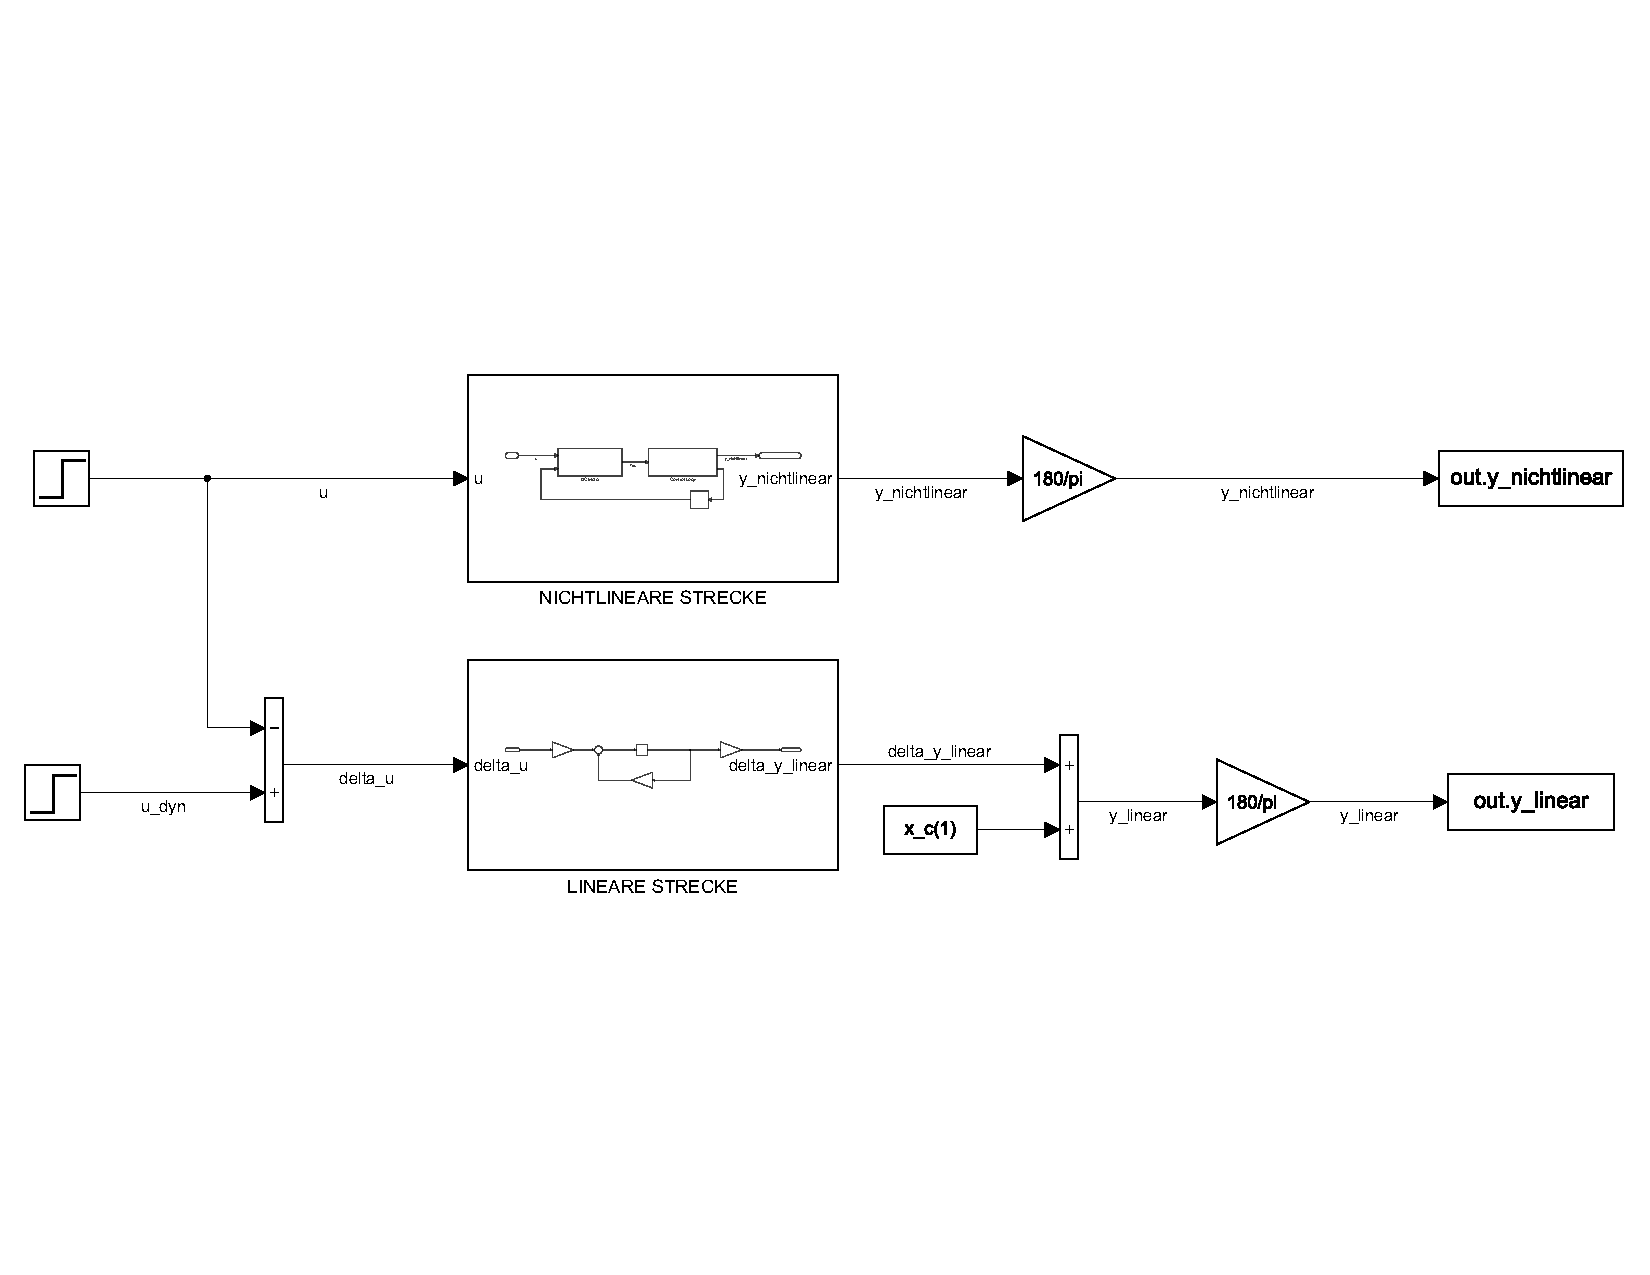
\includegraphics[width=0.65\textwidth]{Bilder/4. vergleich/system.pdf}}
   \caption[Übersicht der Simulationsstruktur]{Übersicht der Simulationsstruktur}
   \label{fig:Bild4.1}
\end{figure}

\begin{figure}[H]
   \centering
   \fbox{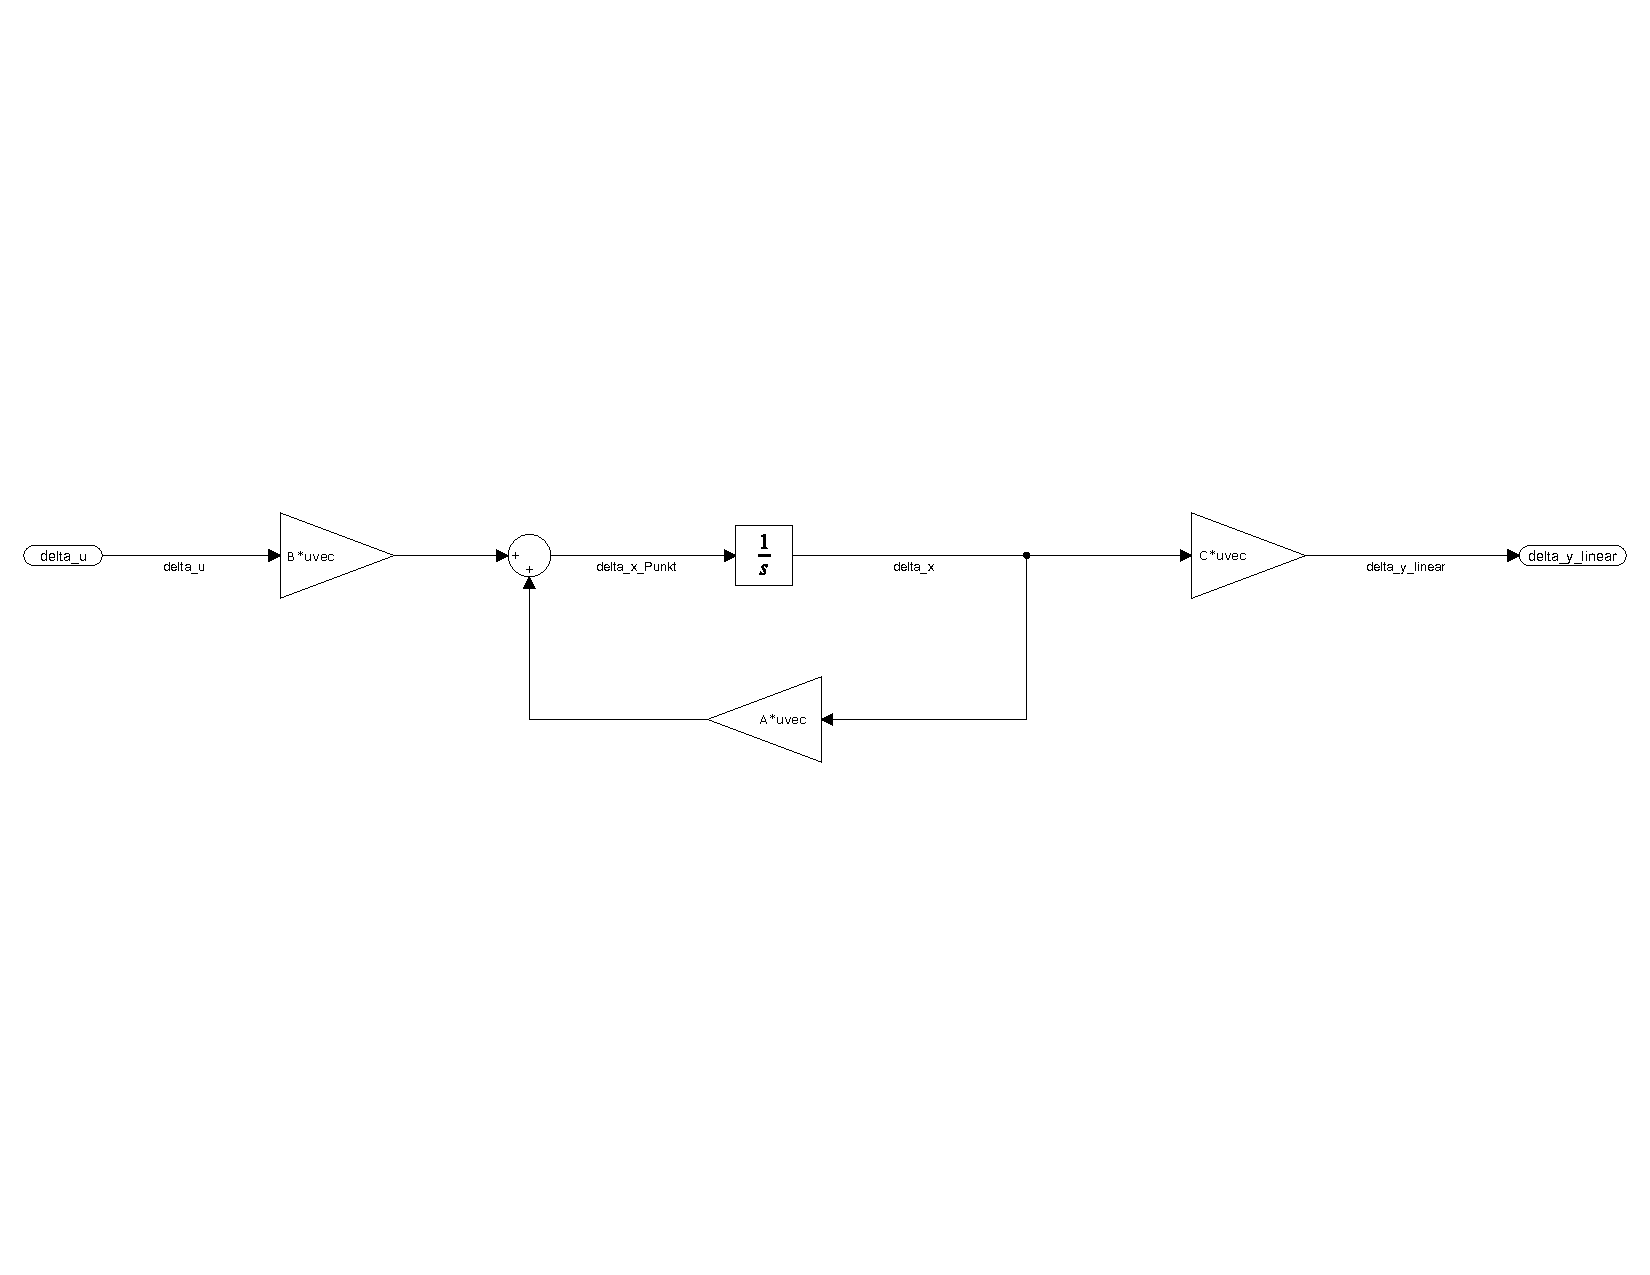
\includegraphics[width=0.65\textwidth]{Bilder/4. vergleich/linear.pdf}}
   \caption[Nichtlineare Strecke]{Nichtlineare Strecke}
   \label{fig:Bild4.2}
\end{figure}

\begin{figure}[H]
   \centering
   \fbox{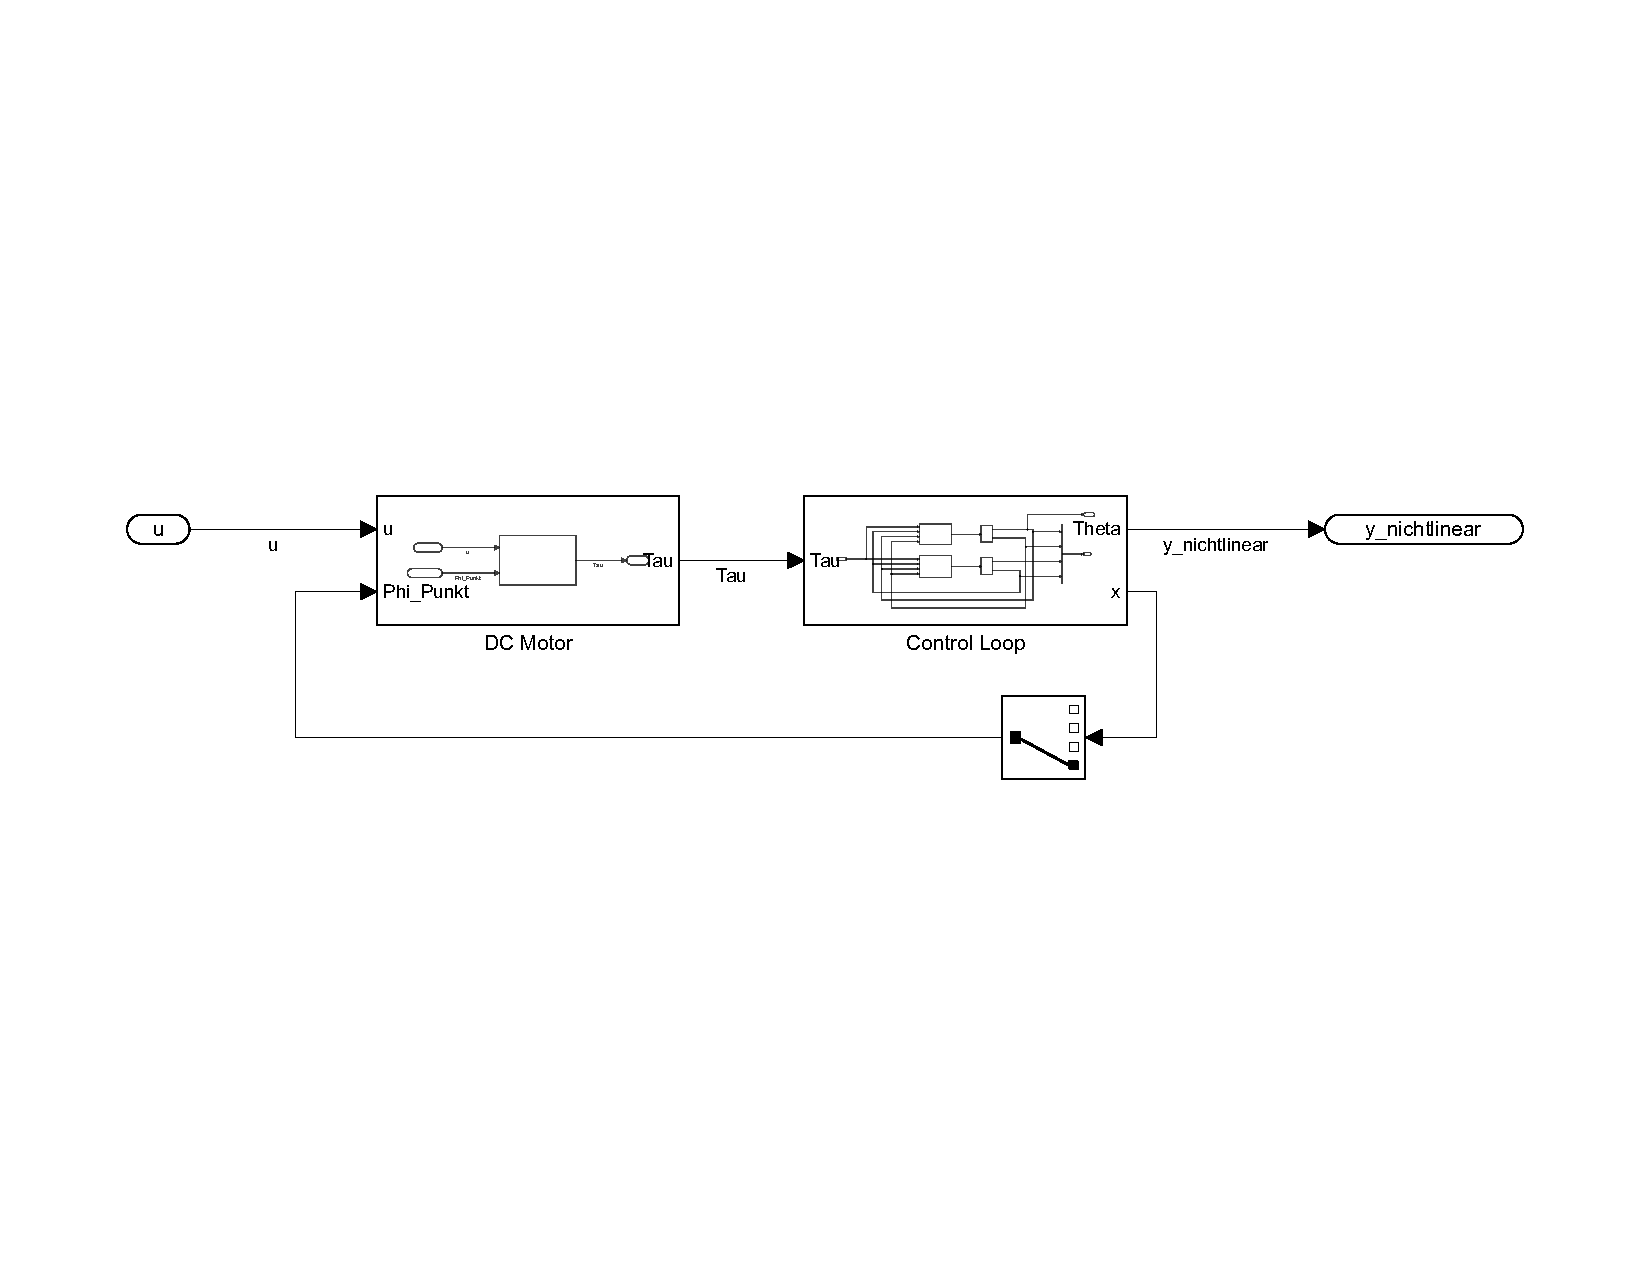
\includegraphics[width=0.65\textwidth]{Bilder/4. vergleich/nichtlinear.pdf}}
   \caption[Lineare Strecke]{Lineare Strecke}
   \label{fig:Bild4.3}
\end{figure}

Um das lineare mit dem nichtlinearen Modell zu vergleichen, werden gemäß \autoref{sec:Zustandsraumdarstellung} zu den Zuständen $\Delta \underline{x}$ die Ruhelagen $\underline{x}^*$ aus \autoref{eq:Gleichung3.10} addiert. Aus der \autoref{fig:Bild4.4} und \autoref{fig:Bild4.5} geht hervor, dass die implementierten Systeme für kleine Abweichungen von der Ruhelagen mit steigender Zeit $"t"$ selbiges Verhalten aufweisen.

\begin{figure}[H]
   \centering
   \fbox{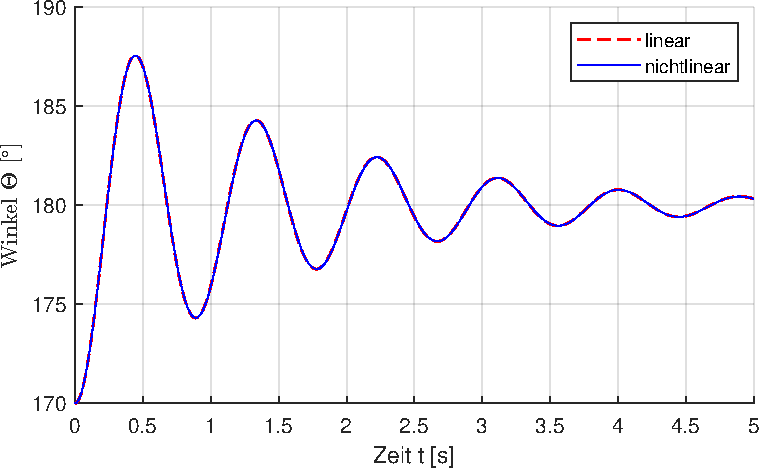
\includegraphics[width=0.7\textwidth]{Bilder/4. vergleich/vergleich_10_grad.pdf}}
   \caption[Vergleich der Pendelwinkel $\theta$ - kleine Auslenkung]{Vergleich der Pendelwinkel $\theta$ bei -10${^\circ}$ Anfangsauslenkung zur Ruhelage}
   \label{fig:Bild4.4}
\end{figure}

\begin{figure}[H]
   \centering
   \fbox{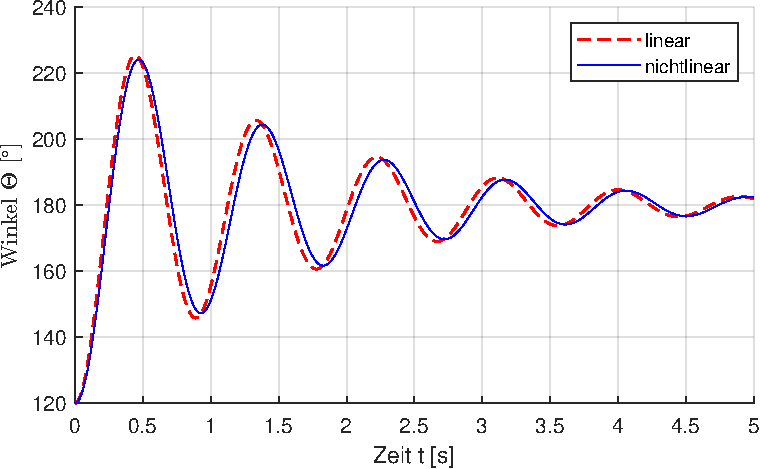
\includegraphics[width=0.7\textwidth]{Bilder/4. vergleich/vergleich_60_grad.pdf}}
   \caption[Vergleich der Pendelwinkel $\theta$ - große Auslenkung]{Vergleich der Pendelwinkel $\theta$ bei -60${^\circ}$ Anfangsauslenkung zur Ruhelage}
   \label{fig:Bild4.5}
\end{figure}
\pagestyle{milan}
\section{Sensitivitätsanalyse der Modellparameter}\label{sec:sesitivitaetsanalyse}
In diesem Abschnitt wird eine Parameter- und Sensivitätsanalysise durchgeführt. 
Es wird dabei die Auswirkung von der Varianz von bestimmten Modellparametern auf die Varianz der Ausgangsparameter untersucht.

Ziel der Sensitivitätsanalyse ist es, wichtige Parameter zu identifizieren und daraus eine Optimierung der Parameter zu ermitteln.

Das Ergebniss der Sensitivitätsanalyse dient zum weiterne Verständnis des mathematischen Modelles bzw. dem zugrundeliegenden Simulationsmodell.
\subsection{Lokale und globlale Sensitivitätsanalyse}

Die verschiedenen Verfahren zur Sensitivitätsanalyse lassen sich in drei Kategorien einteilen: Lokale, globale Sensitivitätsanalyse und der sogenannenten Screening Methode.

Bei der lokalen Sensitivitätsanalyse wird für bestimmte Werte der Ausgnagsgrößen der Einfluss der Eingangsgrößen untersucht. Dabei wird immer ein Parameter variiert und die restlichen konstant gehalten (One-At-a-Time-Methode, OAT).
Die Sensitivitätsanalyse wird so für jeden Parameter einzeln durchgeführt und abschließend kann die spezifische Sensivität der einzelnen Parameter ermittelt werden.
Mathematisch entspricht dies den partiellen Ableitungen der Parameter bezüglich der Ausgangsgrößen

\subsubsection*{One-factor-at-a-time ($\pm \SI{20}{\percent}, \pm 1\, \sigma$)}

\begin{equation}
    sensitivity=\frac{\Delta Y}{\Delta X_{i}} \quad \textrm{Für jeden Parameter}\,X_i, i=1,\dots,n
\end{equation}
\begin{itemize}
    \item Nur lokale Variatizion um Arbeitspunk 
    \item Keine Korrelation zwischen Parametern
    \item Standartabweichung benötigt Annahme zur Distribution und überspannt nicht den gesammten Wertebereich
\end{itemize}

\subsubsection*{Ausdruck als Partial-Ableitung}
\begin{equation}
    sensitivity=\frac{\partial Y}{\partial X_i}
\end{equation}

%\begin{figure}   
%    % This file was created by matlab2tikz.
%
%The latest updates can be retrieved from
%  http://www.mathworks.com/matlabcentral/fileexchange/22022-matlab2tikz-matlab2tikz
%where you can also make suggestions and rate matlab2tikz.
%
\definecolor{mycolor1}{rgb}{0.00000,0.44700,0.74100}%
%
\begin{tikzpicture}

\begin{axis}[%
    %title={{$\dot\varphi\, t_{Settle}$}},
    %axis lines = left,
    xlabel = {$V_{m}\,[V]$},
    y label style={at={(axis description cs:0.3,1)},rotate=-90,anchor=south},
    ylabel = {$t_{\dot\varphi}\, [s]$},
    xmin=0,
    xmax=20,
    xtick={0,5,10,15,20},
    %ytick={0.380,0.381,0.382,0.383,0.384},
    ymajorgrids=true,
    xmajorgrids=true,
    grid style=dashed,
    y tick label style={
        /pgf/number format/.cd,
            %fixed,
           % fixed zerofill,
            precision=4,
        /tikz/.cd
    },
]
\addplot [color=mycolor1, only marks, mark size=0.5pt, mark=*, mark options={solid, black}, forget plot]
  table[row sep=crcr]{%
2.80511	0.38325\\
5.20260	0.38324\\
1.73630	0.38325\\
8.58795	0.38321\\
5.14566	0.38324\\
5.95111	0.38323\\
8.49717	0.38321\\
2.38415	0.38325\\
9.90134	0.38319\\
14.12814	0.38312\\
4.87147	0.38324\\
15.70140	0.38309\\
1.48179	0.38325\\
7.87767	0.38321\\
0.06788	0.38326\\
4.41354	0.38324\\
0.02601	0.38326\\
3.78359	0.38325\\
2.84968	0.38325\\
5.36152	0.38324\\
3.49784	0.38325\\
2.77298	0.38325\\
11.97771	0.38316\\
18.02116	0.38303\\
18.78760	0.38301\\
4.42369	0.38324\\
9.65343	0.38319\\
7.52022	0.38322\\
10.47560	0.38318\\
5.29745	0.38324\\
1.36714	0.38325\\
8.72654	0.38320\\
3.47706	0.38325\\
0.52214	0.38326\\
19.09357	0.38300\\
8.61193	0.38321\\
19.23117	0.38300\\
15.24829	0.38310\\
0.14697	0.38326\\
13.60077	0.38313\\
14.11902	0.38312\\
12.90258	0.38314\\
11.04620	0.38317\\
4.36217	0.38324\\
15.44732	0.38309\\
4.56057	0.38324\\
7.41729	0.38322\\
17.81858	0.38303\\
17.12754	0.38305\\
8.04867	0.38321\\
6.36038	0.38323\\
12.17271	0.38316\\
18.20390	0.38302\\
18.18196	0.38303\\
11.83189	0.38316\\
6.65143	0.38323\\
17.06127	0.38305\\
8.84796	0.38320\\
18.08711	0.38303\\
0.66359	0.38326\\
10.64853	0.38318\\
14.32995	0.38312\\
3.58604	0.38325\\
6.73066	0.38323\\
3.75426	0.38325\\
6.43854	0.38323\\
8.07713	0.38321\\
10.97133	0.38317\\
0.97477	0.38326\\
11.05464	0.38317\\
5.49623	0.38324\\
4.83003	0.38324\\
4.86290	0.38324\\
3.08319	0.38325\\
19.12833	0.38300\\
18.71323	0.38301\\
16.37429	0.38307\\
14.56524	0.38311\\
3.51623	0.38325\\
7.20742	0.38322\\
3.77580	0.38325\\
0.02397	0.38326\\
6.32839	0.38323\\
13.99234	0.38312\\
12.50510	0.38315\\
10.86124	0.38318\\
8.78074	0.38320\\
5.74855	0.38323\\
10.03318	0.38319\\
15.23092	0.38310\\
11.52112	0.38317\\
14.95326	0.38310\\
12.91069	0.38314\\
2.46439	0.38325\\
10.08796	0.38319\\
6.94523	0.38322\\
1.84295	0.38325\\
2.95699	0.38325\\
3.96339	0.38325\\
};
\end{axis}
\end{tikzpicture}%
%    \caption{Settling Time $\dot\varphi$}
%\end{figure}
\subsection{Parameter}
Aus den gesammten Modellparametern des Schwungradpendels (\ref{tab:Tabelle1.1}) werden folgende Parameter untersucht:
\begin{itemize}
    \item $C1,\, C2$
    \item $J1,\, J2$
    \item $m1,\, m2$
    \item $l1,\, l2$
    \item $V_m$
\end{itemize}
Es wird dabei die Auswirkung der Varrianz gennanter Parameter auf folgende Modellgrößen unterscuht:
\begin{itemize}
    \item Schwungrad Geschwindigkeit: $\dot\varphi$
    \item Schwungrad Beschleunigung: $\ddot\varphi$
    \item Pendel Winkel: $\Theta$
    \item Pendel Geschwindikeit: $\dot\Theta$
    \item Pendel Beschleunigung: $\ddot\Theta$
    \item Motor Moment: $\tau$
\end{itemize}
\subsection*{Modellantwort auf Eingangssprung}

Um ein bessere Verständnis des Modelles zu erlangen, wird die Antwort wichtiger Parameter auf einen Sprung der Motorspannung $V_{\mathrm{m}}$ betratchtet.
Zugrundeliegenden ist das in\,\ref{cap:nichtlinearesZustandsraummodell} entwicklete Simulink-Modell.

Die Eingansprunge der Motorspannung erfolgt in den Größren: $V_{\mathrm{m}}=\SI{5}{\volt},\SI{10}{\volt},\SI{15}{\volt},\SI{20}{\volt}$.
Das Pendel befidnet sich dabei in Ruhelage ($\Theta=\SI{180}{\degree}$). 
Ein Eingangsprung führt zu einem Moment an der Motorwelle, welches das Schwungrad und das Pendel in Bewegung versetzt.\\

\begin{wrapfigure}{l}{.5\textwidth}
    \captionsetup[subfigure]{justification=centering,font=footnotesize}
    \begin{subfigure}[b]{0.49\linewidth}
        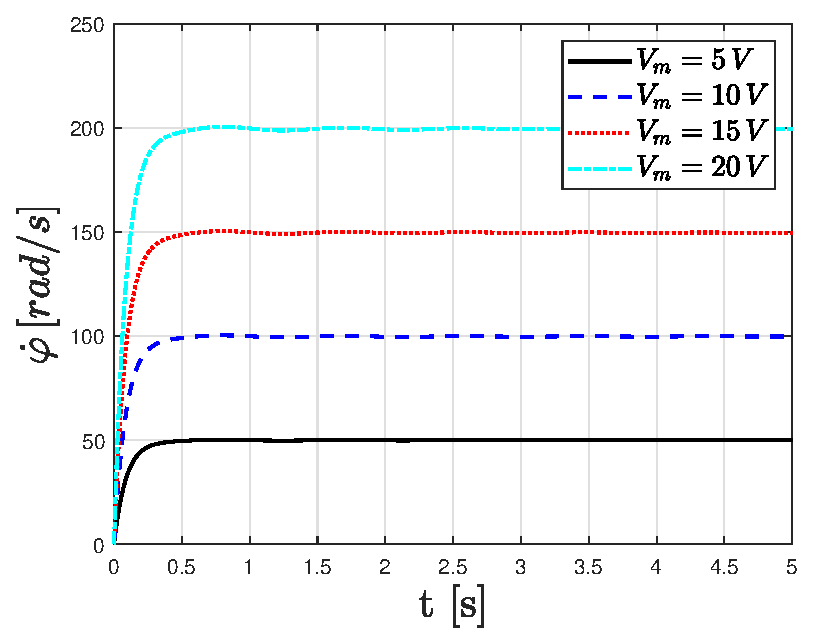
\includegraphics[width=\linewidth]{plot_data/parameter/fig/Vm_sprung/phi_punkt.eps}
        \caption{Schwungrad Geschwindikeit}
        \label{fig:Vm_sprung_phi_punkt}
    \end{subfigure}
    \begin{subfigure}[b]{0.49 \linewidth}
        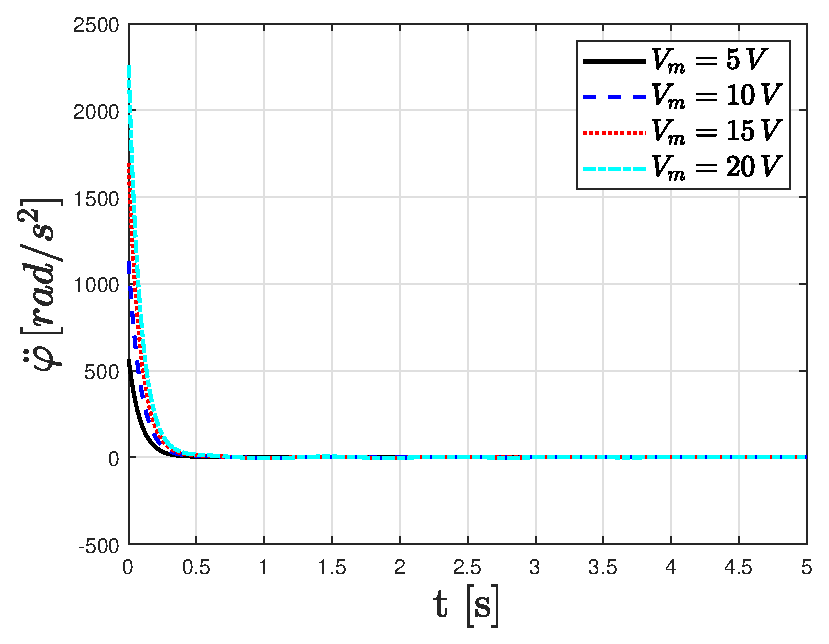
\includegraphics[width=\linewidth]{plot_data/parameter/fig/Vm_sprung/phi_punkt_punkt.eps}
        \caption{Schwungrad Beschleunigung}
        \label{fig:Vm_sprung_phi_punkt_punkt}
    \end{subfigure}
    \begin{subfigure}[b]{0.49 \linewidth}
        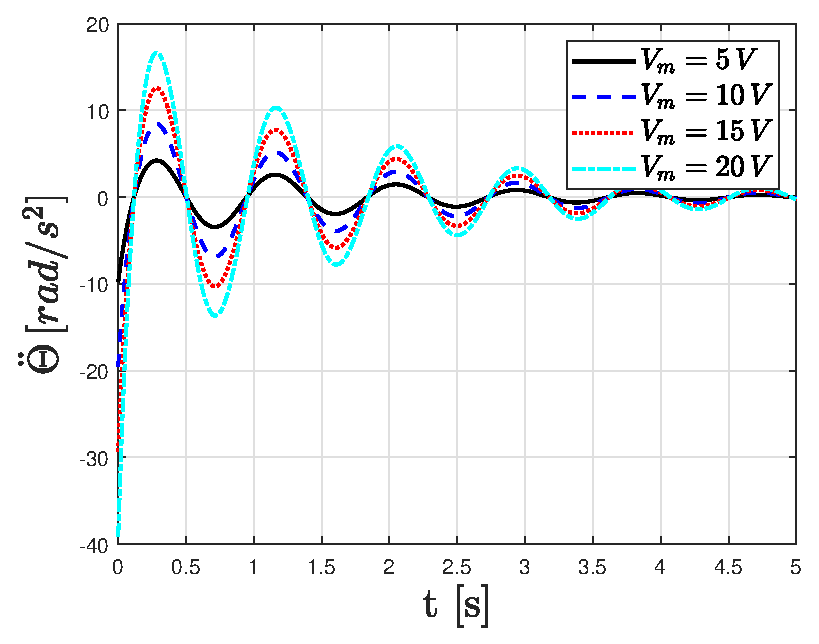
\includegraphics[width=\linewidth]{plot_data/parameter/fig/Vm_sprung/theta_punkt_punkt.eps}
        \caption{Pendel Beschleunigung}
        \label{fig:Vm_sprung_theta_punkt_punkt}
    \end{subfigure}
    \begin{subfigure}[b]{0.49\linewidth}
        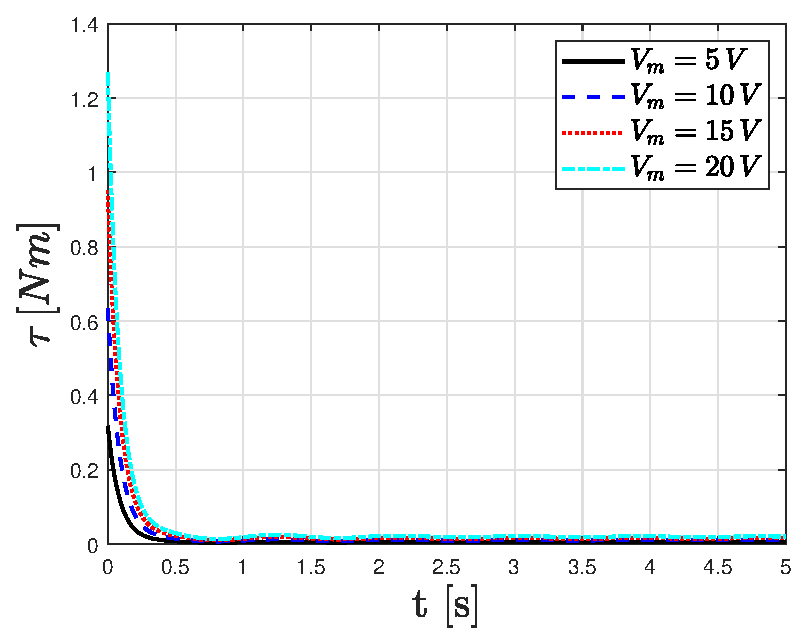
\includegraphics[width=\linewidth]{plot_data/parameter/fig/Vm_sprung/tau.eps}
        \caption{Motor Moment}
        \label{fig:Vm_sprung_tau}
    \end{subfigure}
    \begin{subfigure}[b]{0.49\linewidth}
        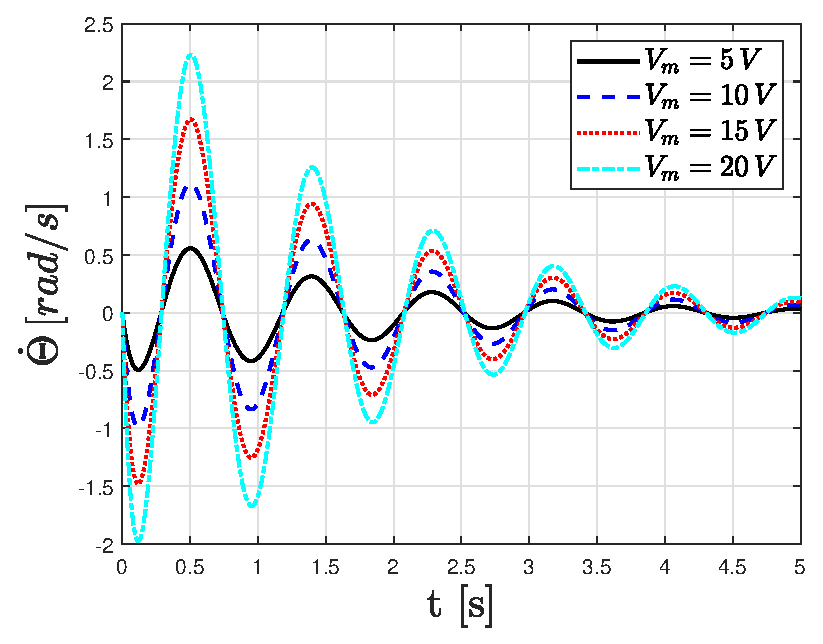
\includegraphics[width=\linewidth]{plot_data/parameter/fig/Vm_sprung/theta_punkt.eps}
        \caption{Pendel Geschwindigkeit}
        \label{fig:Vm_sprung_theta_punkt}      
    \end{subfigure}
    \begin{subfigure}[b]{0.49\linewidth}
        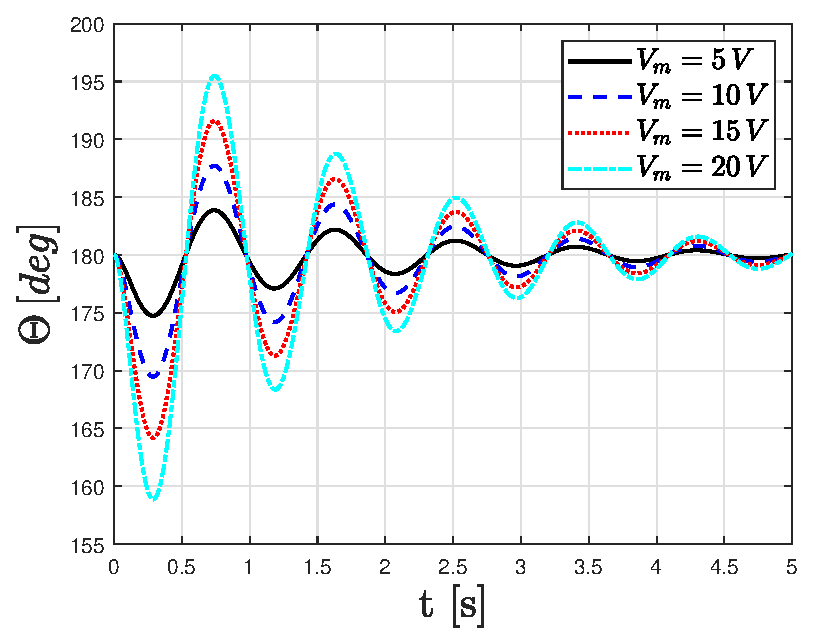
\includegraphics[width=\linewidth]{plot_data/parameter/fig/Vm_sprung/theta.eps}
        \caption{Pendel Winkel}
        \label{fig:Vm_sprung_theta}
    \end{subfigure}
        \caption{Modellantwort auf Eingangssprung der Motorspannung}
\end{wrapfigure}
In Abb.\,\ref{fig:Vm_sprung_phi_punkt} ist zu erkennen, dass der stabile Zustand der Endgeschwindigkeit des Schwungrades ungefähr zur selber Zeit ($t=\SI{0.5}{\s}$) erreicht wird.
Die dabei erreichte Endgeschwindigkeit ist direkt abhängig von der angelegten Motorsspannung $V_m$.\\
Das Maximum des Motormomentes hängt dabei ebenso von der Höhe der angelegten Motorsspannung $V_m$ ab (Abb. \ref{fig:Vm_sprung_tau}).
Das Moment erzeugt dabei eine Beschleunigung des Schwungrades (Abb. \ref{fig:Vm_sprung_phi_punkt_punkt}), die ebenso durch das Moment in Abhängigkeit zur Höhe des angelegten Motorstrommes steht.

Das Pendel wird durch das Moment in Bewegung versetzt und schwingt in Eigenfrequnz (Abb. \ref{fig:Vm_sprung_theta}). 
Die Amplitude der Pendelbewegung ist dabei abhängig von der Höhe der angelegten Motorsspannung $V_m$.

Die Pendelgeschwindigkeit (Abb. \ref{fig:Vm_sprung_theta_punkt}) hat ihren Nulldurchgang beim maximaller Amplitude des Pendelwinkels (Abb. \ref{fig:Vm_sprung_tau}), wobei die maximale Pendelgeschwindigkeit bei $\tau=\SI{180}{\degree}$ erreicht wird.

Nach erreichen der Endgeschwindigkeit des Schwungrades, geht die Beschleunigung gegen Null und das Motormomente gleicht dem Reibungsmoment (Abb. \ref{fig:Vm_sprung_tau}).
Das Pendel ist ab diesen Moment nur noch durch die Gravitation beeinfluss und schwing solange bis es in Ruheposition zurückkehrt.

\subsection*{Einfluss der Länge des Pendels zum Massezentrum des Schwungrades (l2)}
Die Länge von der Aufhängung des Pendels bis zum Masseschwerpunkt des Schwungrades ($l2$) ist ein weiterer Parameter er im Folgenden unterscuht wird.
In den Simualtionen (Abb. \ref{fig:l2}) wurde der Parameter $l2$ von $\SI{0.1}{\m}$ bis $\SI{1.5}{\m}$ variiert.
Die Motorspannung wrd dabei auf \SI{10}{\volt} gesetzt und die anderen Parameter werden ebenfals auf die Standardwerte in Tab. \ref{tab:Tabelle1.1} festgelegt.
\pagebreak

\begin{wrapfigure}{l}{.5\textwidth}
    \captionsetup[subfigure]{justification=centering,font=footnotesize}
    \begin{subfigure}[b]{0.49\linewidth}
        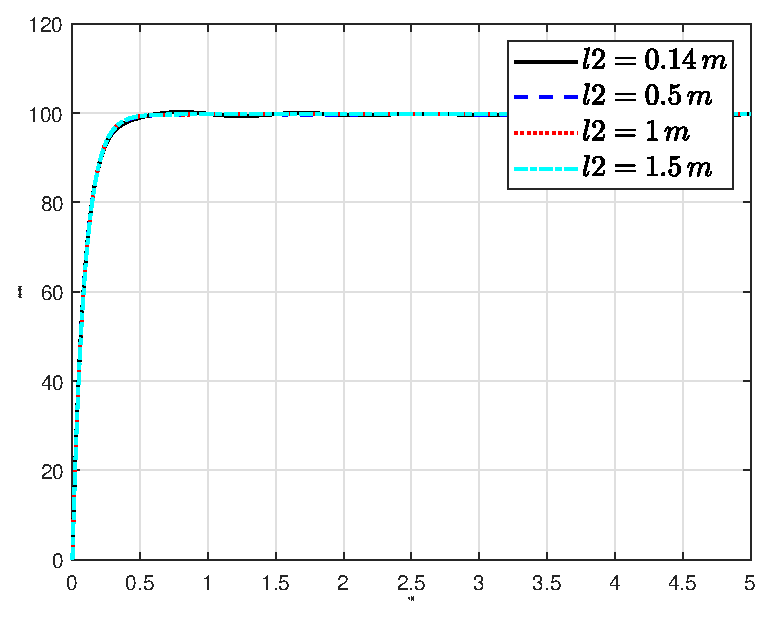
\includegraphics[width=\linewidth]{plot_data/parameter/fig/l2/phi_punkt.eps}
        \caption{Schwungrad Geschwindikeit}
        \label{fig:l2_phi_punkt}
    \end{subfigure}
    \begin{subfigure}[b]{0.49 \linewidth}
        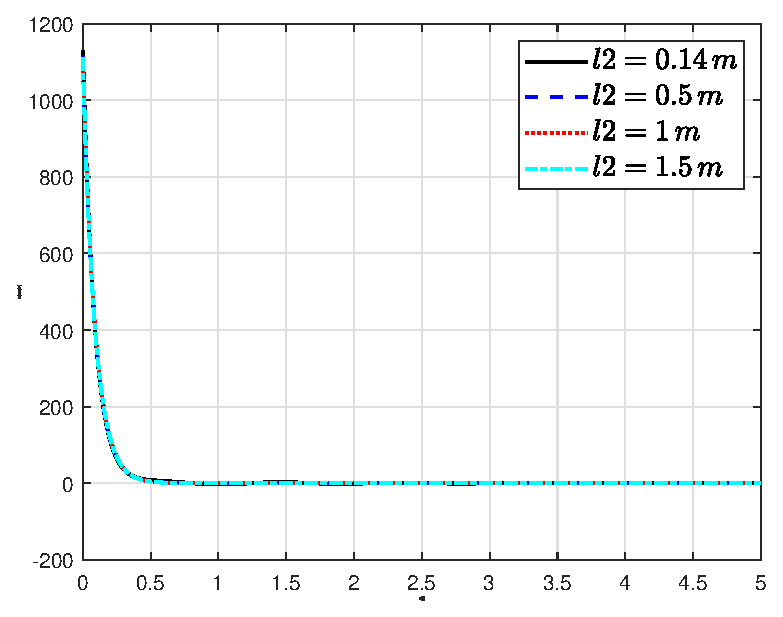
\includegraphics[width=\linewidth]{plot_data/parameter/fig/l2/phi_punkt_punkt.eps}
        \caption{Schwungrad Beschleunigung}
        \label{fig:l2_phi_punkt_punkt}
    \end{subfigure}
    \begin{subfigure}[b]{0.49 \linewidth}
        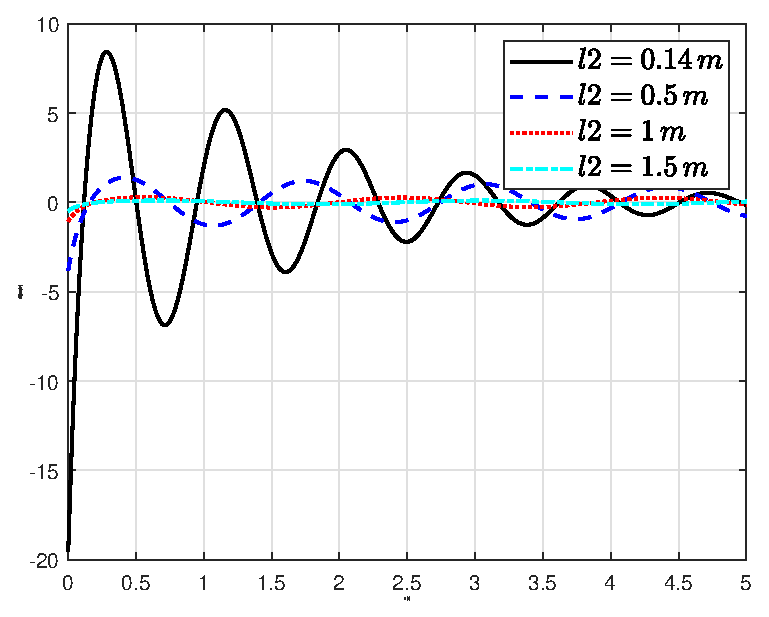
\includegraphics[width=\linewidth]{plot_data/parameter/fig/l2/theta_punkt_punkt.eps}
        \caption{Pendel Beschleunigung}
        \label{fig:l2_theta_punkt_punkt}
    \end{subfigure}
    \begin{subfigure}[b]{0.49\linewidth}
        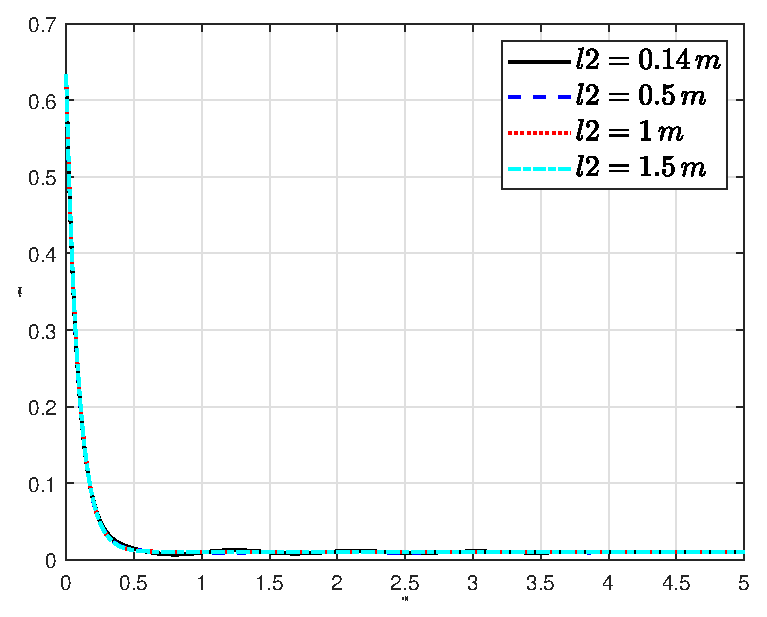
\includegraphics[width=\linewidth]{plot_data/parameter/fig/l2/tau.eps}
        \caption{Motor Moment}
        \label{fig:l2_tau}
    \end{subfigure}
    \begin{subfigure}[b]{0.49\linewidth}
        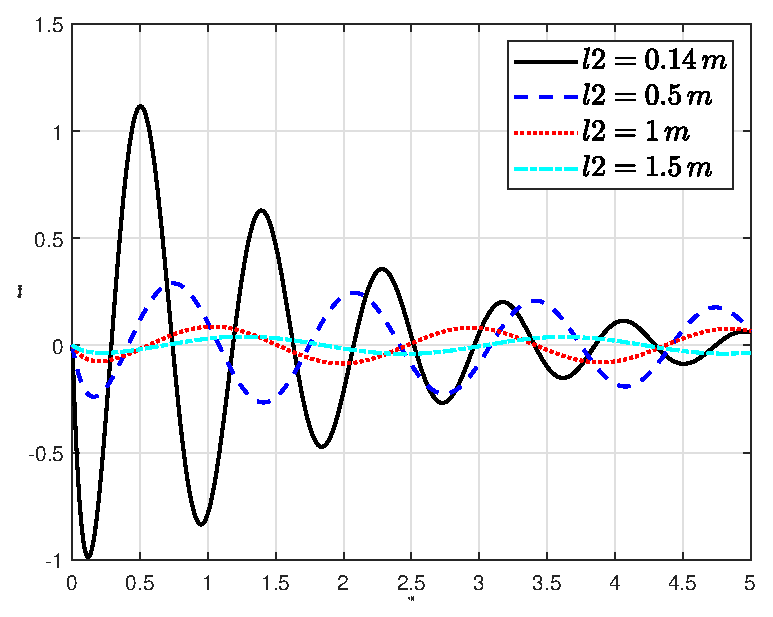
\includegraphics[width=\linewidth]{plot_data/parameter/fig/l2/theta_punkt.eps}
        \caption{Pendel Geschwindigkeit}
        \label{fig:l2_theta_punkt}      
    \end{subfigure}
    \begin{subfigure}[b]{0.49\linewidth}
        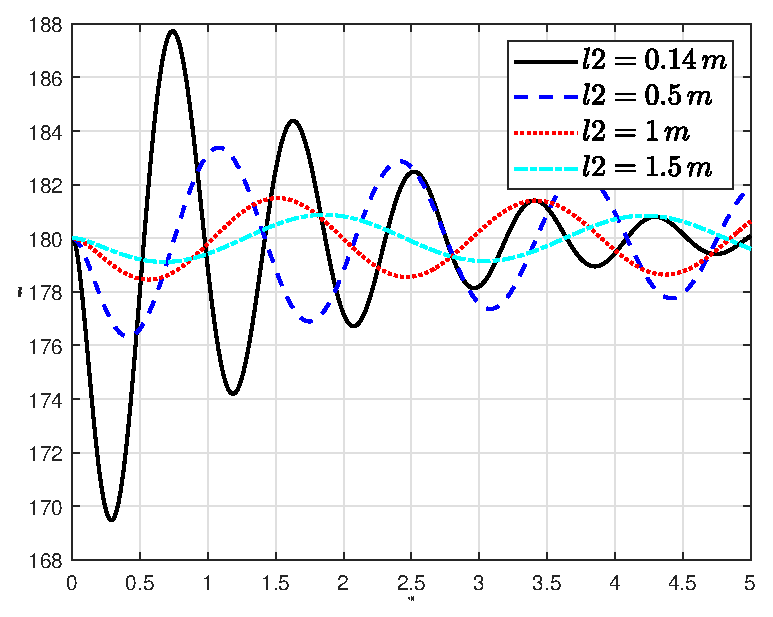
\includegraphics[width=\linewidth]{plot_data/parameter/fig/l2/theta.eps}
        \caption{Pendel Winkel}
        \label{fig:l2_theta}
    \end{subfigure}
        \caption{Modellantwort auf Varianz des Parameters: $l2$}
        \label{fig:l2}
\end{wrapfigure}
Abbildung \ref{fig:l2_phi_punkt}, \ref{fig:l2_phi_punkt}, \ref{fig:l2_tau} zeigen keine Abweichung, was zeigt das der Parameter $l2$ keinen Einfluss auf die Modellgrößen $\dot\varphi,\ddot\varphi,\tau$ hat.
Es ist jdeoch ein Einfluss auf die Parameter $\Theta,\dot\Theta,\ddot\Theta$ (Abb. \ref{fig:l2_theta}\ref{fig:l2_theta_punkt}\ref{fig:l2_theta_punkt_punkt}) zu erkennen. 

Bei kleinerer Länge $l2$ erhöht sich die Amplitude des Winkels $\Theta$ sowie dessen Geschwindigkeit $\dot\Theta$ und Beschleunigung $\ddot\Theta$. 

Ebenso ist zu erkennen das sich dei Eigenfrequenz, mit der das Pendel Schwing verändert.
Je größer die Länge $l2$ ist, desto größeres Moment musss aufgebracht werden um die gleiche Winkelauslenkung $\Theta$ zu erreichen. 
Daraus folgt, dass größere Pendelängen die Winkelantwort des Modelles verschlechtern. 

\subsection*{Einfluss des Trägheitsmoments des Schwungrads (J2)}
Der Einfluss des Trägheitsmoments des Schwungrades ($J2$), auf die Modellparameter wird in den Simulationen (Abb. \ref{fig:j2}) untersucht. 
Der Parameter $J2$ wird dabei von $\SI{0.0005}{\kg\m^2}$ bis $\SI{0.008}{\kg\m^2}$ variiert.
Die Motorspannung wrd dabei auf \SI{10}{\volt} gesetzt und die anderen Parameter werden ebenfals auf die Standardwerte in Tab. \ref{tab:Tabelle1.1} festgelegt.\\
\pagebreak

\begin{wrapfigure}{l}{0.5\textwidth}
    \captionsetup[subfigure]{justification=centering,font=footnotesize}
    \begin{subfigure}[b]{0.49\linewidth}
        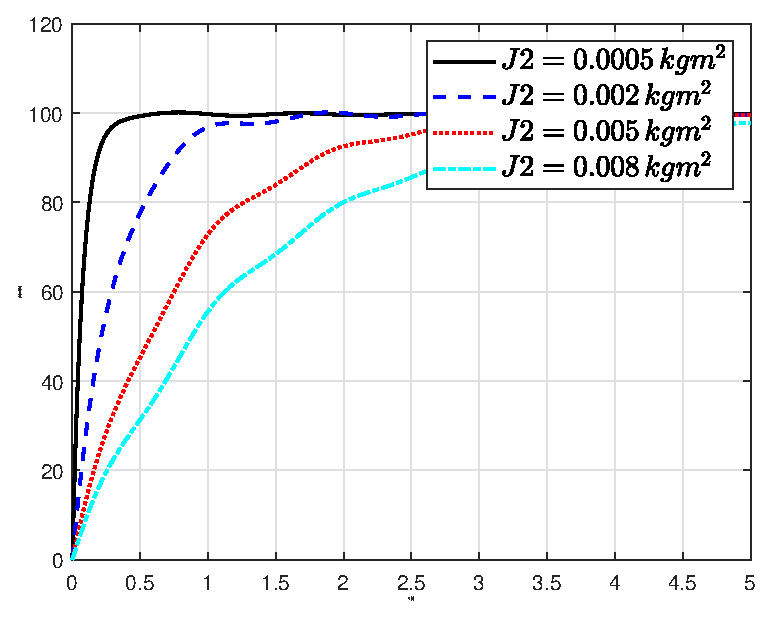
\includegraphics[width=\linewidth]{plot_data/parameter/fig/j2/phi_punkt.eps}
        \caption{Schwungrad Geschwindikeit}
        \label{fig:j2_phi_punkt}
    \end{subfigure}
    \begin{subfigure}[b]{0.49 \linewidth}
        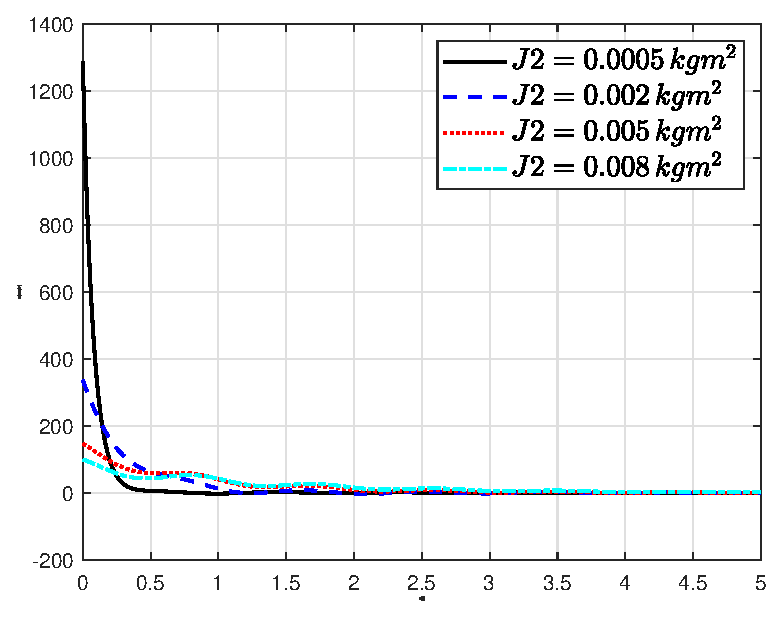
\includegraphics[width=\linewidth]{plot_data/parameter/fig/j2/phi_punkt_punkt.eps}
        \caption{Schwungrad Beschleunigung}
        \label{fig:j2_phi_punkt_punkt}
    \end{subfigure}
    \begin{subfigure}[b]{0.49 \linewidth}
        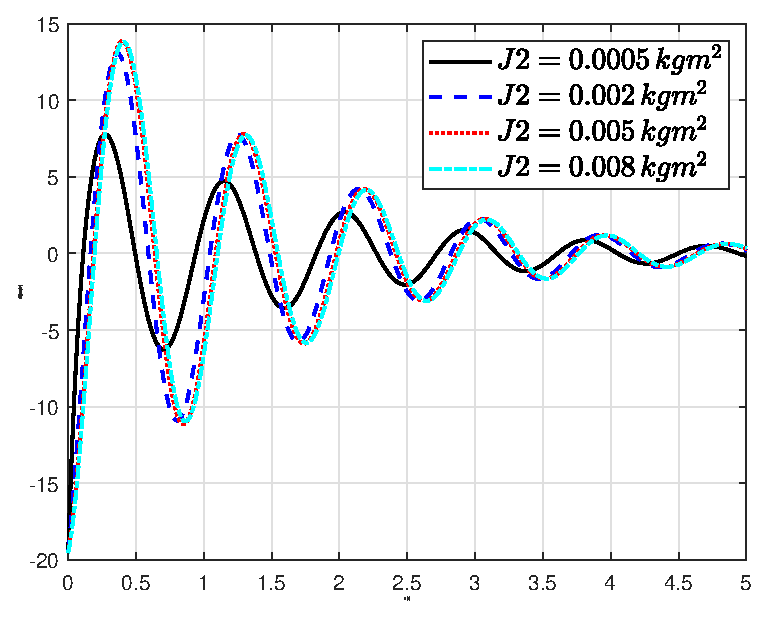
\includegraphics[width=\linewidth]{plot_data/parameter/fig/j2/theta_punkt_punkt.eps}
        \caption{Pendel Beschleunigung}
        \label{fig:j2_theta_punkt_punkt}
    \end{subfigure}
    \begin{subfigure}[b]{0.49\linewidth}
        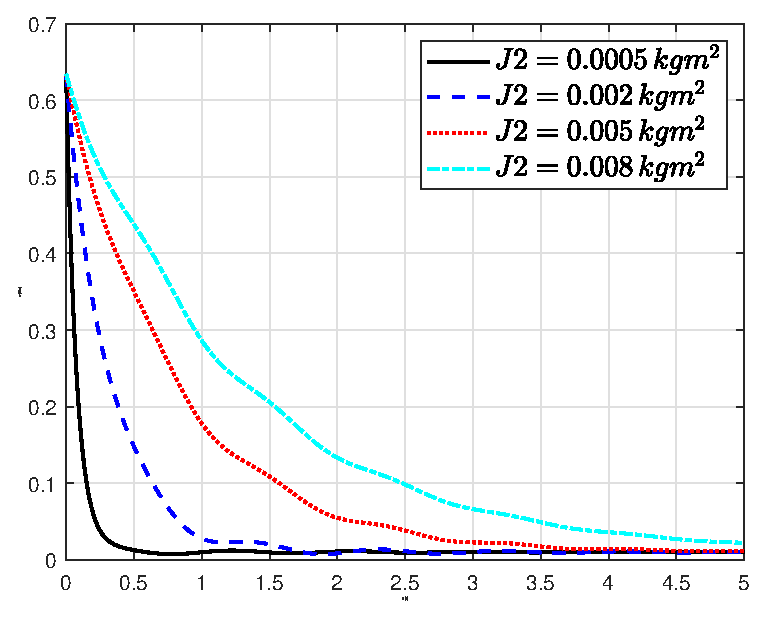
\includegraphics[width=\linewidth]{plot_data/parameter/fig/j2/tau.eps}
        \caption{Motor Moment}
        \label{fig:j2_tau}
    \end{subfigure}
    \begin{subfigure}[b]{0.49\linewidth}
        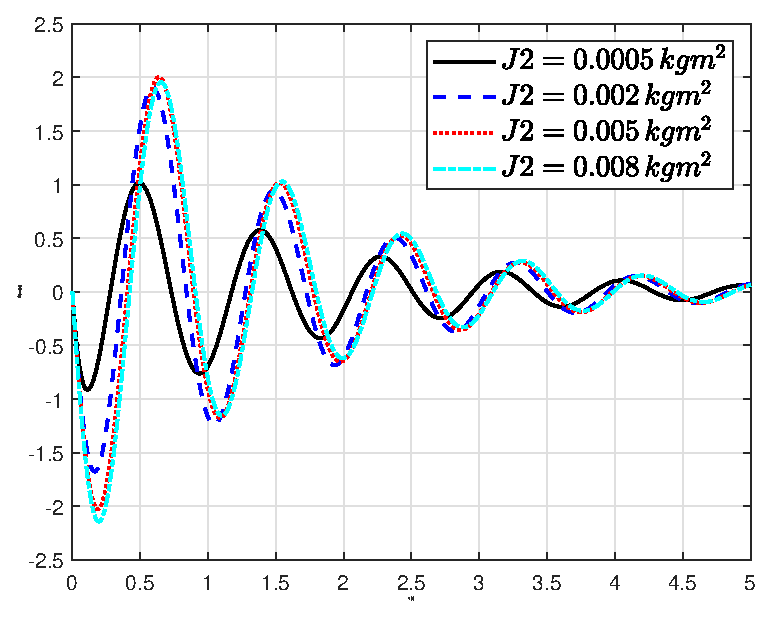
\includegraphics[width=\linewidth]{plot_data/parameter/fig/j2/theta_punkt.eps}
        \caption{Pendel Geschwindigkeit}
        \label{fig:j2_theta_punkt}      
    \end{subfigure}
    \begin{subfigure}[b]{0.49\linewidth}
        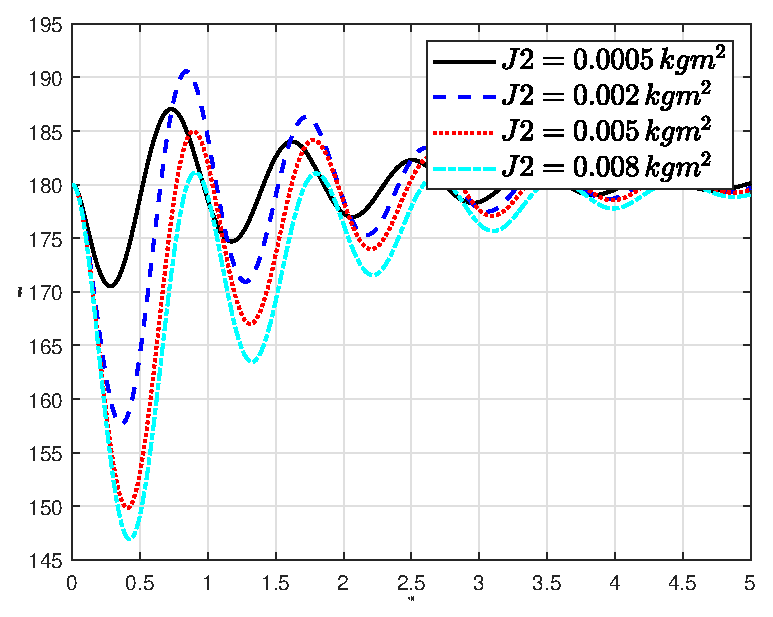
\includegraphics[width=\linewidth]{plot_data/parameter/fig/j2/theta.eps}
        \caption{Pendel Winkel}
        \label{fig:j2_theta}
    \end{subfigure}
        \caption{Modellantwort auf Varianz des Parameters: $J2$}
        \label{fig:j2}
\end{wrapfigure}
Die stationäre Endgeschwindigkeit des Schwungrades, wird durch den Parameter $J2$ stark beinflusst (Abb. \ref{fig:j2_phi_punkt}). 
Bei erhöhter Trägheit des Schwungrades erhöht sich die Anstiegszeit, bis ein eingeschwungener Zustand erreicht wird.
Der Wert konvergiert allerdings bei allen Werten von $J2$ gegen die gleiche Endgeschwindigkeit.\\

Die Beschleunigung des Schwungrades wird ebenfalls stark beinflusst (Abb. \ref{fig:j2_phi_punkt_punkt}).
Hierbei ist zu erkennen, dass ein erhöhtes Trägheitsmoment die maximale Beschleunigung bei $t\approx\SI{0}{\s}$ verringert. 
Ebenso wird der stationäre Zustand später erreicht und mit weiterer Erhöhung des Parameters ist ein Schwingen der Beschleunigung zu erkennen.\\
   
Das maximale Motormoment (Abb. \ref{fig:j2_tau}) ist bei allen Werten von $J2$ gleich, benötigt aber bei größeren Werten von $J2$ länger um den stationären Zustand zu erreichen.\\
Dadurch dass das Moment bei erhöhten Trägheitsmoment länger anliegt, wird auch eine größere Kraft auf das Pendel ausgeübt(Abb. \ref{fig:j2_theta_punkt_punkt}).\\
In Abb.\ref{fig:j2_theta} ist zu erkennen, dass ein größere Winkelauschlag des Pendels erreicht wurde.\\
Dies ist ebenso der Fall bei der Pendelbeschleunigung (Abb. \ref{fig:j2_theta_punkt_punkt}) und der Pendelgeschwindigkeit (Abb. \ref{fig:j2_theta_punkt}).\\

 Das Trägheitsmoment des Schwungrades $J2$ hat also einen positiven Einfluss auf die Winkelantwort des Modells.\\  
 
 \subsection*{Einfluss der Masse des Schwungrads (M2)}
 Der Einfluss der Masse des Schwungrades ($m2$), auf die Modellparameter wird in den Simulationen (Abb. \ref{fig:m2}) untersucht. 
 Der Parameter $J2$ wird dabei von $\SI{0.01}{\kg}$ bis $\SI{1.5}{\kg}$ variiert.
 Die Motorspannung wrd dabei auf \SI{10}{\volt} gesetzt und die anderen Parameter werden ebenfals auf die Standardwerte in Tab. \ref{tab:Tabelle1.1} festgelegt.\\
 \begin{wrapfigure}{l}{0.5\textwidth}
    \captionsetup[subfigure]{justification=centering,font=footnotesize}
    \begin{subfigure}[b]{0.49\linewidth}
        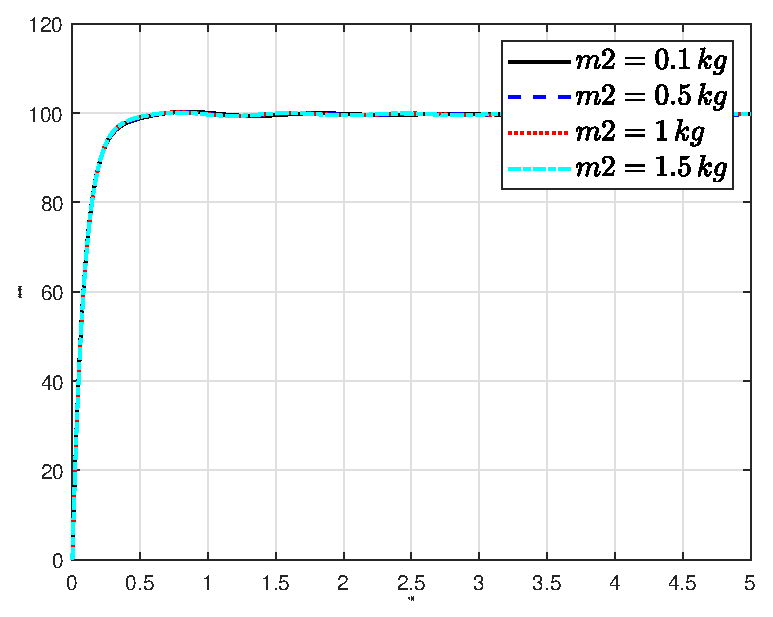
\includegraphics[width=\linewidth]{plot_data/parameter/fig/m2/phi_punkt.eps}
        \caption{Schwungrad Geschwindikeit}
        \label{fig:m2_phi_punkt}
    \end{subfigure}
    \begin{subfigure}[b]{0.49 \linewidth}
        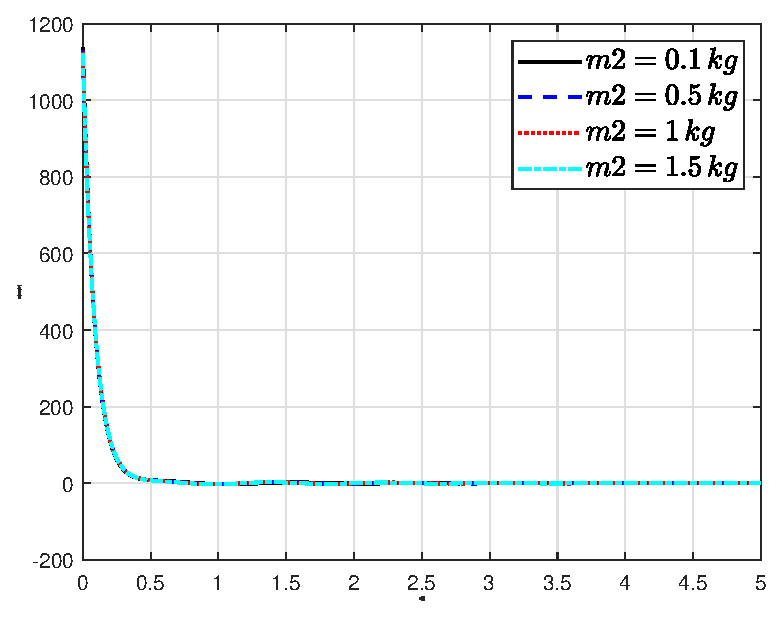
\includegraphics[width=\linewidth]{plot_data/parameter/fig/m2/phi_punkt_punkt.eps}
        \caption{Schwungrad Beschleunigung}
        \label{fig:m2_phi_punkt_punkt}
    \end{subfigure}
    \begin{subfigure}[b]{0.49 \linewidth}
        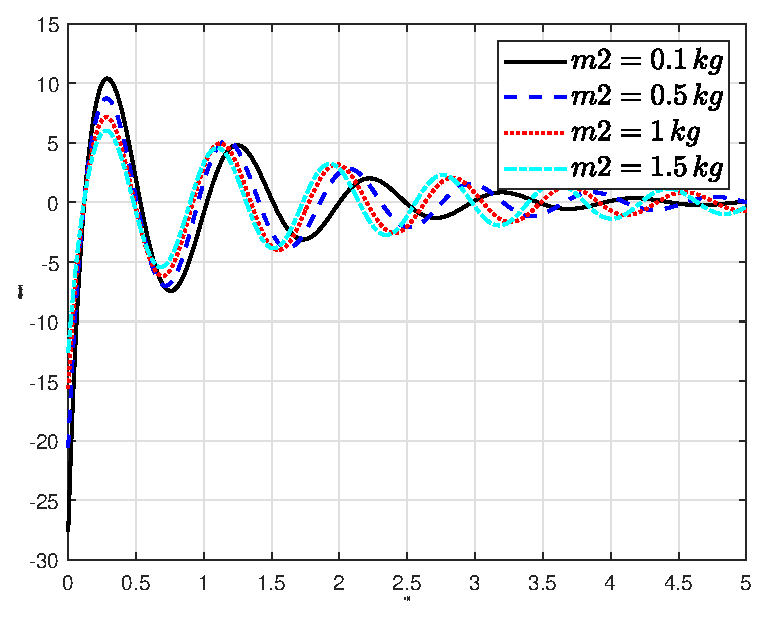
\includegraphics[width=\linewidth]{plot_data/parameter/fig/m2/theta_punkt_punkt.eps}
        \caption{Pendel Beschleunigung}
        \label{fig:m2_theta_punkt_punkt}
    \end{subfigure}
    \begin{subfigure}[b]{0.49\linewidth}
        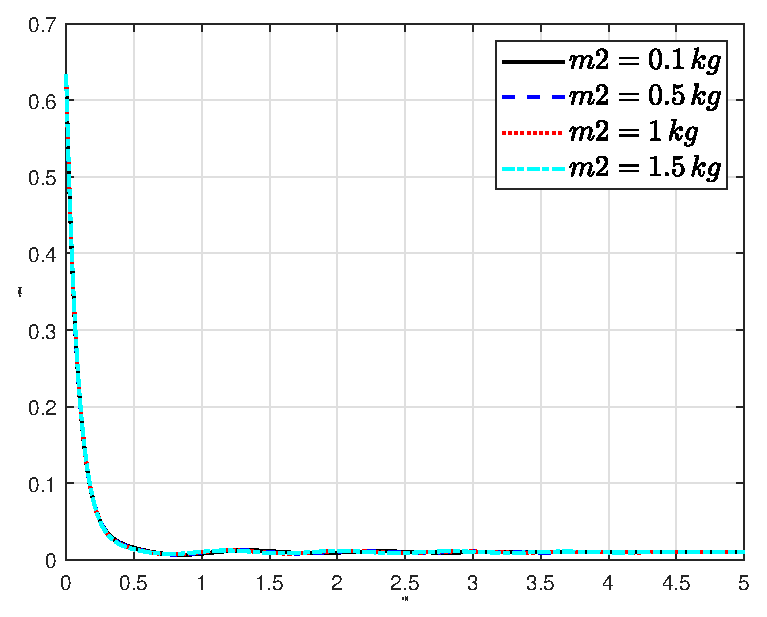
\includegraphics[width=\linewidth]{plot_data/parameter/fig/m2/tau.eps}
        \caption{Motor Moment}
        \label{fig:m2_tau}
    \end{subfigure}
    \begin{subfigure}[b]{0.49\linewidth}
        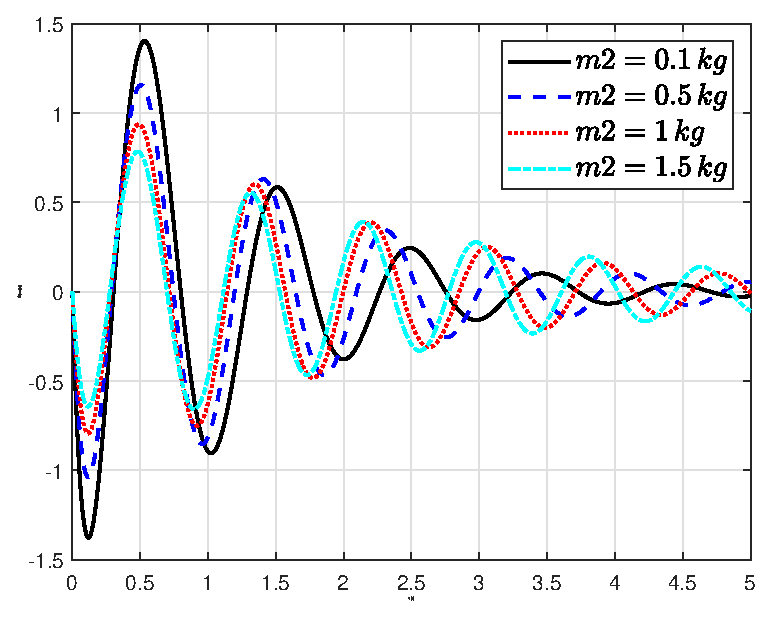
\includegraphics[width=\linewidth]{plot_data/parameter/fig/m2/theta_punkt.eps}
        \caption{Pendel Geschwindigkeit}
        \label{fig:m2_theta_punkt}      
    \end{subfigure}
    \begin{subfigure}[b]{0.49\linewidth}
        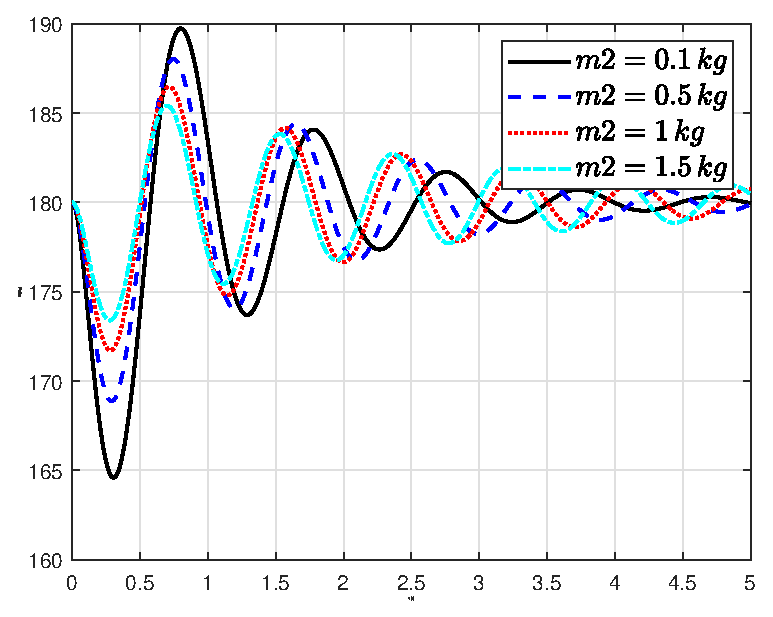
\includegraphics[width=\linewidth]{plot_data/parameter/fig/m2/theta.eps}
        \caption{Pendel Winkel}
        \label{fig:m2_theta}
    \end{subfigure}
        \caption{Modellantwort auf Varianz des Parameters: $M2$}
        \label{fig:m2}
\end{wrapfigure}

In den Simulationen ist zu erkennen das die Schwungradgeschwindigkeit (\ref{fig:m2_phi_punkt}), die Schwungradbeschleunigung (\ref{fig:m2_phi_punkt_punkt}) und das Motormoment (\ref{fig:m2_tau}) durch den Parameter $m2$ nicht beeinflusst werden.\\
Die Masse des Schwungrads hat also auf die gehalten Größen keinen Einfluss.\\

Der Winkel des Pendels (Abb. \ref{fig:m2_theta}) verrignert sich mit erhöhung der Masse $m2$. 
Dies ist auch bei der Pendelgeschwindigkeit (Abb. \ref{fig:m2_theta_punkt}) und der Pendelbeschleunigung (Abb. \ref{fig:m2_theta_punkt_punkt}) zu erkennen.\\
Dies liegt an der, durch die zusätzliche Masse, erhöhten Gewichtskraft, die auf das Pendel wirkt.\\
Ebenso wird die Dämpfung der Schwingung verändert und die Schwingungsdauer verlängert sich.\\

Die erhöhung des Parameters $m2$ trägt also zu einer Verschlechterung der Modellantwort bei.\\




\pagestyle{cyrill}
\section{Aufschwingen des Schwungrad-Pendels} \label{sec:aufschwingen}

Ziel der Aufschwungsteuerung ist, das Pendel in die obere Ruhelage zu befördern. Dazu gibt es mehrere Ansätze.
Ein 1996 bei K. J. Åström und K. Furuta \cite{SwingUp} beschriebener Ansatz ist, die Energie des Pendels zu betrachten. Im Kern werden die potentielle und kinetische Energie addiert und über einen Gain verstärkt, bis das Energieniveau dem der oberen Ruhelage des Pendels entspricht.

\begin{equation} \label{eq:Gleichung6.1}
    u = sat ( k \cdot( E + E_{\mathrm{0}} ) ) \cdot sign (\dot\theta \cdot\cos{\theta})
\end{equation}
\newline

Wobei $k$ ein Gain-Faktor ist, der bei größeren Abweichungen der Pendel-Energie effektiv durch die Ausgangsbegrenzung zu einem Zweipunkt-Regler wird, dessen Vorzeichen von dem zweiten cos-Term bestimmt wird.

\begin{figure}[H]
   \centering
   \fbox{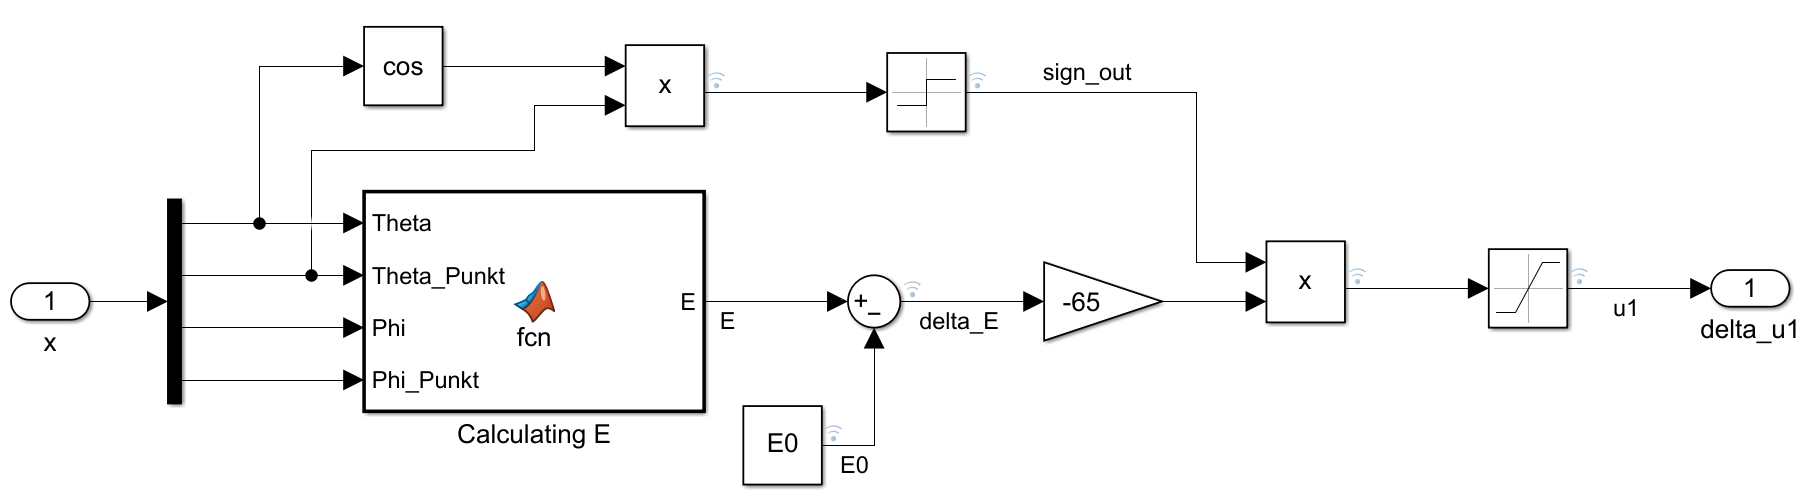
\includegraphics[width=0.95\textwidth]{Bilder/6_aufschwingen/Aufschwung-Regler_BSB.png}}
   \caption[Aufschwung-Reglerstruktur]{Aufschwung-Reglerstruktur}
   \label{fig:Bild6.1}
\end{figure}

Charmant an dieser Variante ist, dass das Energieniveau schon vor der oberen Ruhelage erreicht ist und die Energie-Zufuhr des Aktuators gestoppt wird. Die verbleibende kinetische Energie wandelt sich dann zu potentiellen Energie; während das Pendel mit dem restlichen Schwung in die obere Ruhelage läuft. Dadurch kommt das Pendel sehr ruhig in der oberen Ruhelage an und es wird ein Überschwingen vermieden.
Zur Implementierung wurden die in \autoref{sec:Modellierung} aufgestellten Energie-Gleichungen nach Lagrange genutzt – wobei die kinetische Energie des Rades in der Summe nicht berücksichtigt wird, da das den Aktuator und die Regelgröße darstellt.

\begin{equation} \label{eq:Gleichung6.2}
    E = E_{\mathrm{kin,trans}} + E_{\mathrm{pot}}
\end{equation}
\newline

Mit dieser Regelung war ein nahezu perfektes Aufschwingen möglich, bei dem der Regler nach dem Umschalten in den meisten Fällen nur noch im Bereich von ~5V gegensteuern musste, um das Pendel auf der oberen Ruheposition zu halten.

\begin{figure}[H]
   \centering
   \fbox{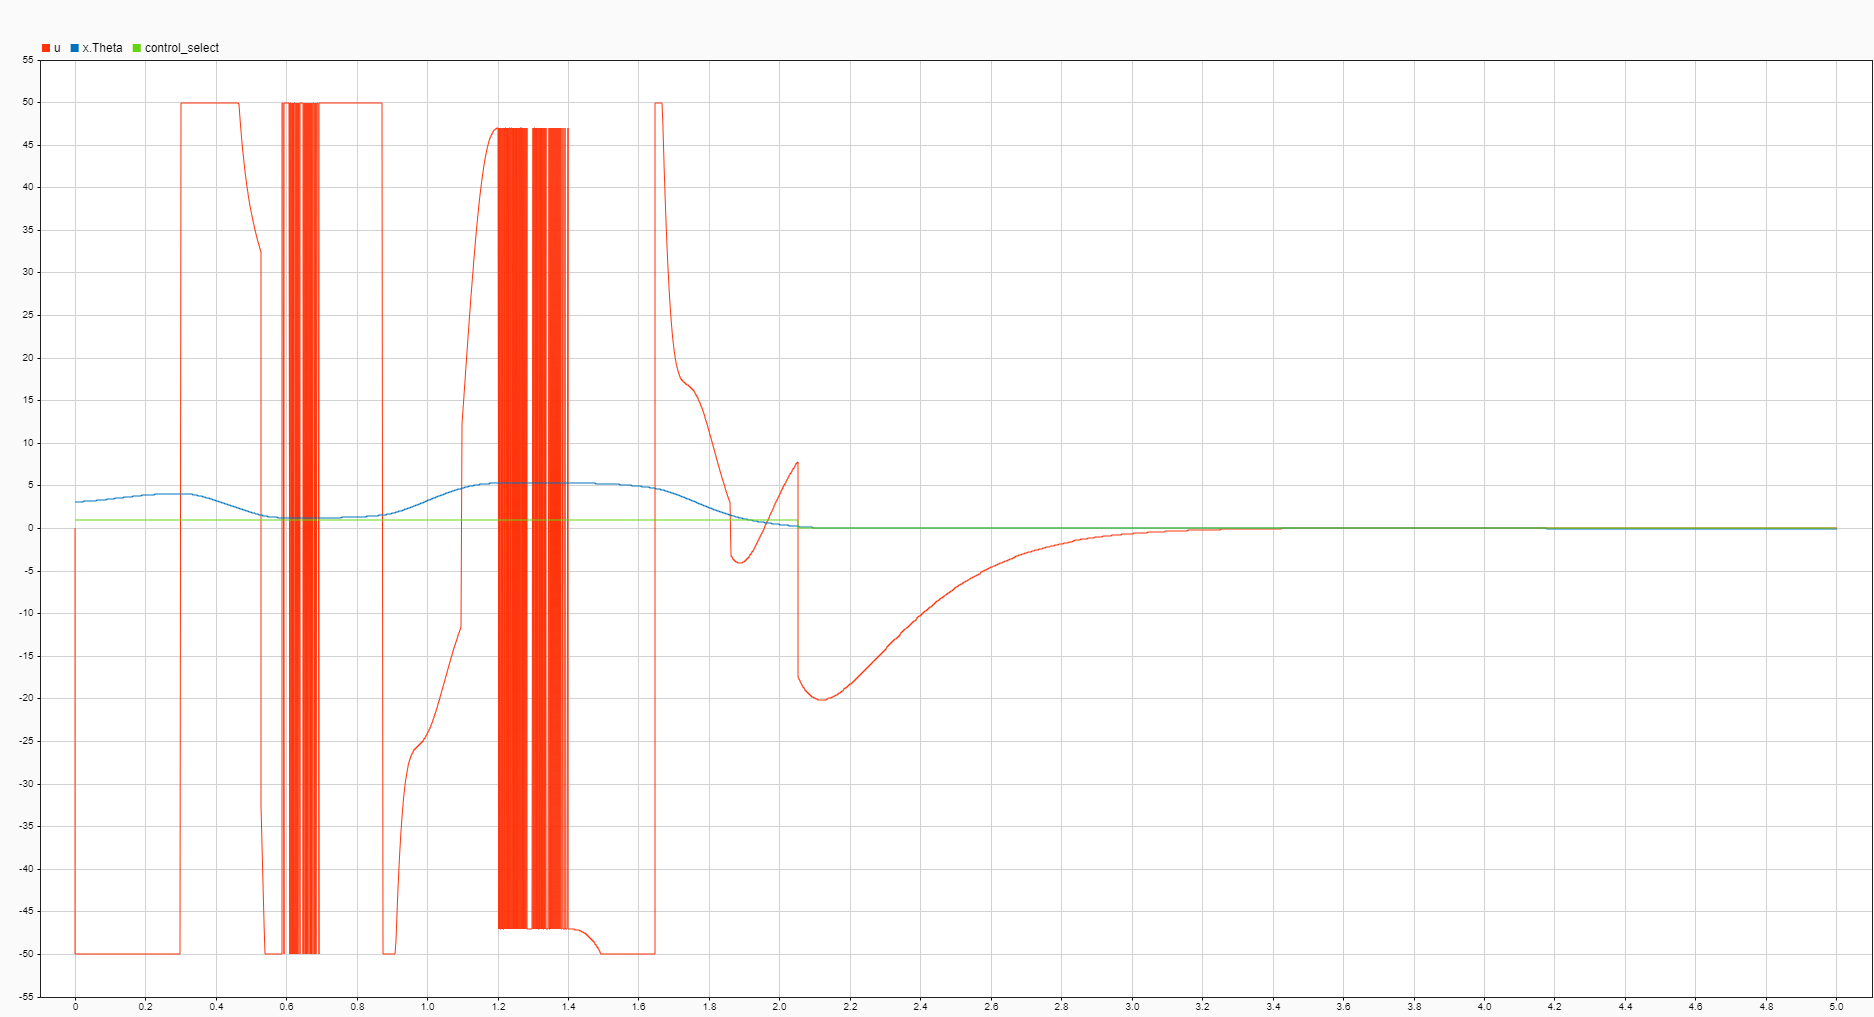
\includegraphics[width=0.95\textwidth]{Bilder/6_aufschwingen/Aufschwung-Regler.png}}
   \caption[Aufschwung-Regelung]{Aufschwung-Regelung}
   \label{fig:Bild6.2}
\end{figure}

Da in diesem Projekt aber nicht alle Zustandsvariablen gemessen werden können und stattdessen mittels einem Beobachter rekonstruiert werden sollen [vgl.: \autoref{sec:beobachter}] und dieser Beobachter nur in der Nähe des Lineariesierungs-Punktes fehlerarm arbeitet, ist die oben beschriebene Aufschwung-Regelung nicht mit dem Beobachter zu verwenden.
Daher ist in diesem Projekt ein zweiter Ansatz implementiert, welcher lediglich die aktuelle Winkelposition auswertet und wenn der aktuell gemessene Winkel kleiner als der in dem letzten Schleifen-Durchlauf ist, die Richtung des Schwungrades ändert. Schwingt das Pendel nun in einen Bereich von $\pm 14^\circ$ wird auf den Regler umgeschaltet.

\begin{figure}[H]
   \centering
   \begin{minipage}[t]{0.60\linewidth}
        \fbox{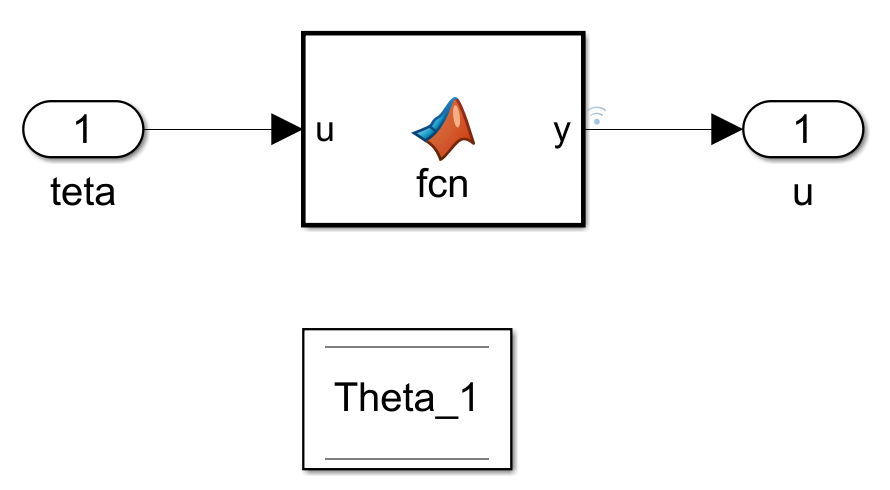
\includegraphics[width=0.95\textwidth]{Bilder/6_aufschwingen/Aufschwungsteuerung_BSB.png}}
   \end{minipage}
   \hfill
   \begin{minipage}[t]{0.3\linewidth}
        \fbox{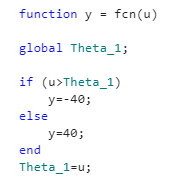
\includegraphics[width=0.95\textwidth]{Bilder/6_aufschwingen/Aufschwungsteuerung_Code.png}}
   \end{minipage}
   \caption[Aufschwung-Steuerungsstruktur]{Aufschwung-Steuerungsstruktur}
   \label{fig:Bild6.3}
\end{figure}

\begin{figure}[H]
   \centering
   \fbox{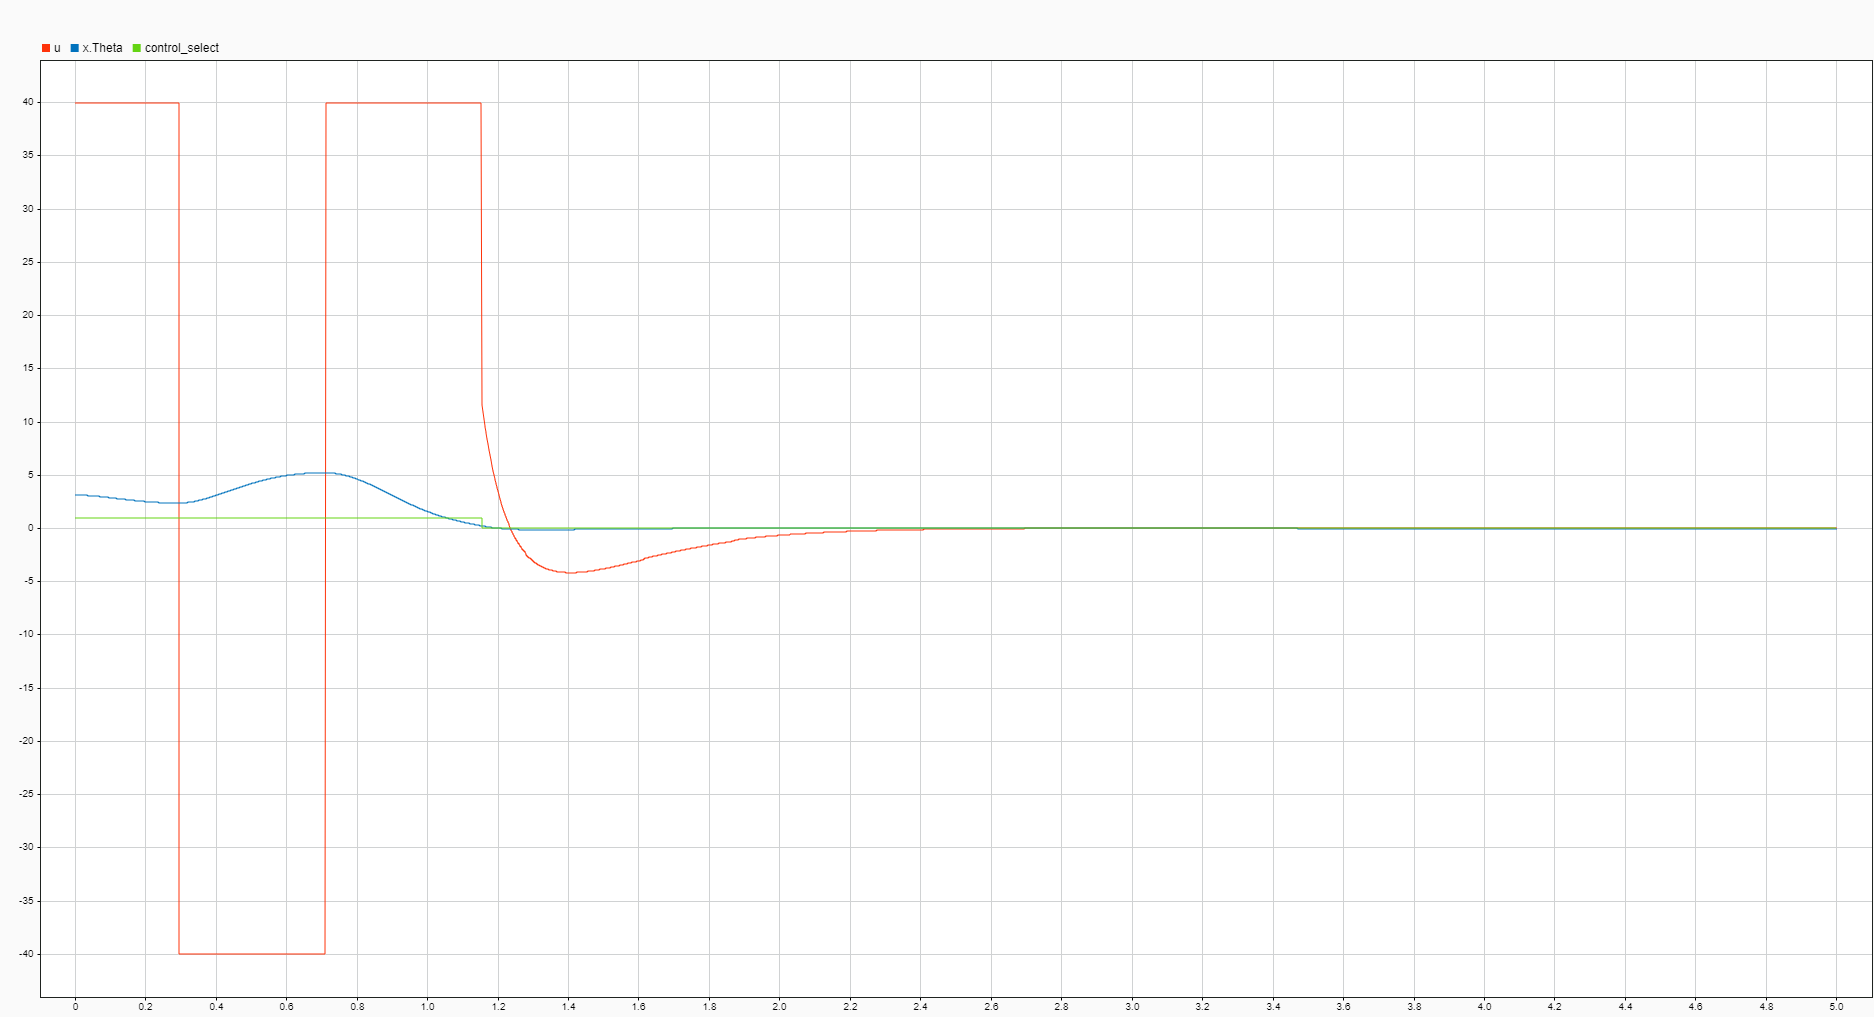
\includegraphics[width=0.95\textwidth]{Bilder/6_aufschwingen/Aufschwung-Steuerung.png}}
   \caption[Aufschwung-Steuerung]{Aufschwung-Steuerung}
   \label{fig:Bild6.4}
\end{figure}

Bei beiden Implementierungen werden die Winkel so angepasst, dass sie nur in einem Bereich von $0$ bis $2\pi$ für die Aufschwung-Steuerung respektive $-\pi$ bis $+\pi$ für den Regler liegen. Für die Aufschwung-Steuerung liegt die Unstetigkeits-Stelle in der oberen Ruhelage und für den Regler in der unteren Ruhelage. Durch die Umschaltung zwischen den beiden Regelungen erreichen die Regler niemals die Unstetigkeit während sie aktiv sind.

\begin{figure}[H]
   \centering
   \fbox{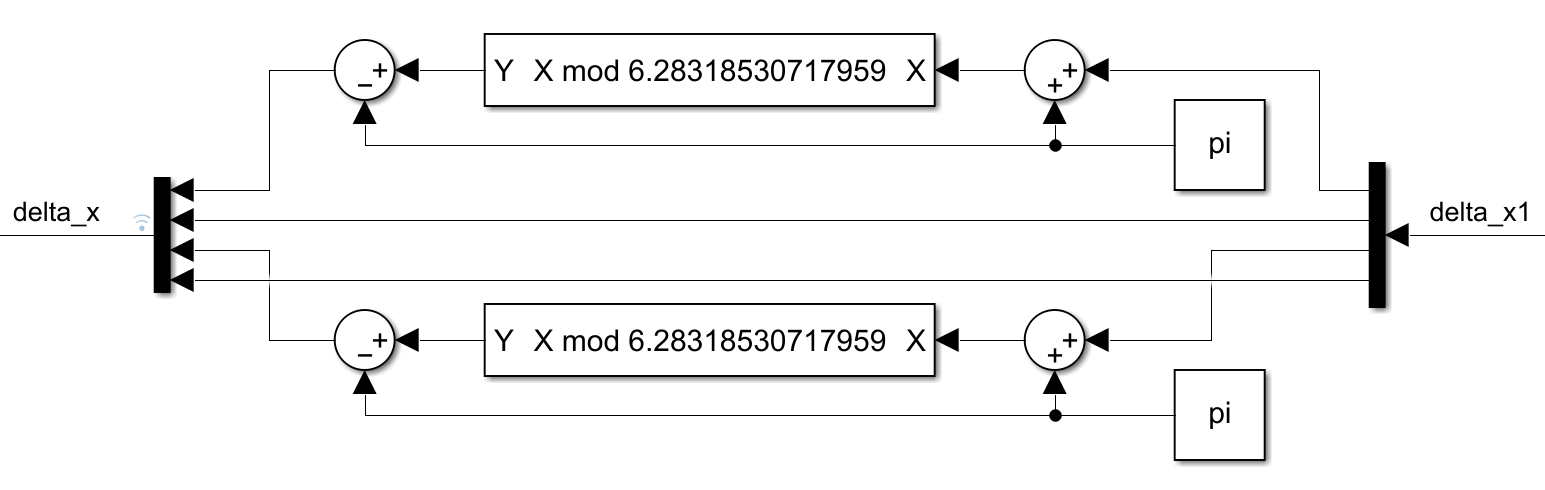
\includegraphics[width=0.95\textwidth]{Bilder/6_aufschwingen/Signal-Conditioning_for_x_BSB.png}}
   \caption[Signal-Anpassung für den Regler]{Signal-Anpassung für den Regler}
   \label{fig:Bild6.5}
\end{figure}

\begin{figure}[H]
   \centering
   \fbox{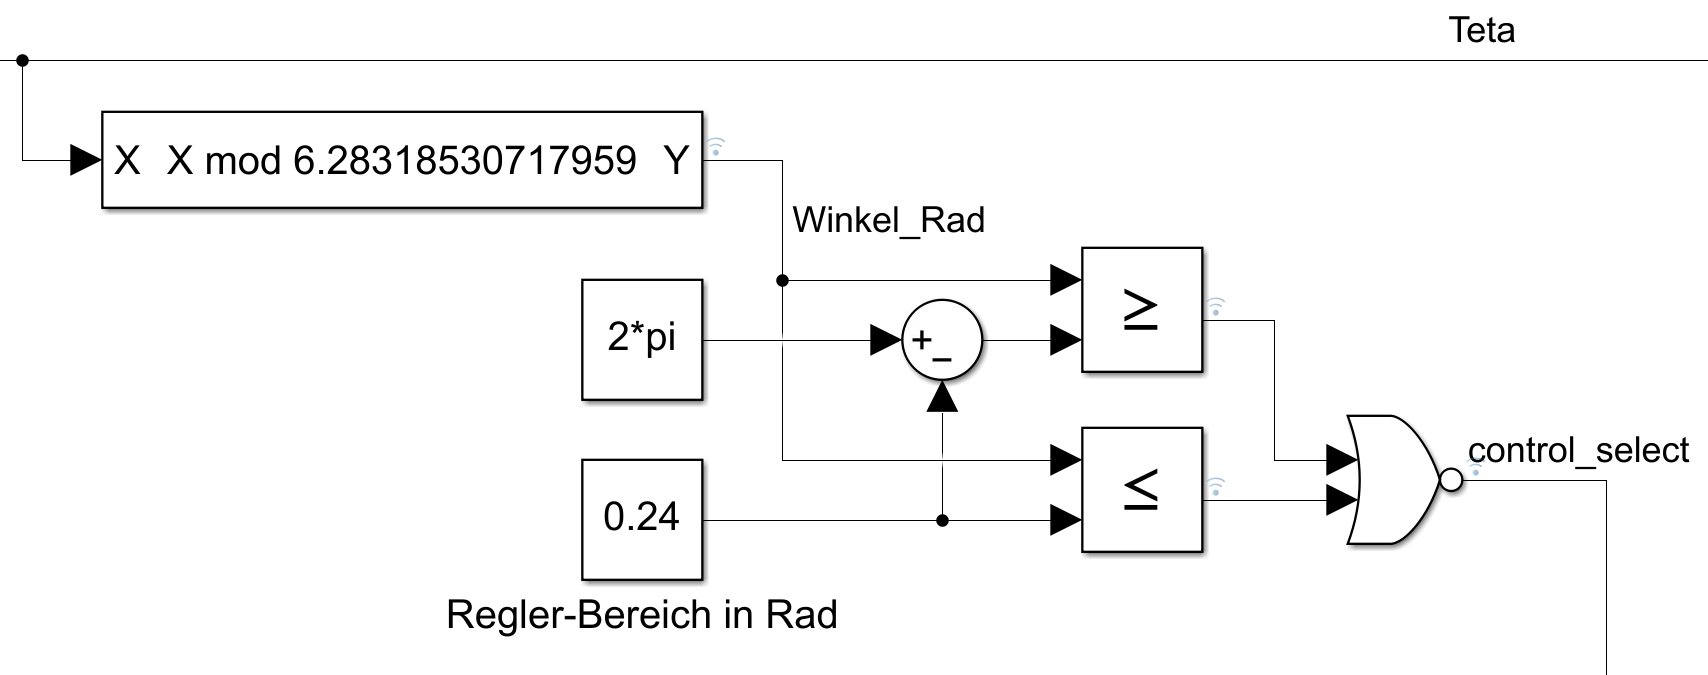
\includegraphics[width=0.95\textwidth]{Bilder/6_aufschwingen/Umschalt-Steuerung_BSB.png}}
   \caption[Umschalt-Steuerung]{Umschalt-Steuerung}
   \label{fig:Bild6.6}
\end{figure}

Es zeigte sich bei den Simulationen, dass eine maximale Motor-Spannung von 20V nicht ausreicht, um einen ausreichenden Drehmoment zu erzeugen, welcher das Pendel aufschwingen kann. Es werden bei diesem Modell mit diesem Motor mindestens 40V benötigt um das Pendel aus der unteren in die obere Ruhelage zu bewegen.

\pagestyle{sebastian}
\section{Zustandsregler} \label{sec:Zustandsregler}
Der nachfolgende Zustandsregler basiert auf einer \textbf{einfachen Zustandsrückführung}, d.h. Änderungen innerhalb des Systems werden auf die vorher definierte Ruhelage ausgeregelt.

\subsection{Reglerentwurf}
\label{sec:Reglerentwurf}

\subsubsection{Nachweis der Steuerbarkeit}
\label{sec:Nachweis der Steuerbarkeit}

Zur Implementierung einer Reglerstruktur wird vorausgesetzt, dass das System steuerbar ist. Die vollständige Steuerbarkeit ist gegeben, wenn unter Berücksichtigung der Eingangsgröße $\underline{u}(t)$ das System von jedem beliebigen Anfangszustand $\underline{x}_{\mathrm{0}}$ in jeden beliebigen Endzustand $\underline{x}_{\mathrm{e}}$ überführt werden kann. Der Nachweis erfolgt über die Auswertung der \textbf{Steuerbarkeitsmatrix} $Q_{\mathrm{s}}$. Zur Berechnung werden die Systemmatrix $A$ und die Eingangsmatrix $B$ benötigt (\autoref{eq:Gleichung7.1}).

\begin{empheq}[box=\widefbox]{align}
    \underline{Q}_{\mathrm{s}} &= \left(\underline{B}\quad\underline{A}\cdot\underline{B}\quad ... \quad\underline{A}^{(n-1)}\cdot\underline{B}\right)
    \label{eq:Gleichung7.1}
\end{empheq}
\newline
Bei \textbf{SISO}- oder \textbf{SIMO}-Systemen folgt eine quadratische Matrix, d.h. die \textbf{Bedingung} für die Steuerbarkeit lautet:

\begin{align*}
    det(\underline{Q}_{\mathrm{s}}) \neq 0.
\end{align*}
\newline
Sofern ein \textbf{MISO}- oder \textbf{MIMO}-System vorliegt, muss der \textbf{Rang} gleich $n$ bzw. $m$ sein. Die Variablen $n$ und $m$ geben die Anzahl der linear unabhängigen Zeilen und Spalten wieder. \\
Falls

\begin{align*}
    n &> m: \\
    rank(\underline{Q}_{\mathrm{s}}) &= m
\end{align*}
\newline
oder
\begin{align*}
    n &< m: \\
    rank(\underline{Q}_{\mathrm{s}}) &= n
\end{align*}
\newline
gilt, ist das System steuerbar.

\clearpage

Durch \textbf{Anwendung} der Vorschrift aus \autoref{eq:Gleichung7.1} folgt die Steuerbarkeitsmatrix des inversen Pendels in der instabilen Ruhelage zu:

\begin{align*}
    \underline{Q}_{\mathrm{s}} &= 
    \begin{bmatrix}
        0 & -1.9548 & 24.5620 & -381.4330 \\
        -1.9548 & 24.5620 & -381.4330 & 4.5979\cdot 10^{3} \\
        0 & 113.0101 & -1.2831\cdot 10^{3} & 1.4670\cdot 10^{4} \\
        113.0101 & -1.2831\cdot 10^{3} & 1.4670\cdot 10^{4} & -1.6797\cdot 10^{5}
    \end{bmatrix}.
\end{align*}
\newline
Die Matrix ist quadratisch. Die \textbf{Determinante} folgt zu:

\begin{empheq}[box=\widefbox]{align}
    det(\underline{Q}_{\mathrm{s}}) \approx 12.24\cdot 10^{7}.
    \label{eq:Gleichung7.2}
\end{empheq}
\newline
Das implementierte System ist \textbf{steuerbar}.

\subsubsection{Reglergesetz}
\label{sec:Reglergesetz}

Das allgemeine \textbf{Reglergesetz} für die Zustandsrückführung ist nachfolgend gezeigt. Die Systemstruktur kann der \autoref{fig:Bild7.1} entnommen werden. Gleichungen zur Berechnung der Matrix $K$ folgen in \autoref{sec:LMI}.

\begin{empheq}[box=\widefbox]{align}
    \underline{u}(t) &= -\underline{K}\cdot\underline{x}(t)
    \label{eq:Gleichung7.3}
\end{empheq}

\begin{figure}[H]
    \centering
    \begin{tikzpicture}[framed][domain=0:0]
        % Umgebung
        \draw[thin,color=black] (-1,0);
        % Rechteck - Strecke
        \node at (3,0) [rectangle, draw, very thick] (strecke) {\Large Strecke};
        % Pfeil \underline{y}
        \draw[-{Implies}, double, very thick] (4.03,0) -- (4.7,0);
        % \underline{y}
        \node[text width=1cm] at (4.7, 0.3) {$\underline{y}$};
        % Rechteck - \underline{K}
        \node at (1.8,-3) [rectangle, draw, very thick] (k) {\Large $-\underline{K}$};
        % Pfeil \underline{x}
        \draw[double, very thick] (3.5,-0.37) -- (3.5,-2.99);
        \draw[-{Implies}, double, very thick] (3.46,-3) -- (2.45,-3);
        % Fix der Biegung des Pfeils für \underline{x}
        \draw[very thick] (3.46,-3.032) -- (3.55,-3.032);
        \draw[very thick] (3.532,-3.03) -- (3.532,-2.98);
        % \underline{x}
        \node[text width=1cm] at (4.2, -1.6) {$\underline{x}$};
        % Pfeil \underline{u}
        \draw[double, very thick] (1.13,-3) -- (0.265,-3);
        \draw[double, very thick] (0.25,-2.95) -- (0.2,-0.013);
        \draw[-{Implies}, double, very thick] (0.25,0) -- (1.98,0);
        % Fix der Biegung des Pfeils für \underline{x}
        \draw[very thick] (0.265,-3.032) -- (0.2,-3.032);
        \draw[very thick] (0.217,-3.032) -- (0.217,-2.95);
        \draw[very thick] (0.168,-0.02) -- (0.168,0.051);
        \draw[very thick] (0.168,0.032) -- (0.27,0.032);
        % \underline{x}
        \node[text width=1cm] at (0.27, -1.6) {$\underline{u}$};
        % Rechteck - Regler (grün)
        \draw [rectangle, draw, very thick, green, dashed] (0.7,-2.4) rectangle (3,-3.6);
        \node[text width=3cm, green] at (2.8, -4) {Regler};
    \end{tikzpicture}
    \caption[Systemstruktur mit einfacher Zustandsrückführung]{Systemstruktur mit einfacher Zustandsrückführung}
    \label{fig:Bild7.1}
\end{figure}

\subsubsection{Lineare Matrixungleichungen}
\label{sec:LMI}

Die Berechnung der Reglermatrix K wird mit \textbf{quadratischen Ljapunov-Funktionen} und der \textbf{exponentiellen Stabilität} motiviert. Im ersten Schritt werden die Polstellenregionen lediglich durch die Vorgabe einer Decay-Rate $\alpha$  eingeschränkt. Die \textbf{Linearen Matrixungleichungen (LMI)} sind in \autoref{eq:Gleichung7.4} dargestellt. Zur Visualisierung der Einschränkungen dient \autoref{fig:Bild7.2}. Das Lösen der LMI's, insbesondere der \autoref{eq:Gleichung7.5} erfolgt mithilfe der Matlab-Toolbox \textbf{Robust-Control-Toolbox} (Linear Matrix Inequalities).

\begin{align}
    \begin{split}
        \underline{0} &> \underline{A}\cdot\underline{X} + \underline{X}\cdot\underline{A}^T - \underline{B}\cdot\underline{M} -\underline{M}^T\cdot\underline{B}^T + 2\cdot\alpha\cdot\underline{X}\\\\
        \underline{X} &> \underline{0}
    \end{split}
    \label{eq:Gleichung7.4}
\end{align}
\newline
mit
\begin{empheq}[box=\widefbox]{align}
    \underline{K} &= \underline{M}\cdot\underline{X}^{-1}
    \label{eq:Gleichung7.5}
\end{empheq}

\begin{figure}[H]
    \centering
    \begin{tikzpicture}[framed][domain=0:0]
        % Umgebung
        \draw[very thin,color=black] (-0.1,-1.1);
        
        % Alpha-Grenze
        \draw[dashed] (-0.8,-4) -- (-0.8,4);            
        % Alpha-Pfeil
        \draw[-stealth] (0,-2.5) -- (-0.8,-2.5) node[midway, above] {$\alpha$};
        
        % Koordinatenursprung
        \node[text width=1cm] at (0.6, -0.3) {0};

        % X-Achse
        \draw[->] (-4.2,0) -- (2,0) node[right] {$Re$}; 
        % Y-Achse
        \draw[->] (0,-4) -- (0,4) node[above] {$Im$};
        
        \begin{scope}
            % Clipping Maske zur Begrenzung
            \clip (-5,-4) rectangle (-0.8,4);
            
            % Bereich füllen
            \draw[pattern={crosshatch}, pattern color=grey, draw = white] (-4.0, -4.5) rectangle (3.2, 9);
        \end{scope}

        % Beschriftung des Polstellenbereichs
        \node[text width=3cm] at (-1.2,0.5) {$S(\alpha)$};
    \end{tikzpicture}
    \caption[Einschränkung der Polregion bei exponentieller Stabilität]{Einschränkung der Polregion bei exponentieller Stabilität zu $S(\alpha)$}
    \label{fig:Bild7.2}
\end{figure}

Sofern die Einschränkung mittels Decay-Rate nicht ausreicht, um die Voraussetzungen aus \autoref{sec:Einfuehrung} zu erreichen, werden zusätzliche LMI's eingeführt, welche weitere Einschränkungen mittels Kegel und Halbkreis vornehmen (\autoref{eq:Gleichung7.6} und \autoref{fig:Bild7.3}).

\begin{align}
    \begin{split}
        \underline{0} &> \underline{A}\underline{X} + \underline{X}\underline{A}^T - \underline{B}\underline{M} -\underline{M}^T\underline{B}^T + 2\alpha\underline{X}\\\\
        \underline{0} &>
        \begin{pmatrix}
            (\underline{A}\underline{X} + \underline{X}\underline{A}^T - \underline{B}\underline{M} - \underline{M}^T\underline{B}^T)\sin\theta & (\underline{A}\underline{X} - \underline{X}\underline{A}^T - \underline{B}\underline{M} + \underline{M}^T\underline{B}^T)\cos\theta \\\\
            (\underline{X}\underline{A}^T - \underline{A}\underline{X} + \underline{B}\underline{M} - \underline{M}^T\underline{B}^T)\cos\theta & (\underline{A}\underline{X} + \underline{X}\underline{A}^T - \underline{B}\underline{M} - \underline{M}^T\underline{B}^T)\sin\theta
        \end{pmatrix}\\\\
        \underline{0} &> 
        \begin{pmatrix}
            -r\underline{X} & \underline{A}\underline{X} - \underline{B}\underline{M} \\\\
            \underline{X}\underline{A}^T - \underline{M}^T\underline{B}^T & -r\underline{X}
        \end{pmatrix} \\\\
        \underline{X} &> \underline{0}
    \end{split}
    \label{eq:Gleichung7.6}
\end{align}

\begin{figure}[H]
    \centering
    \begin{tikzpicture}[framed][domain=0:0]
        % Umgebung
        \draw[very thin,color=black] (-0.1,-1.1);       
        % Halbkreis
        \draw[dashed] (0,-3) arc(270:90:3) -- cycle;
        
        % r-Pfeil
        \draw[-stealth] (0,0) -- (-1.24,2.74);      
        
        % r
        \node[text width=1cm] at (0, 1.6) {$r$};    
        
        % Alpha-Grenze
        \draw[dashed] (-0.8,-4) -- (-0.8,4);        
        
        % +Theta-Grenze
        \draw[dashed] (0,0) -- (-3,3);              
        
        % -Theta-Grenze
        \draw[dashed] (0,0) -- (-3,-3);                 
        % Alpha-Pfeil
        \draw[-stealth] (0,-2.5) -- (-0.8,-2.5) node[midway, above] {$\alpha$};
        
        % Koordinatenursprung
        \node[text width=1cm] at (0.6, -0.3) {0};       
        % Theta-Pfeil
        \draw[-stealth] (-0.7,0) to [bend left] (-0.5,0.5);
        
        % Theta
        \node[text width=1cm] at (-0.1, 0.2) {$\theta$};
        
        \begin{scope}
            % Clipping Maske zur Begrenzung
            \clip (-5,-4) rectangle (-0.8,4);
            
            % Bereich füllen
            \draw[pattern={crosshatch}, pattern color=grey] (0,0) -- (-2.12,2.12) arc[start angle=135, delta angle=90,radius=3] -- (0,0);
        \end{scope}
        
        % rechte Begrenzung 
        \draw[] (-0.8,-0.8) -- (-0.8,0.8);             
        
        % Beschriftung des Polstellenbereichs
        \node[text width=3cm] at (-1.2,0.5) {$S(\alpha,r,\theta)$};
        
        % X-Achse
        \draw[->] (-4.2,0) -- (2,0) node[right] {$Re$}; 
        % Y-Achse
        \draw[->] (0,-4) -- (0,4) node[above] {$Im$};
    \end{tikzpicture}
    \caption[Einschränkung der Polregion bei Erweiterung der LMI]{Einschränkung der Polregion bei Erweiterung der LMI zu $S(\alpha,r,\theta)$}
    \label{fig:Bild7.3}
\end{figure}

\subsection{Reglervalidierung am linearen Modell}
\label{sec:Reglervalidierung}

Um eine geeignete Reglerstruktur zu entwerfen, werden zuerst die \textbf{Polstellen der Systemmatrix A} bestimmt und grafisch dargestellt (\autoref{fig:Bild7.4}). Aus der Abbildung geht hervor, dass zwei der vier rein reelen Polstellen instabil sind, da diese eine Realteil größer oder gleich Null aufweisen. Dies hat ein instabiles Systemverhalten zur Folge.

\begin{align*}
    eig(\underline{A}) &=
    \begin{bmatrix}
        0 \\
        6.5169 \\
        -7.5606 \\
        -11.5214
    \end{bmatrix}
\end{align*}

\begin{figure}[H]
   \centering
   \fbox{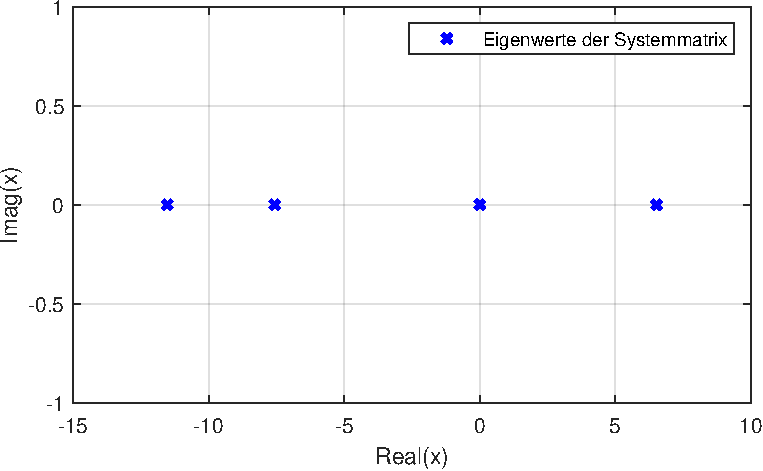
\includegraphics[width=0.8\textwidth]{Bilder/7_zustandsregler/Polstellen_der_Systemmatrix.pdf}}
   \caption[Polstellen der Systemmatrix]{Polstellen der Systemmatrix}
   \label{fig:Bild7.4}
\end{figure}

Der zu entwerfender Regler muss in der Lage sein, die maximal zulässige Eingangsspannung von $V_{\mathrm{m,Max}} = 20V$ auszureizen, jedoch nicht zu überschreiten, um größtmögliche Winkeländerungen von der definierten instabilen Ruhelage ausgleichen zu können. Die Simulationen werden mithilfe der Matlab-Erweiterung \textbf{Simulink} durchgeführt. Die Reglerstruktur ist in \autoref{fig:Bild7.5} dargestellt. Das linearisierte Zustandsraummodell verwendet gemäß Definition Delta-Größen, welche bei der Anwendung des linearen Reglers am nichtlinearen Modell berücksichtigt werden müssen. Da die entstehende K-Matrix eine Größe von (1x4) besitzt, wird fortan die Vektorschreibweise $k$ bevorzugt.

\begin{figure}[H]
   \centering
   \fbox{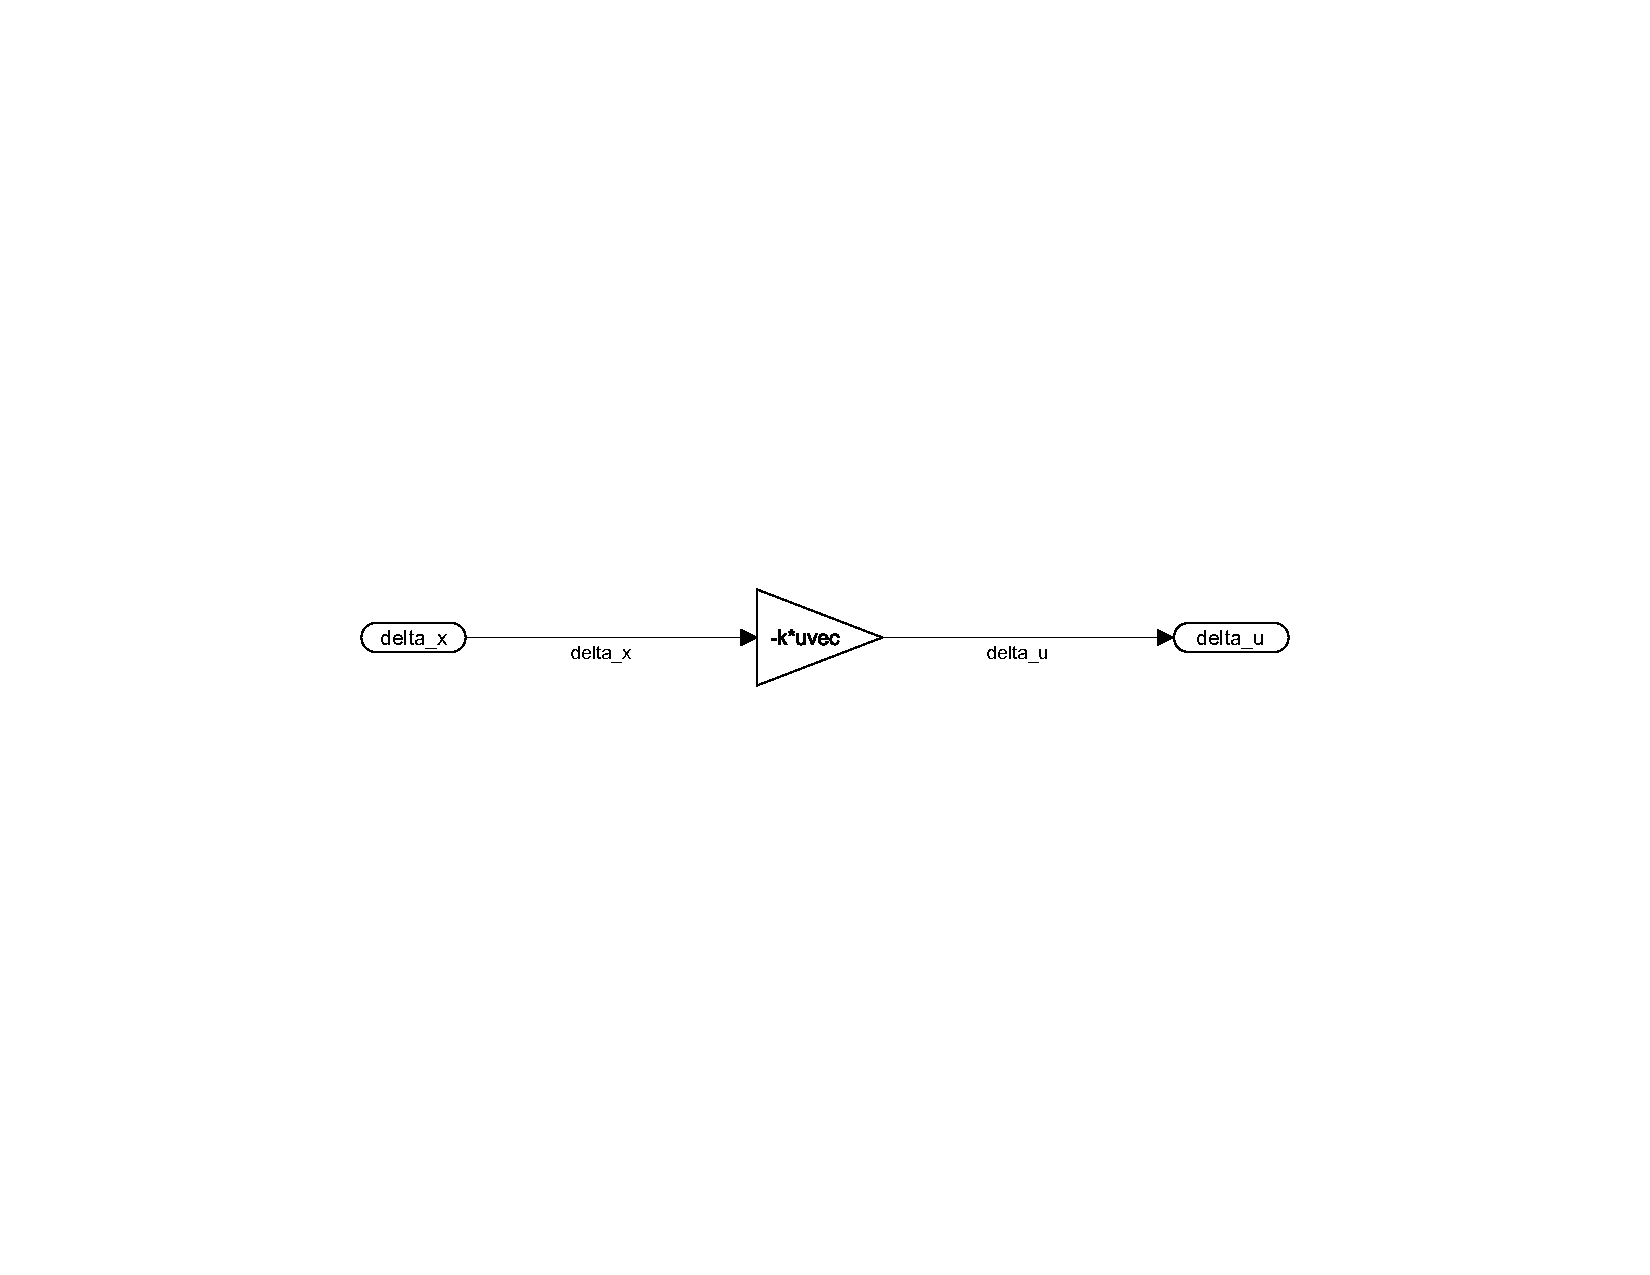
\includegraphics[width=0.95\textwidth]{Bilder/7_zustandsregler/Reglerstruktur_Simulink.pdf}}
   \caption[Simulink-Reglerstruktur]{Simulink-Reglerstruktur}
   \label{fig:Bild7.5}
\end{figure}

Im ersten Versuch wird nur die Decay-Rate $\alpha$ variiert (vgl. \autoref{fig:Bild7.2}). Der Startwinkel des Pendels wird von 15$^\circ$ solange verringert, bis der Maximalwert der anliegenden Eingangsspannung $V_{\mathrm{m}} \leq 20V$ erreicht. Zur Übersicht der Ergebnisse dient \autoref{tab:Tabelle7.1}.

\renewcommand{\arraystretch}{1.2}
\begin{table}[H]
    \centering
    \begin{tabular}{|c|c|c|c|c|c|c|}
        \hline
        & & \multicolumn{5}{c|}{ \boldmath{$\alpha$} } \\
        \makecell{\textbf{Anfangsauslenkung} \\ \textbf{Pendel [$^\circ$]}} & \textbf{Kriterium} & \textbf{1.0} & \textbf{0.5} & \textbf{0.3} & \textbf{0.1} & \textbf{0.05} \\
        \hline
        \multirow{2}{*}{15} & $V_{\mathrm{m,Max}}$ [V] & 39.107 & 31.983 & 29.184 & 26.471 & 27.351 \\
        & $V_{\mathrm{m,Max}} \leq$ 20V & - & - & - & - & -\\
        \hline
        \multirow{2}{*}{14} & $V_{\mathrm{m,Max}}$ [V] & 36.500 & 29.851 & 27.238 & 24.706 & 25.528 \\
        & $V_{\mathrm{m,Max}} \leq$ 20V & - & - & - & - & -\\
        \hline
        \multirow{2}{*}{13} & $V_{\mathrm{m,Max}}$ [V] & 33.893 & 27.719 & 25.293 & 22.941 & 23.704 \\
        & $V_{\mathrm{m,Max}} \leq$ 20V & - & - & - & - & -\\
        \hline
        \multirow{2}{*}{12} & $V_{\mathrm{m,Max}}$ [V] & 31.286 & 25.587 & 23.347 & 21.177 & 21.881 \\
        & $V_{\mathrm{m,Max}} \leq$ 20V & - & - & - & - & -\\
        \hline
        \multirow{2}{*}{11} & $V_{\mathrm{m,Max}}$ [V] & 28.679 & 23.454 & 21.401 & 19.412 & 20.057 \\
        & $V_{\mathrm{m,Max}} \leq$ 20V & - & - & - & X & -\\
        \hline
    \end{tabular}
    \caption[Auswertung von $V_{\mathrm{m}}$ für unterschiedliche Anfangsauslenkungen]{Auswertung der Eingangsspannung $V_{\mathrm{m}}$ für unterschiedliche Anfangsauslenkungen des Pendels bei Vorgabe einer Decay-Rate $\alpha$ [$\textbf{X}$ - erfüllt, $\textbf{-}$ - nicht erfüllt]} 
    \label{tab:Tabelle7.1}
\end{table}
\renewcommand{\arraystretch}{1}

Aus der Tabelle geht hervor, dass erst bei einem Anfangswinkel von 11$^\circ$ und $\alpha = 0.1$ die Spannung $V_{\mathrm{m}}$ unter 20V sinkt. Mithilfe der erweiterten LMI's wird nun versucht, ein größeren Startwinkel zu ermöglichen und weiterhin die Constraints einzuhalten. Dafür wird die Anfangsauslenkung des Pendels erneut, von 15$^\circ$ startend, verringert. Zusätzlich erfolgt eine Variation des Kegelwinkels $\Theta$ zwischen 10$^\circ$ und 60$^\circ$. Der Radius $r$ des Halbkreises variiert zwischen 11 und 15 (vgl. \autoref{fig:Bild7.3}). Die Decay-Rate $\alpha$ nimmt die bereits betrachteten Werte an. In der \autoref{tab:Tabelle7.2} und \autoref{tab:Tabelle7.3} sind die relevanten Ergebnisse dargestellt. Die vollständigen Tabellen liegen dem digitalen Anhang bei.

\begin{table}[H]
    \centering
    \begin{tabular}{|c|c|c|c|c|}
        \hline
        \boldmath{$\alpha$} & \boldmath{$\Theta [^\circ]$} & \textbf{r} & \boldmath{$V_{\mathrm{m,Max}}$} \textbf{[V]} & \makecell{\textbf{kleinste} \\ \textbf{Spannung}} \\
        \hline
        1.00 & 10 & 12 & 21.056 & -\\
        1.00 & 20 & 11 & 21.146 & -\\
        1.00 & 30 & 12 & 21.169 & -\\
        1.00 & 40 & 11 & 21.282 & -\\
        1.00 & 50 & 11 & 21.391 & -\\
        1.00 & 60 & 12 & 21.604 & -\\
        \hline
        0.50 & 10 & 13 & 20.713 & -\\
        0.50 & 20 & 13 & 20.719 & -\\
        0.50 & 30 & 13 & 20.751 & -\\
        0.50 & 40 & 13 & 20.947 & -\\
        0.50 & 50 & 13 & 20.986 & -\\
        0.50 & 60 & 12 & 21.265 & -\\
        \hline
        0.30 & 10 & 14 & 20.519 & -\\
        0.30 & 20 & 13 & 20.590 & -\\
        0.30 & 30 & 13 & 20.620 & -\\
        0.30 & 40 & 13 & 20.722 & -\\
        0.30 & 50 & 13 & 20.926 & -\\
        0.30 & 60 & 15 & 21.083 & -\\
        \hline
        0.10 & 10 & 15 & 20.294 & -\\
        0.10 & 20 & 14 & 20.398 & -\\
        0.10 & 30 & 14 & 20.442 & -\\
        0.10 & 40 & 14 & 20.598 & -\\
        0.10 & 50 & 13 & 20.777 & -\\
        0.10 & 60 & 14 & 20.972 & -\\
        \hline
        0.05 & 10 & 15 & 20.256 & X\\
        0.05 & 20 & 14 & 20.377 & -\\
        0.05 & 30 & 14 & 20.420 & -\\
        0.05 & 40 & 14 & 20.537 & -\\
        0.05 & 50 & 13 & 20.819 & -\\
        0.05 & 60 & 14 & 20.945 & -\\
        \hline
    \end{tabular}
    \caption[Auswertung von $V_{\mathrm{m}}$ bei einem Anfangswinkel von 15${^\circ}$]{Auswertung der Eingangsspannung $V_{\mathrm{m}}$ für den \textbf{Anfangswinkel 15${^\circ}$} des Pendels bei Vorgabe einer Decay-Rate $\alpha$, Kegelwinkel $\Theta$ und Radius $r$ [$\textbf{X}$ - erfüllt, $\textbf{-}$ - nicht erfüllt]}
    \label{tab:Tabelle7.2}
\end{table}

\begin{table}[H]
    \centering
    \begin{tabular}{|c|c|c|c|c|}
        \hline
        \boldmath{$\alpha$} & \boldmath{$\Theta [^\circ]$} & \textbf{r} & \boldmath{$V_{\mathrm{m,Max}}$} \textbf{[V]} & \makecell{\textbf{größte} \\ \textbf{Spannung}} \\
        \hline
        1.00 & 10 & 13 & 19.912 & -\\
        1.00 & 20 & 13 & 19.966 & -\\
        1.00 & 30 & 11 & 19.771 & -\\
        1.00 & 40 & 12 & 19.886 & -\\
        1.00 & 50 & 11 & 19.965 & -\\
        1.00 & 60 & 12 & 20.164 & -\\
        \hline
        0.50 & 10 & 12 & 19.498 & -\\
        0.50 & 20 & 11 & 19.685 & -\\
        0.50 & 30 & 11 & 19.786 & -\\
        0.50 & 40 & 11 & 19.880 & -\\
        0.50 & 50 & 14 & 19.997 & X\\
        0.50 & 60 & 13 & 19.926 & -\\
        \hline
        0.30 & 10 & 12 & 19.824 & -\\
        0.30 & 20 & 11 & 19.953 & -\\
        0.30 & 30 & 15 & 19.954 & -\\
        0.30 & 40 & 15 & 19.672 & -\\
        0.30 & 50 & 11 & 19.990 & -\\
        0.30 & 60 & 12 & 19.832 & -\\
        \hline
        0.10 & 10 & 13 & 19.326 & -\\
        0.10 & 20 & 12 & 19.489 & -\\
        0.10 & 30 & 12 & 19.436 & -\\
        0.10 & 40 & 12 & 19.621 & -\\
        0.10 & 50 & 11 & 19.904 & -\\
        0.10 & 60 & 15 & 19.803 & -\\
        \hline
        0.05 & 10 & 13 & 19.244 & -\\
        0.05 & 20 & 12 & 19.528 & -\\
        0.05 & 30 & 12 & 19.528 & -\\
        0.05 & 40 & 12 & 19.636 & -\\
        0.05 & 50 & 15 & 19.752 & -\\
        0.05 & 60 & 15 & 19.793 & -\\
        \hline
    \end{tabular}
    \caption[Auswertung von $V_{\mathrm{m}}$ bei einem Anfangswinkel von 14${^\circ}$]{Auswertung der Eingangsspannung $V_{\mathrm{m}}$ für den \textbf{Anfangswinkel 14${^\circ}$} des Pendels bei Vorgabe einer Decay-Rate $\alpha$, Kegelwinkel $\Theta$ und Radius $r$ [$\textbf{X}$ - erfüllt, $\textbf{-}$ - nicht erfüllt]}
    \label{tab:Tabelle7.3}
\end{table}

Bei einem Anfangswinkel von 15$^\circ$ wird die Eingangsspannung nicht kleiner als 20V (\autoref{tab:Tabelle7.2}). Eine Verringerung auf 14$^\circ$ führt zu einem akzeptablen Ergebnis (\autoref{tab:Tabelle7.3}). Die maximale Spannung beträgt $V_{\mathrm{m,Max}} \approx 19.997V$. Die eingestellten Parameter folgen zu:
\begin{empheq}[box=\widefbox]{align}
    \alpha = 0.50; \quad \Theta = 50^\circ; \quad r = 14.
    \label{eq:Gleichung7.7}
\end{empheq}
\newline
Bei den gewählten Parametern und der Berücksichtigung bei der Berechnung der LMI's resultieren die Werte des k-Vektors.
\begin{empheq}[box=\widefbox]{align}
    \underline{k} &= 
    \begin{bmatrix}
        -75.7055 & -9.6779 & -0.0154 & -0.1327
    \end{bmatrix}
    \label{eq:Gleichung7.8}
\end{empheq}
\newline
Die Polstellen des geschlossenen Regelkreises sind nachfolgend aufgelistet und im Vergleich zu den Polstellen der Systemmatrix in \autoref{fig:Bild7.6} dargestellt.

\begin{align*}
    eig(\underline{A}-\underline{b}\cdot\underline{k}) &=
    \begin{bmatrix}
        -6.3199 + j0.3236 \\
        -6.3199 - j0.3236 \\
        -3.1548 + j0.0000 \\
        -0.6905 + j0.0000 \\
    \end{bmatrix}
\end{align*}

\begin{figure}[H]
   \centering
   \fbox{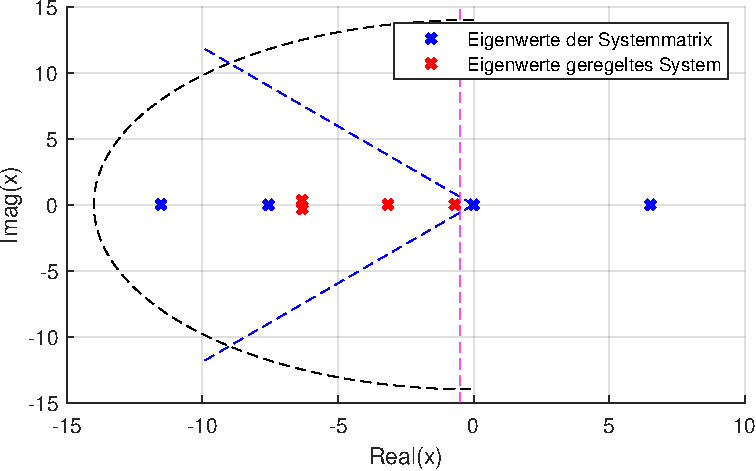
\includegraphics[width=0.8\textwidth]{Bilder/7_zustandsregler/Vergleich_der_Polstellenlagen.pdf}}
   \caption[Polstellenlagen der Systemmatrix und des geschlossenen Regelkreises]{Vergleich der Polstellenlagen der Systemmatrix A und des geschlossenen Regelkreises}
   \label{fig:Bild7.6}
\end{figure}

Der geschlossene Regelkreis weist nur Polstellen mit einem Realteil kleiner Null auf. Folglich ist das System stabil. In \autoref{fig:Bild7.7} sind der Kurvenverlauf des Pendelwinkels $\Theta$, als auch der des Schwungradwinkels $\varphi$ dargestellt. Aus den Kurvenverläufen wird geschlussfolgert, dass die implementierte Reglerstruktur das Pendel in die instabile Ruhelage zurückregelt. Die maximale Eingangsspannung von 20V wird dabei nicht überschritten. Die eingangs gesetzten Regelziele gelten als erfüllt.

\begin{figure}[H]
   \centering
   \fbox{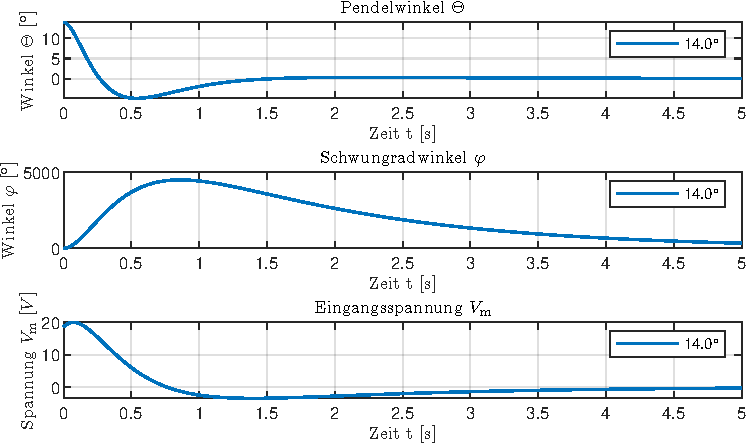
\includegraphics[width=0.95\textwidth]{Bilder/7_zustandsregler/Validierung_des_Reglers.pdf}}
   \caption[Relevante Kurvenverläufe zur Validierung des Reglers]{Relevante Kurvenverläufe zur Validierung des Reglers}
   \label{fig:Bild7.7}
\end{figure}

\subsection{Regleranwendung am nichtlinearen Modell}
\label{sec:Regleranwendung}

Bei der Anwendung des linearen Reglers am nichtlinearen Modell werden die erweiterten LMI-Parameter aus \autoref{eq:Gleichung7.7} angesetzt, d.h. der k-Vektor aus \autoref{eq:Gleichung7.8} gilt. Die relevanten Kurvenverläufe sind in \autoref{fig:Bild7.8} dargestellt. Diese ähneln den Kurvenverläufen aus \autoref{fig:Bild7.7}. Die maximale Eingangsspannung des nichtlinearen Modells ist: $V_{\mathrm{m,Max}} \approx 19.924V$. Die vorgegebenen Constrains sind eingehalten. Der lineare Regler ist in der Lage, das instabile nichtlineare System für Auslenkungen bis 14$^\circ$ zu stabilisieren.

\begin{figure}[H]
   \centering
   \fbox{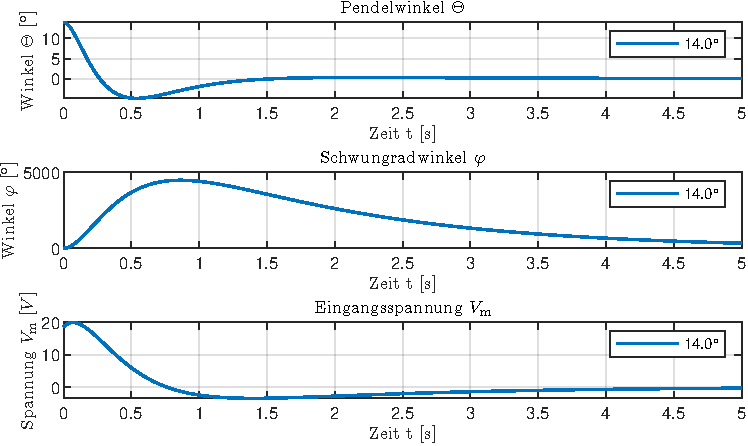
\includegraphics[width=0.95\textwidth]{Bilder/7_zustandsregler/Anwendung_des_Reglers.pdf}}
   \caption[Relevante Kurvenverläufe zur Anwendung des Reglers]{Relevante Kurvenverläufe zur Anwendung des Reglers}
   \label{fig:Bild7.8}
\end{figure}
\pagestyle{cyrill}
\section{Beobachterentwurf} \label{sec:beobachter}
\pagestyle{milan}
\section{Fazit und Ausblick} \label{sec:ausblick}
Im Umfang dieser Arbeit wurde ein mathematisches Modell des Schwungradpendels, sowie der ihn treibende DC Motor, und dessen Parameter aufgestellt (\ref{sec:Modellierung}). 
Dabei wurde ein Lagrange Ansatz gewählt und eine Bewegungsgleichung hergeleitet. 
Die so entstandene Differenzialgleichung wurde anschließend in den Zustandsraum überführt (\ref{sec:Zustandsraumdarstellung}).\\

Durch eine anschließende Linearisierung des Zustandsraummodells und dessen Verifizierung (\ref{sec:Vergleich}), konnte eine gute Steuerbarkeit und Simulierbarkeit erreicht werden.\\

Die nachfolgende Sensitivitätsanalyse bestimmte die wichtigsten Parameter und deren Einfluss auf die Modellantwort. 
Dadurch konnten Erkenntnisse hinschlicht möglicher Optimierungen, sowie dem allgemeinen Verhalten des Systems gewonnen werden (\ref{sec:sesitivitaetsanalyse}).\\

Anschließend wurden eine Methode zum Aufschwingen des Pendels erarbeitet und mithilfe von Simulationen bestätigt (\ref{sec:aufschwingen}).

Der nachfolgend entwickelte Zustandsregler, der das Pendel in seiner auf geschwungenen Lage stabil hält, wurde zunächst theoretisch entwickelt und dann dessen Funktion, durch Simulationen am linearen Modell bestätigt (\ref{sec:Reglerentwurf})

Durch den nun folgenden Beobachterentwurf, wird die Implementierung der Regelung für den realen Aufbau vereinfacht, indem schwierig messbare Zustandsgrößen rekonstruiert werden.\\

Im Falle einer zukünftigen Implementierung auf einem physikalischen Modellversuch, verbleibt die in dieser Arbeit behandelten Komponente über Soft- und Hardware zu implementieren und an die realen, physikalischen Gegebenheiten des Modells anzupassen und eventuelle Optimierungen durchzuführen. 






%---------Quellen---------------------------------
\newpage
\pagestyle{scrheadings}
\newcount\Quellennummer%
\Quellennummer=1


\end{document}
